% This must be in the first 5 lines to tell arXiv to use pdfLaTeX, which is strongly recommended.
\pdfoutput=1
% In particular, the hyperref package requires pdfLaTeX in order to break URLs across lines.

\documentclass[11pt]{article}

% Change "review" to "final" to generate the final (sometimes called camera-ready) version.
% Change to "preprint" to generate a non-anonymous version with page numbers.
\usepackage[preprint]{acl}

% Standard package includes
\usepackage{times}
\usepackage{latexsym}
\usepackage{tikz}


% For proper rendering and hyphenation of words containing Latin characters (including in bib files)
\usepackage[T1]{fontenc}

% This assumes your files are encoded as UTF8
\usepackage[utf8]{inputenc}

% This is not strictly necessary, and may be commented out,
% but it will improve the layout of the manuscript,
% and will typically save some space.
\usepackage{microtype}

% This is also not strictly necessary, and may be commented out.
% However, it will improve the aesthetics of text in
% the typewriter font.
\usepackage{inconsolata}

%Including images in your LaTeX document requires adding
%additional package(s)
\usepackage{graphicx}

% Added packages by authors, will comment them out if necessary.
\usepackage{xcolor}
\usepackage{xcolor,colortbl}
\definecolor{hidden-draw}{RGB}{0,0,0}

\usepackage{tikz}
\usepackage[edges]{forest}


\usetikzlibrary{trees,positioning,shapes,shadows,arrows.meta}

\renewcommand{\baselinestretch}{0.96}


\title{PlanGenLLMs: A Modern Survey of LLM Planning Capabilities}

\author{Hui Wei,$^\dagger$ Zihao Zhang,$^\ddagger$ Shenghua He,$^\S$ Tian Xia,$^\S$\\ 
\textbf{Shijia Pan,$^\dagger$ Fei Liu$^\ddagger$}\\[0.5em]
$^\dagger$University of California, Merced \, 
$^\ddagger$Emory University\, 
$^\S$PAII Inc.\\
\texttt{\{huiwei2, span24\}@ucmerced.edu}\\
\texttt{\{zihao.zhang, fei.liu\}@emory.edu}
\texttt{\quad \{shenghh2015, TianXia0209\}@gmail.com} \\ 
}


\begin{document}
\maketitle
%%%% ABSTRACT %%%%
\begin{abstract}

LLMs have immense potential for generating plans, transforming an initial world state into a desired goal state. A large body of research has explored the use of LLMs for various planning tasks, from web navigation to travel planning and database querying. However, many of these systems are tailored to specific problems, making it challenging to compare them or determine the best approach for new tasks. There is also a lack of clear and consistent evaluation criteria. Our survey aims to offer a comprehensive overview of current LLM planners to fill this gap. It builds on foundational work by Kartam and Wilkins (1990) and examines six key performance criteria: completeness, executability, optimality, representation, generalization, and efficiency. For each, we provide a thorough analysis of representative works and highlight their strengths and weaknesses. Our paper also identifies crucial future directions, making it a valuable resource for both practitioners and newcomers interested in leveraging LLM planning to support agentic workflows.

\end{abstract}

%%%% INTRODUCTION %%%%
\section{Introduction}

Planning, which involves generating a sequence of actions to reach a desired goal state \cite{newell1958elements, kartam1990towards}, is fundamental to human intelligence. For example, when planning a trip to San Francisco, one would search for flights, book tickets based on budget and schedule, arrange local transportation to the airport, and consider alternatives in case of cancellations. These planning tasks require complex reasoning, world knowledge, decision-making, and the ability to adapt, making them a significant challenge for humans. To date, there has been a growing focus on developing LLM planners to automate these complex tasks.


A comprehensive survey of LLM planners would significantly propel research in this field. Prior studies have explored planning methods and evaluation benchmarks \cite{huang2024understanding, li2024lasp}. \citet{huang2024understanding} categorized planning methods into decomposition, plan selection, external modules, reflection, and memory, while \citet{li2024lasp} reviewed evaluation benchmarks across various domains. However, many of these benchmarks and systems are tailored to specific problems, making it hard to compare LLM planners across domains or determine the best planner for new tasks. Further, there is a lack of clear and consistent evaluation criteria. We believe this gap may hinder the development of advanced LLM planners.

Our survey builds on the foundational work of \citet{kartam1990towards} to address key evaluation criteria for LLM planners. 
The original paper highlighted challenges in evaluating early AI planning systems, which relied on heuristics and were confined to research labs. The initial criteria were categorized into performance, representation, and communication issues.
With more advanced LLM planning, we reexamine this critical framework and focus on six key evaluation criteria: \emph{completeness}, \emph{executability}, \emph{optimality}, \emph{representation}, \emph{generalization}, and \emph{efficiency}. For each criterion, we provide a thorough analysis of representative works, highlighting their strengths and weaknesses.

We contribute to the literature by addressing key research questions in LLM planning: What foundational capabilities distinguish them from earlier AI planners? How can we comprehensively measure their performance? We examine the datasets, evaluation methods, and metrics available to the community. We also highlight crucial areas where research is still lacking, including representation, hallucination, alignment, multi-agent planning, connections to agentic workflows, aiming to fill these gaps and advance the field. Figure \ref{fig:taxonomy} presents a taxonomy of six key performance criteria and representative techniques. For those new to LLM planning, we recommend a thorough read, while experts can focus on specific sections. Each section offers clear definitions, relevant works, and includes links to tables in the Appendix. We will dive into the details in the following sections.

%%%% TREE CHART %%%%
\tikzstyle{my-box}= [
    rectangle,
    draw=hidden-draw,
    rounded corners,
    text opacity=1,
    minimum height=1.5em,
    minimum width=5em,
    inner sep=2pt,
    align=center,
    fill opacity=.5,
]
\tikzstyle{leaf}=[my-box, minimum height=1.5em,
    fill=blue!15, text=black, align=left,font=\large,
    inner xsep=2pt,
    inner ysep
=4pt,
]
\begin{figure*}[htbp!]
    \centering
    \resizebox{\textwidth}{!}{
        \begin{forest}
            forked edges,
            for tree={
                grow=east,
                reversed=true,
                anchor=base west,
                parent anchor=east,
                child anchor=west,
                base=left,
                font=\Large,
                rectangle,
                draw=hidden-draw,
                rounded corners,
                align=left,
                minimum width=4em,
                edge+={darkgray, line width=1pt},
                s sep=3pt,
                inner xsep=2pt,
                inner ysep=3pt,
                ver/.style={rotate=90, child anchor=north, parent anchor=south, anchor=center},
            },
            where level=1{text width=7.9em,font=\Large,, align=left}{},
            where level=2{text width=8.9em,font=\large,}{},
            where level=3{text width=6.4em,font=\large,}{},
            where level=4{text width=6.4em,font=\large,}{},
        [ \;\;LLM Planning\;\; , ver
                [\;\;Foundation\\\;\;\;\;\;\;\;\;(\S \ref{sec:foundations})
                    [Task Decomposition,text width=10.9em
                        [
                            DEPS \cite{wang2023describe}; ProgPrompt \cite{singh2023progprompt}; \cite{wu2024can}; \\AdaPlanner \cite{sun2024adaplanner}; SelfGoal \cite{yang2024selfgoal}; ADaPT \cite{prasad2023adapt}.
                        ,leaf ,text width=55.5em]
                    ]
                    [LLM+Classical Planner ,text width=10.9em
                        [
                            LLM+P \cite{liu2023llm+}; LLM-DP \cite{dagan2023dynamic};  \cite{guan2023leveraging}; \\ LAST \cite{zhou2023language}; \cite{valmeekam2023planning}; SimPlan \cite{hirsch2024s}; Tree Search \cite{koh2024tree}.  
                        ,leaf ,text width=55.5em]
                    ]
                    [Search Algorithm,text width=10.9em
                        [
                            Tree of Thought \cite{yao2024tree}; Thought of Search \cite{katz2024thought}; LLM-MCTS \cite{zhao2024large}; \\ RAP \cite{hao2023reasoning}; LAST \cite{zhou2023language}; SimPlan \cite{hirsch2024s}; Tree Search \cite{koh2024tree}; \\MC-DML \cite{shimonte2025}; ARMAP \cite{chenautonomous2025}.
                        ,leaf ,text width=55.5em]
                    ]
                    [Fine-tuning,text width=10.9em
                        [
                            \cite{jansen2020visually}; RobLM \cite{chalvatzaki2023learning};  ETO \cite{song2024trial}; Agent-FLAN \cite{chen2024agent}; \\ AgentOhana \cite{zhang2024agentohana}; NAT\cite{wang2024learning}.
                        ,leaf ,text width=55.5em]
                    ]
                ]
                [\;\;Performance \\ \;\;\;\;\;Criteria \\\;\;\;\;\;(\S \ref{sec:completeness} - \S\ref{sec:efficiency})
                    [Completeness (\S \ref{sec:completeness})                      
                        [Plan Correctness ,text width=13.4em
                            [\cite{guan2023leveraging}; \cite{hao2024large}.
                            , leaf, text width= 42.5em]
                        ]
                        [Plan Achievability,text width=13.4em
                            [PPNL \cite{aghzal2023can}; \cite{valmeekam2024llms}.
                            ,leaf, text width = 42.5em]
                        ]
                    ]
                    [Executability (\S \ref{sec:executability})
                        [Object Grounding,text width=13.4em
                            [AdaPlanner \cite{sun2024adaplanner}; Inner Monologue \cite{huang2022inner}; \\ SayCan \cite{ahn2022can}; LLM-Planner \cite{song2023llm}; LLP \cite{sharma2021skill}; \\ ADaPT \cite{prasad2023adapt}; LLM-DP \cite{dagan2023dynamic}; LLM-MCTS \cite{zhao2024large}; \\G-PlanE \cite{lin2023grounded}. 
                            ,leaf, text width=42.5em]
                        ]
                        [Action Grounding,text width=13.4em
                            [LLM-Planner \cite{song2023llm};  BrainBoday-LLM \cite{bhat2024grounding}; \\Corrective Re-prompting \cite{raman2022planning}; SayCanPay \cite{hazra2024saycanpay}.
                            ,leaf, text width= 42.5em]
                        ]
                        [Sample-then-Filter,text width=13.4em
                            [CLP \cite{yuan2023distilling}; PLASMA \cite{brahmanplasma}; PRoC3S \cite{curtis2024trust}.
                            ,leaf, text width= 42.5em]
                        ]
                        [Closed-Loop Systems,text width=13.4em
                            [Corrective Re-prompting \cite{raman2022planning}; ProgPrompt \cite{singh2023progprompt}; \\ ADaPT \cite{prasad2023adapt}; SelfGoal \cite{yang2024selfgoal};
                            AdaPlanner \cite{sun2024adaplanner}; \\ISR-LLM \cite{zhou2024isr}.
                            ,leaf, text width= 42.5em]
                        ]   
                    ]
                    [Optimality (\S \ref{sec:optimality})
                        [LLM + Optimizer,text width=13.4em
                            [TTG \cite{ju2024globe}; LLMFP \cite{hao2024planning}.  
                            ,leaf, text width= 42.5em]
                        ]
                        [A* Search-Based Methods,text width=13.4em
                            [ToolChain* \cite{zhuang2023toolchain}; SayCanPay \cite{hazra2024saycanpay}; \\Beyond A* \cite{lehnert2024beyond}.
                            ,leaf, text width= 42.5em]
                        ]
                    ] 
                    [Representation (\S \ref{sec:representation})
                        [LLM-as-a-Translator,text width=13.4em
                            [LLM-GoalTrans \cite{xie2023translating}; ISR-LLM \cite{zhou2024isr}; Adaplanner \cite{sun2024adaplanner}; \\LLM-GenPlan \cite{silver2024generalized}; LLM+P \cite{liu2023llm+}; \cite{pan2023data}; \\ LLM-DP \cite{dagan2023dynamic};  \cite{guan2023leveraging}.
                            ,leaf, text width= 42.5em]
                        ]
                        [LLM-as-a-Planner,text width=13.4em
                            [G-PlanET \cite{lin2023grounded}; Chain-of-symbols \cite{hu2024chain}; PPNL \cite{aghzal2023can}; \\Adaplanner \cite{sun2024adaplanner}; PLaG \cite{lin2024graph}; SayCan \cite{ahn2022can}; \\ \cite{wu2024can}; 
                            LLM-GenPlan \cite{silver2024generalized}; \\ ProgPrompt \cite{singh2023progprompt}; LID \cite{li2022pre}. 
                            ,leaf, text width= 42.5em]
                        ]
                    ]
                    [Generalization (\S \ref{sec:generalization})
                        [Fine-tuning,text width=13.4em
                            [
                                 RobLM \cite{chalvatzaki2023learning}; Agent-FLAN \cite{chen2024agent}; ETO \cite{song2024trial};\\ AgentOhana \cite{zhang2024agentohana}; 
                                NAT \cite{wang2024learning}; \cite{jansen2020visually}.
                            ,leaf ,text width= 42.5em]
                        ]
                        [Generalized Planning,text width=13.4em
                            [
                            LLM-GenPlan \cite{silver2024generalized}.
                            ,leaf ,text width= 42.5em]
                        ]
                        [Skill Storage,text width=13.4em
                            [VOYAGER \cite{wang2023voyager}.
                            ,leaf ,text width= 42.5em]
                        ]
                    ]
                    [Efficiency (\S \ref{sec:efficiency})
                        [Reduced LLM and \\ World Model Calls,text width=13.4em
                            [AdaPlanner \cite{sun2024adaplanner};  \space Query-Efficient Planning \cite{gonzalez2024query}; \\ Thought of Search \cite{katz2024thought}; Tree-Planner \cite{hu2023tree}.
                            ,leaf ,text width= 42.5em]
                        ]
                        [Shorter Inputs and Outputs,text width=13.4em
                            [Chain-of-Symbols \cite{hu2024chain}; Beyond A* \cite{lehnert2024beyond}; \\ DEPS \cite{wang2023describe}; LLM-DP \cite{dagan2023dynamic}. 
                            ,leaf ,text width= 42.5em]
                        ]
                        [Smaller Model Size,text width=13.4em
                            [PLASMA \cite{brahmanplasma}.
                            ,leaf ,text width= 42.5em]
                        ]
                    ]
                ]
                [\;\;Evaluation \\\;\;\;\;\;\;\;(\S \ref{sec:evaluation})
                    [Datasets, text width=4.5em
                        [Planning-Focused,text width=9.9em
                            [\emph{Embodied Environment:} BlocksWorld; Logistics; PlanBench \cite{valmeekam2023planbench}; \\ ALFRED \cite{shridhar2020alfred}; VirtualHome \cite{puig2018virtualhome}; ALFWorld \cite{shridhar2020alfworld}; \\Embodied Agent Interface \cite{li2024embodied}; Open Grounded Planning \cite{guo2024opengrounded}; \\PPNL\cite{aghzal2023can}; AsyncHow\cite{lin2024graph}; Planetarium \cite{zuo2024planetarium}; \\ PARTNR \cite{chang2024partnr}; Robotouille \cite{gonzalez2025robotouille}.\\ 
                            \emph{Task Scheduling:} TravelPlanner \cite{xie2024travelplanner};  Natural Plan \cite{zheng2024natural}. \\ 
                            \emph{Game:}  MineCraft; SmartPlay \cite{wu2023smartplay}; AUCARENA \cite{chen2023put}; \\ GAMA-Bench \cite{huang2024far}. \\  
                            \emph{Task Decomposition:} TaskLAMA \cite{yuan2024tasklama}; CoScript \cite{yuan2023distilling}; \\WORLDAPIS \cite{ou2024worldapis}.
                            ,leaf ,text width=50.5em]  
                        ]
                        [Downstream Tasks,text width=9.9em
                            [\emph{Reasoning}: PrOntoQA \cite{saparov2022language}; GSM8K \cite{cobbe2021training}; \\ AGENTBENCH \cite{liu2023agentbench}; SWE-BENCH \cite{jimenez2023swe}. 
                            \\ \emph{Tool Usage}: ToolBench \cite{xu2023tool}; APIBench \cite{patil2023gorilla}; TPTU \cite{ruan2023tptulargelanguagemodelbased}. 
                            \\ \emph{Programming:} CodePlan \cite{bairi2023codeplanrepositorylevelcodingusing}; Spider \cite{yu2018spider}; Bird \cite{li2024can}.\\ 
                            \emph{Web:} WEBARENA \cite{zhou2023webarena}; Mind2Web \cite{deng2024mind2web}. \\ 
                            \emph{Generation:} Videodirectorgpt \cite{lin2023videodirectorgpt}; DiagrammerGPT \cite{zala2023diagrammergpt}; \\Step-by-Step \cite{moryossef2019step}.
                            ,leaf ,text width=50.5em]
                        ]  
                    ]
                    [Methods, text width=4.5em
                        [Verifier; Groundtruth,text width=9.9em
                            [\emph{Verifier}: VAL \cite{howey2004val}; BUTLER \cite{shridhar2020alfworld}. \\
                             \emph{Groundtruth}: Natural Plan \cite{zheng2024natural}; PPNL \cite{aghzal2023can}; \cite{sharma2021skill}. 
                            ,leaf ,text width=50.5em]
                        ]
                        [Human Evaluation,text width=9.9em
                            [PLASMA \cite{brahmanplasma}; CAPE \cite{raman2024cape}; TaPA \cite{wu2023embodied}; TIP \cite{lu2023multimodal}. 
                            ,leaf ,text width=50.5em]
                        ]
                        [LLM-as-a-Judge,text width=9.9em
                            [Open Grounded Planning \cite{guo2024opengrounded}; BioPlanner \cite{o2023bioplanner}.
                            ,leaf ,text width=50.5em]
                        ]
                    ]
                    [Metrics, text width=4.5em
                        [Success Rate \cite{valmeekam2023planning}; Goal Condition Recall \cite{hu2023tree}; Step Success Rate \cite{deng2023mind2web}; \\ Exact Match Score \cite{aghzal2024look}; True Negative Rate and False Negative Rate \cite{valmeekam2023planning}; \\ Unreachable Accuracy \cite{aghzal2023can}; Optimality Rate \cite{lehnert2024beyond}; Executability Rate \cite{hazra2024saycanpay};  \\ Constraint Pass Rate \cite{xie2024travelplanner}; Inference Time \cite{brahmanplasma}; \\ Number of Output and Input Tokens \citep{hu2024chain}; Number of Plan Steps \cite{raman2022planning}; \\Number of LLM and World Model Calls \cite{sun2024adaplanner};  Model Size \cite{brahmanplasma}; \\ Number of Parseable Problems \cite{zuo2024planetarium}.
                        ,leaf ,text width=62em]
                    ]
                ]               
        ]
        \end{forest}
    }
    \caption{Taxonomy of LLM Planning}
    \label{fig:taxonomy}
\end{figure*}


%%%% TAXONOMY %%%%
\section{Serializability and recovery}\label{sec:correctness}
% In this section, we prove the serializability under low isolation levels and the cross-isolation levels within \sysname. 
% Previous sections have demonstrated that the validation-based concurrency control guarantees the commit order of two transactions involved in a dependency. 

% Before we prove the guarantee of serializability in a weak isolation level, we first specify the relationship between the conflict graph (CG), which is constructed on the execution history, and the static dependency graph (SDG), which is based on transaction templates.
% For better illustration, the proof atmosphere is two-step; first, we will show that concurrency control in middleware guarantees the commit order of two transactions with dependency; then, we will prove the serializable guarantee of the workload in \sysname. 

% CG 中的依赖和 SDG 中的依赖是有对应关系的。
% \noindent\begin{lemma}
%     If $T_i \rightarrow T_j$ in the $CG$ of the execution history $H$, then $\mathcal{T}_i \rightarrow \mathcal{T}_j$ in the $SDG$ of the transaction template $\mathcal{T}$. 
%     % As a partial converse, if $\mathcal{T}_i \rightarrow \mathcal{T}_j$, then either $T_i \rightarrow T_j$ or $T_j \rightarrow T_i$ in $H$.
%     \label{theorem-1}
% \end{lemma}

% \noindent\textbf{Proof.} Suppose $T_i \rightarrow T_j$ within the execution history $H$, if $T_i \xrightarrow{ww} T_j$, then $H$ contains two write operations $w_i[x]$ and $w_j[x]$, belonging to $T_i$ and $T_j$, respectively. $x$ belongs to the intersection of the write sets of $T_i$ and $T_j$, it implies that $\mathcal{T}_i$ has potential ww dependency with $\mathcal{T}_j$. Thus, there exists a ww dependency in the $SDG$. Similarly, if there is rw or wr dependency between $T_i$ and $T_j$. 

% In this section, we first prove the serializability of \sysname's scheduling; in other words, \sysname can prevent all non-serializable schedulings, which are divided into the single-isolation level and cross-isolation level categories, and we provide the proof in \S~\ref{sec:proof.isolation} and \S~\ref{sec:proof.switch}, respectively. Lastly, we present the failure recovery strategy in \S~\ref{sec:proof:failure}.
In this section, we first prove the serializability of \sysname's scheduling in the single-isolation level and cross-isolation level categories in \S~\ref{sec:proof.isolation} and \S~\ref{sec:proof.switch}, respectively. Finally, we present the failure recovery strategy in \S~\ref{sec:proof:failure}. 

\subsection{Serializability under Low Isolation Levels \label{sec:proof.isolation}}
% Before we prove the isolation correctness, we identify $T.B$ as the beginning time of transaction $T$ and $T.C$ as the commit time of transaction $T$, and the characteristics of transactions involved in dependency edges are summarised in Table~\ref{tbl:correctness}. If $T_i \xrightarrow{ww} T_j$, 
% in SI, the FCW rule avoids concurrent updates, in other words, $T_i$ commits before $T_j$ starts. 
% While in RC, the database avoids \textit{dirty write} and guarantees read-last-committed. Hence, $T_j$ can only commit after $T_i$ commits. If $T_i \xrightarrow{wr} T_j$, $T_j$ reads the record written by $T_i$, $T_j$ must commit after $T_i$ commits in both SI and RC. Moreover, in SI, a transaction gets the snapshot at the beginning, we can make the characteristic more concise that $T_i$ commits before $T_j$ starts. Lastly, $T_i \xrightarrow{rw} T_j$, in both SI and RC, $T_i$ begins before $T_j$ commits, otherwise, $T_i$ reads the record written by $T_j$. 
% Before demonstrating the serializability of weak isolation levels, w
% \todo{1. previous work in SI and RC; 2. the concurrency control can identify all potential transaction templates and keep the dependency order ...; 3. conclusion}
% \textcolor{red}{in SI the only possible anomaly is from two consecutive RW and Tk commit first}
% \begin{theorem}
%     At the SI level, $H$ is conflict serializable if for every two consecutive RW dependency edges $T_i\xrightarrow{rw} T_j \xrightarrow{rw} T_k$ in $H$, $T_j$ commits before $T_k$.
%     \label{theorem-2}
% \end{theorem}
% \textcolor{red}{\sysname can guarantee serializability in SI as it forces Tj commit first}
% \textcolor{red}{in RC the only possible anomaly is from the RW and Tj commit first}
% \begin{theorem}
%     At the RC level, $H$ is conflict serializable if for every RW dependency edge $T_i\xrightarrow{rw} T_j$ in $H$, $T_i$ commits before $T_j$.
%     \label{theorem-3}
% \end{theorem}
% \textcolor{red}{\sysname can guarantee serializability in RC as it forces Ti commit first}
% Under standard low isolation levels, the execution order of transactions may violate SER, often manifested as dependency cycles. Luckily, these cycles have been proven to follow some specific vulnerable dependencies. 
% Serializability can be effectively guaranteed at weak isolation levels if these patterns are identified and appropriately addressed. 
% The non-serializable scheduling under each low isolation level serves some specific vulnerable dependencies.
% According to Theorem \ref{the:vulnerable}, a necessary condition for non-serializability is the inconsistent dependency and commit order of vulnerable dependencies. \sysname identifies the static vulnerable dependency from the transaction templates and ensures that in transactions involving vulnerable dependencies, the commit order is consistent with the dependency order as outlined in Algorithm \ref{alg.transaction}, thus maintaining SER with RDBMS configured to low isolation levels. 
Non-serializable scheduling under each low isolation level accommodates certain specific vulnerable dependencies. According to Theorem \ref{the:vulnerable}, a necessary condition for non-serializability is the presence of inconsistent dependencies and commit orders among these vulnerable dependencies. 
\maintext{The unified middle-tier concurrency control ensures the commit order respects dependency order for transactions with vulnerable dependencies, thereby preserving SER even when the RDBMS operates at lower isolation levels.}
\extended{\sysname identifies static vulnerable dependencies from the transaction templates and ensures that, in transactions involving these dependencies, the commit order aligns with the dependency order as specified in Algorithm \ref{alg.transaction}. This approach maintains SER even when the RDBMS is configured to low isolation levels.}

% Informally, at the SI level, a cycle is present if and only if it contains two consecutive RW conflicts $T_i \xrightarrow{rw} T_j \xrightarrow{rw} T_k$, with $T_k$ being the first transaction to commit, as discussed in Theorem \ref{def:si}. \sysname, at the SI level, records all potential two consecutive RW conflicts in the middle tier and ensures $T_j$ commits before $T_k$ as outlined in Algorithm \ref{alg.transaction}. This mechanism effectively prevents the formation of any SI cycles, thereby guaranteeing serializability.
% Similarly, at the RC level, a cycle exists if and only if it contains an RW conflict $T_i \xrightarrow{rw} T_j$, with $T_j$ being the first to commit as described in Theorem \ref{def:rc}. In this context, \sysname records all possible RW conflicts in the middle tier and enforces that $T_i$ commits before $T_j$ as detailed in Algorithm \ref{alg.transaction}. This approach ensures no RC cycles can form, thus maintaining serializability at the RC level. 

% \textcolor{red}{One possible conclusion: Unlike most SER CC protocols (e.g., SSI) that directly abort potential RW edges, this method permits certain RW edges to coexist while disallowing others that violate serializable orders. This approach effectively enhances concurrency within the system.}

% Following Theorem \ref{def:si} and Theorem \ref{def:rc} in \sysname, validation is integrated into the middle-tier concurrency control as discussed in Session \ref{design-1}, which is designed to handle transactions generated from templates associated with data dangerous structures at low isolation levels. This integration allows \sysname to proactively identify transactions that may lead to non-serializable scheduling, detect runtime dependencies, and ensure their correct commit order. This proactive approach effectively guarantees the absence of dependency cycles, thereby ensuring the serializability under low isolation levels.

% We first explore the possible \textcolor{red}{partial order} in an execution history $H$. 
% We denote the begin time of transaction $T$ as $T.B$ and the commit time as $T.C$. The \textcolor{red}{partial order} characteristics of conflict dependencies are summarized in Table~\ref{tbl:correctness}. 
% Consider the scenario where $T_i \xrightarrow{ww} T_j$. The First-Committer-Wins (FCW) rule at the SI level prevents concurrent updates by ensuring that $T_i$ commits before $T_j$ begins. At the RC level, the database prevents \textit{dirty write} and enforces the Read-Last-Committed rule, thus $T_j$ can only commit after $T_i$ has committed. 
% For the case where $T_i \xrightarrow{wr} T_j$, since $T_j$ reads the record written by $T_i$, $T_j$ commits only after $T_i$ has committed at both SI and RC levels. Moreover, at the SI level, since a transaction captures a snapshot at its beginning, it simplifies the relationship such that $T_i$ commits only before $T_j$ begins. Lastly, in the scenario where $T_i \xrightarrow{rw} T_j$, both SI and RC require that $T_i$ begins before $T_j$ commits to avoid $T_i$ reading a record that could potentially be written by $T_j$. 

% \begin{table}[t]
% \caption{Transaction characteristics of dependencies}
% \vspace{-4mm}
% \begin{tabular}{ccc}
% \toprule
%                       & Snapshot Isolation & Read Committed \\ 
% % \multicolumn{1}{l|}{$T_i \xrightarrow{ww} T_j$} & $commit(T_i) < begin(T_j)$ & $commit(T_i) < commit(T_j)$ \\
% % \multicolumn{1}{l|}{$T_i \xrightarrow{wr} T_j$} & $commit(T_i) < begin(T_j)$ & $commit(T_i) < commit(T_j)$ \\
% % \multicolumn{1}{l|}{$T_i \xrightarrow{rw} T_j$} & $begin(T_i) < commit(T_j)$ & $begin(T_i) < commit(T_j)$
% \midrule
% \multicolumn{1}{l}{$T_i \xrightarrow{ww} T_j$} & $T_i.C < T_j.B$ & $T_i.C < T_j.C$ \\
% \multicolumn{1}{l}{$T_i \xrightarrow{wr} T_j$} & $T_i.C < T_j.B$ & $T_i.C < T_j.C$ \\
% \multicolumn{1}{l}{$T_i \xrightarrow{rw} T_j$} & $T_i.B < T_j.C$ & $T_i.B < T_j.C$ \\
% \midrule
% \multicolumn{3}{l}{$<$ is the partial order \todo{in the execution history.}} \\
% \bottomrule
% \end{tabular}
% \label{tbl:correctness}
% \end{table}

% \begin{theorem}
%     In SI, H is conflict serializable if $T_j$ commits before $T_k$ for all two consecutive vulnerable dependency edges $T_i\xrightarrow{rw} T_j \xrightarrow{rw} T_k$ in H.
%     \label{theorem-2}
% \end{theorem}
% \noindent\textbf{Proof.} We adopt the contrapositive approach here, assuming that if $H$ is not conflict serializable, there must be a cycle in $CG$. We maintain the commit order of $T_j$ and $T_k$, assuming $T_{j^{'}}$ is the first transaction committed within this cycle. Let's denote $T_{s^{'}}$ and $T_{i^{'}}$ as immediate predecessors of $T_{j^{'}}$, e.g. $T_{s^{'}}\rightarrow T_{i^{'}} \rightarrow T_{j^{'}}$. Since $T_{j^{'}}.C < T_{i^{'}}.C$, as per Table~\ref{tbl:correctness}, only the rw dependency is possible between $T_{i^{'}}$ and $T_{j^{'}}$. We can further infer that $T_{i^{'}}.B < T_{j^{'}}.C$, and since T3 was submitted first, $T_{j^{'}}.C < T_{s^{'}}.C$. Based on these two conditions, we can deduce that $T_{i^{'}}.B < T_{s^{'}}.C$, making only the rw dependency is possible between $T_{s^{'}}$ and $T_{i^{'}}$ as well.
% However, we identify all transactions that match the structure and could keep the commit order of $T_{i^{'}}$ and $T_{j^{'}}$, which means $T_{j^{'}}$ can not be the first one in these three transactions to commit. This contradicts our derivation. Therefore, \sysname can ensure the conflict serializability when the RDBMS is configured to SI.

% \begin{theorem}
%     At the SI level, $H$ is conflict serializable if for every two consecutive RW dependency edges $T_i\xrightarrow{rw} T_j \xrightarrow{rw} T_k$ in $H$, $T_j$ commits before $T_k$.
%     \label{theorem-2}
% \end{theorem}
% \noindent\textbf{Proof.} 
% We prove this by contradiction, assuming that $H$ is not conflict serializable when $T_j$ commits before $T_k$. Let $T_{s^{'}}$ and $T_{i^{'}}$ be the immediate predecessors of $T_{j^{'}}$, such that $T_{s^{'}}\rightarrow T_{i^{'}} \rightarrow T_{j^{'}}$. Given that $T_{j^{'}}.C < T_{i^{'}}.C$, as indicated in Table~\ref{tbl:correctness}, the only feasible dependency between $T_{i^{'}}$ and $T_{j^{'}}$ is a RW dependency. We can further infer that $T_{i^{'}}.B < T_{j^{'}}.C$, and since $T_{j^{'}}$, $T_{j^{'}}.C < T_{s^{'}}.C$. From these conditions, it follows that $T_{i^{'}}.B < T_{s^{'}}.C$, suggesting that the only possible dependency between $T_{s^{'}}$ and $T_{i^{'}}$ is also RW.
% However, upon identifying all transactions that conform to this structure and could maintain the commit order of $T_{i^{'}}$ and $T_{j^{'}}$, it becomes evident that $T_{j^{'}}$ cannot be the first among these three transactions to commit. This observation contradicts our initial assumption. Therefore, we conclude that the \sysname can ensure conflict serializability at the SI level.

% \begin{theorem}
%     In RC, H is conflict serializable if $T_i$ commits before $T_j$ for all vulnerable dependency edges $T_i\xrightarrow{rw} T_j$ in H.
%     \label{theorem-3}
% \end{theorem}
% \noindent\textbf{Proof.} Similar to the proof of SI, we assume the existence of a dependency cycle in $H$, with $T_{i^{'}}$ as the first committed transaction and $T_{s^{'}}$ as its closest ancestor of $T_{i^{'}}$ in the cycle. This implies  $T_{s^{'}}\rightarrow T_{i^{'}}$ and $T_{i^{'}}.C < T_{s^{'}}.C$. According to Table~\ref{tbl:correctness}, an rw dependency exists between $T_{s^{'}}$ and $T_{i^{'}}$, and the validation-based concurrency control in \sysname ensures that $T_{s^{'}}$ commits before $T_{s^{'}}$ can commit. This contradiction indicates that \sysname can guarantee the conflict serializability of $H$ under RC.

% % \subsection{Consistent commit order}

% In \sysname, we incorporate validation into the transactions produced by transaction templates associated with data anomalies at weak isolation levels. This allows \sysname, during execution, to identify transactions that could potentially result in data anomalies and guarantee the commit order, all without the database's awareness. This approach disrupts the necessary conditions for the CG to form a dependency cycle.

\subsection{Serializability under Cross-isolation Levels \label{sec:proof.switch}}
% During the transition process, \sysname employs a more stringent concurrency control policy to ensure conflict serializability. Consider, for example, the switch from SER to SI. During this transition, we split the $CG$ of $H$ into two subgraphs, $CG_{SER}$ and $CG_{SI}$. $CG_{SER}$ contains transactions running under the SER isolation level, and $CG_{SI}$ contains those running under SI. $CG_{SER}$ is obviously acyclic, and according to Theorem~\ref{theorem-2}, so is $CG_{SI}$. Subsequently, we consider the dependency edges that connect $CG_{SER}$ and $CG_{SI}$. When the database processes transactions under both SI and SER concurrently, no exceptions will occur apart from those that could occur under SI alone. In \sysname, the concurrency control for all transactions is conducted according to the policy corresponding to SI, meaning the dependency between $CG_{SER}$ and $CG_{SI}$ forms a cycle neither.

\begin{comment}
Achieving serializability becomes complex, as \sysname must handle non-serializable scheduling arising from different isolation levels when transitioning from one isolation level $I_{old}$ to the new isolation level $I_{new}$.     
\end{comment}

% As detailed in Section~\ref{design-3}, this transition process comprises three distinct stages. 
% The serializability of Phase I, which encompasses all transactions operating under the old isolation level, as well as Phase III, involving all transactions under the new isolation level, can be readily proven as demonstrated in Section~\ref{sec:proof.isolation}.
% We will discuss the serializability for Phase II; the core is to prove the correctness of Theorem \ref{the:cross-isolation} and Theorem \ref{the:cross-isolation-commit}.  
% The correctness during the transition is established by proving the validity of Theorem \ref{the:cross-isolation} and Theorem \ref{the:cross-isolation-commit}.
% The validation locking mechanism in CIV allows the concurrency control algorithm described in Section \ref{design-1} to detect all vulnerable dependencies, $T_i \xrightarrow{rw} T_j$, regardless of whether $T_i$ and $T_j$ are executing under different or the same isolation levels. Furthermore, it enables $T_i$ to maintain its commit order consistent with the dependency order. 
We prove the correctness of the cross-isolation level in three steps: If there is non-serializable scheduling during the transition, \blackding{1} there exists at least a cross-isolation vulnerable dependency as defined in Definition~\ref{def:transition_vul}; 
% \blackding{2} The cross-isolation validation mechanism in \S\ref{design-3} can detect and avoid at least one cross-isolation vulnerable dependency in the non-serializable scheduling.
\blackding{2} there exists at least a cross-isolation vulnerable dependency $T_j \xrightarrow{rw} T_k$, where $T_k$ commits before $T_j$ and $T_j$ commits after the transition. 
\blackding{3} The cross-isolation validation mechanism can detect the dependency if $T_j$ commits after the transition and enforce the consistent commit and dependency order. \maintext{Due to the space limitation, we provide more details in our technique report \cite{TxnSails}. }

% In this subsection, we first prove that if we can ensure the commit order of $T_j$ and $T_k$ in the cross-isolation vulnerable dependency $T_i \xrightarrow{rw} T_j \xrightarrow{rw} T_k$ aligns with the dependency order, then transactions can achieve SER. Then, we prove that our cross-isolation validation can ensure that the transaction commit order is consistent with the data dependency order in all cross-isolation vulnerable dependencies, thus ensuring serializability.
% all cross-isolation vulnerable dependencies can be prevented according to our cross-isolation validation phase.
% We prove this in the following two steps.
% if it needs to.

% We first prove that if non-serializable scheduling exists, there is at least one cross-isolation vulnerable dependency $T_j \xrightarrow{rw} T_k$, where 1. $T_k$ commits before $T_j$; 2. $T_j$ operates under SER; and 3. $T_j$ commits after the transition starts.

% The lock manner in CIV enables the concurrency control algorithm in Section \ref{design-1} can detect all vulnerable dependencies, $T_i\xrightarrow{rw} T_j$, even $T_i$ and $T_j$ execute under different isolation levels. We need to prove that if non-serializable scheduling exists, at least one cross-isolation vulnerable dependency $T_j \xrightarrow{rw} T_k$, where $T_k$ commits before $T_j$; 2. $T_j$ operates under SER; 3. $T_j$ commits after the transition starts. 

\begin{figure}[t]
    \centering
    \includegraphics[width=0.47\textwidth]{figures/switch_correctness.pdf}
    \vspace{-4mm}
    \caption{Transition from SER to SI/RC}
    % \caption{Partial dependency between $S_{old}^{(1)}$, $S_{old}^{(2)}$, and $S_{new}$}
    \label{fig:switch_correctness}
    \vspace{-4mm}
\end{figure}
% If there is non-serializable scheduling, there is a cross-isolation vulnerable $T_j \xrightarrow{rw} T_k$ in this scheduling, where $T_k$ commits before $T_j$.

{
% \color{blue}
\blackding{1} 
\maintext{
We first prove the existence of cross-isolation vulnerable dependency in non-serializable scheduling. 
}
\extended{
We first prove that if there is non-serializable scheduling during the transition, there must be two consecutive RW dependencies, $T_i \xrightarrow{rw} T_j \xrightarrow{rw} T_k$, where $T_k$ commits before $T_j$.
}
If non-serializable scheduling occurs, consider three transactions: $T_2 \xrightarrow{D_1} T_1 \xrightarrow{D_2} T_0$. 
Without loss of generality, we assume $T_0$ is the first transaction committed.
Since $T_0$ commits first, $D_2$ must be an RW dependency; otherwise, $T_1$ should commit before $T_0$. 
Additionally, $T_1$ can not operate under RC because the concurrency control in \S\ref{design-1} would avoid the inconsistent dependency and commit order between $T_1$ and $T_0$. 
Moreover, $D_1$ can only be an RW edge; otherwise, $T_2$ commits before $T_0$ commits, as depicted in Figure~\ref{fig:switch_correctness}a, which contradicts the initial assumption that $T_0$ is the first to commit. 
\extended{Moreover, the data dependency from $T_2$ to $T_1$ can only be an RW edge. We prove this by reductio. If the dependency from $T_2$ to $T_1$ is either a WW or WR dependency, implying that $T_2$ commits before $T_1$ starts. Since $T_1$ is concurrent with $T_0$ due to an RW dependency, deriving $T_0$ commits after $T_1$ starts. Thus, $T_2$ must commit before $T_0$ commits, contradicting the assumption that $T_0$ is the first transaction to commit. Therefore, the data dependency from $T_2$ to $T_1$ must be an RW dependency, leading to two consecutive RW dependencies $T_2 \xrightarrow{rw} T_1 \xrightarrow{rw} T_0$, where $T_0$ commits first. 
}

Moreover, if $T_1$ operates under SI, the concurrency control in \S\ref{design-1} can detect the dependency from $T_1$ to $T_0$ and
enforce the consistent commit and dependency order. 
Hence, if non-serializable scheduling exists, \textbf{$T_1$ must operate under SER}. 

In other words, \textbf{the transition between RC and SI is serializable if they perform the concurrency control in \S\ref{design-1}}. 

% Furthermore, we can find at least a vulnerable dependency, where $T_j$ commits after the transition. 


% After employing the cross-isolation validation mechanism, $T_j$'s read set would be checked, and then the commit order would be enforced to be consistent with its dependency order.  

\blackding{2} We then prove that the existence of cross-isolation vulnerable dependency $T_j \xrightarrow{rw} T_k$, where $T_k$ commits before $T_j$ and $T_j$ commits after the transition. 
We demonstrate the proof under two cases as follows. 

% (1) Transaction $T_i$ in the cross-isolation vulnerable dependency $T_i \xrightarrow{rw} T_j$ operates under SER. If $T_i$ operates under SI or RC, then the concurrency control proposed in \S~\ref{design-1} can ensure that the commit order of $T_i$ and $T_j$ is consistent with the dependency order. Therefore, $T_i$ must operate under SER. 

% \noindent\textbf{Transition between SI and RC.} Consider the cross-isolation vulnerable dependency $T_i \xrightarrow{rw} T_j$. 

% (2) There must be at least one cross-isolation vulnerable dependency, $T_i \xrightarrow{rw} T_j$, where $T_i$ commits after the transition starts. Given that $T_i$ must operate under SER, we demonstrate the proof under two scenarios of the transition from SI/RC to SER and SER to SI/RC, respectively. 

\noindent\textbf{Transition from SI/RC to SER.} According to proof \blackding{1}, if there is non-serializable scheduling during the transition, there must be two consecutive RW dependencies, $T_i \xrightarrow{rw} T_j \xrightarrow{rw} T_k$, where $T_k$ commits before $T_j$ and $T_j$ operates under SER. During the transition from SI/RC to SER, $T_j$ operates under the new isolation level, making it commit after the transition starts. 
% \textit{As a result, the cross-isolation validation mechanism can detect the dependency and schedule the commit order to achieve serializable scheduling. }

\noindent\textbf{Transition from SER to SI/RC.} For clarity, we categorize the transactions during the transition into three discrete sets:
\maintext{
\begin{itemize}[leftmargin=*]
\item $S_{old}^{(1)}$: Transactions under $I_{old}$ committed before the transition.
\item $S_{old}^{(2)}$: Transactions under $I_{old}$ committed after the transition.
\item $S_{new}$: Transactions under $I_{new}$ starting after the transition.
\end{itemize}
}

\extended{
\begin{itemize}[leftmargin=*]
    \item $S_{old}^{(1)}$: The set of transactions under $I_{old}$ and have been committed when the transition occurs. 
    \item $S_{old}^{(2)}$: The set of transactions that operate under $I_{old}$ and commit after the transition occurs. 
    \item $S_{new}$: The set of transactions that start after the transition occurs and operate under $I_{new}$.
\end{itemize} 
}

Figure \ref{fig:switch_correctness}b shows the partial orders between transaction sets. 
Non-serializable scheduling implies a dependency cycle, 
\maintext{
either (a) between $S_{old}^{(2)}$ and $S_{new}$ or (b) spanning $S_{old}^{(1)}$, $S_{old}^{(2)}$, and $S_{new}$.
}
\extended{
which can be classified into two kinds: (a) scheduling involves only transactions in $S_{old}^{(2)}$ and $S_{new}$; (b) scheduling involves transactions in $S_{old}^{(1)}$, $S_{old}^{(2)}$ and $S_{new}$. 
}

In the first case, all transactions involving vulnerable dependencies are committed after the transition. According to proof \blackding{1}, if there is non-serializable scheduling during the transition, there must be two consecutive RW dependencies, $T_i \xrightarrow{rw} T_j \xrightarrow{rw} T_k$, and $T_j$ commits after the transition. 
In the second case, 
\maintext{
% as depicted in Figure \ref{fig:switch_correctness}b, 
there exists a transaction $T_j\in S_{old}^{(2)}$, its successor transaction is $T_k\in S_{old}^{(1)}$ and its predecessor transaction is either $T_i^{\prime}$ or $T_i$. Hence, there also exists a cross-isolation vulnerable dependency, where $T_k$ commits before $T_j$ and $T_j$ commits after the transition.
} 
\extended{we prove that there is at least one cross-isolation vulnerable dependency, $T_j\xrightarrow{rw} T_k$, where $T_j\in S_{old}^{(2)}$, in the non-serializable scheduling. We conclude that if there is a WR/WW data dependency from $T_i$ to $T_j$, $T_i$ must be committed before $T_i$ starts. Given that, we analyze the possible data dependencies between transaction sets.
The red arrow at the bottom shows that data dependencies from $S_{new}$ to $S_{old}^{(2)}$ can only be RW dependencies due to those transactions in $S_{new}$ commit after those in $S_{old}^{(2)}$.
The red dashed arrow within $S_{old}^{2}$ represents that dependencies between transactions within $S_{old}^{(2)}$ can only be RW dependencies because they are concurrent transactions. 
The red arrow in the top part shows that dependencies from transactions in $S_{old}^{(2)}$ to those in $S_{old}^{(1)}$ must be RW dependencies due to those transactions in $S_{old}^{(2)}$ commit after those in $S_{old}^{(1)}$ start. 
}
\extended{
Next, we use the reductio to prove that transaction $T_j$ in at least one vulnerable dependency, $T_j \xrightarrow{rw} T_k$, is not in the $S_{old}^{(1)}$ set.
If $T_j$ in all cross-isolation vulnerable dependencies, $T_j \xrightarrow{rw} T_k$, is in $S_{old}^{(1)}$, then any transaction $T_j$ in $S_{old}^{(2)}$ which is contained in a RW dependency pointing to $S_{old}^{(1)}$ must not have a precede RW dependency. However, due to that dependencies from transactions in $S_{new}$ (i.e., $T_i$) to $S_{old}^{(2)}$ (i.e., $T_i^\prime$) or dependencies from transactions in $S_{old}^{(2)}$ (i.e., $T_i^\prime$) to $S_{old}^{(2)}$ (i.e., $T_j$) must be RW dependencies, leading to contradiction. Therefore, at least one $T_j$ in cross-isolation vulnerable dependencies, $T_j \xrightarrow{rw} T_k$, is in $S_{old}^{(2)}$ or $S_{new}$. In other words, at least one $T_j$ commits after the transition starts.
}

% In conclusion, if there is a cross-isolation vulnerable dependency from $T_i$ to $T_j$ during the transition, the cross-isolation validation can ensure that their commit order is consistent with their dependency order, thus ensuring serializability. 
\blackding{3}
The cross-isolation validation mechanism can detect the vulnerable dependency $T_j \xrightarrow{rw} T_k$ if $T_j$ commits after the transition. It then enforces a consistent commit and dependency order. According to the contrapositive of proof \blackding{2}, if there does not exist cross-isolation vulnerable dependency $T_j \xrightarrow{rw} T_k$, where $T_k$ commits before $T_j$ and $T_j$ commits after the transition, then there is no non-serializable scheduling during the transition. As a result, the scheduling during the transition is serializable. 
% The approaches proposed in \S\ref{design-1} and \S\ref{design-3} can prevent all non-serializable scheduling. 
% if there is a cross-isolation vulnerable dependency from $T_i$ to $T_j$ during the transition, the cross-isolation validation can ensure that their commit order is consistent with their dependency order, thus ensuring serializability. 

% then any dependency $T_y \xrightarrow{rw} T_z$, where $T_y\in S_{old}^{(2)}$ and $T_z\in S_{old}^{(1)}$, the precede dependency can not be RW, which means $T_x \xrightarrow{ww/wr} T_y$, thus $T_x \in S_{old}^{(1)}$. In this case, a dependency cycle cannot contain transactions in all three transaction sets. Therefore, the counter-example does not exist; at least a precede RW dependency of $T_y$ must exist. Then, there is a structure with two consecutive RW dependencies, $T_x \xrightarrow{rw} T_y \xrightarrow{rw} T_z$, where $T_z \in S_{old}^{(1)}$ commits before $T_y \in S_{old}^{(2)}$ and $T_y$ commits after the transition starts. Thus, $T_y$ and $T_z$ constitute a cross-isolation level vulnerable dependency.

% Therefore, we conclude that for transitions from SER to SI/RC or from SI/RC to SER, if there is non-serializable scheduling, there is at least one cross-isolation vulnerable dependency, $T_j \xrightarrow{rw} T_k$, in two consecutive RW dependencies, transaction $T_j$ operates under the SER and commits after the transition starts. 
}


\subsection{Failure Recovery \label{sec:proof:failure}}
%{\color{blue}
% Failure recovery aims to recover the database to a consistent state, ensuring that no partial or corrupted data is present.
The system incorporates a robust failure recovery mechanism to ensure data consistency and service availability. When \sysname encounters a failure, the system automatically restarts \sysname to re-connect the RDBMS and rolls back all uncommitted transactions. When the RDBMS encounters failures, the system restarts the RDBMS and leverages the ARIES recovery algorithm~\cite{DBLP:journals/tods/MohanHLPS92:ARIES} to recover the database in a consistent state. 
% its recovery can rely on its own recovery techniques. 
% Moreover, applications can verify whether their modifications have been applied after recovery if they do not receive a response to the commit request.
% does not either modify the database kernel or keep any runtime transaction meta. As a result, there is no requirement to recover it to any consistent point. \sysname guarantees that any transaction passing the validation maintains the SER. Hence, it relies on the underlying RDBMS for failure recovery in the event of a failure. Moreover, applications can verify whether their modifications have been applied after recovery if they do not receive a response to the commit request. 
%}
% Due to the space limitation, we provide more details in our technique report \cite{TxnSails}. 

% \sysname identifies the static vulnerable dependency from the transaction templates. 

% To guarantee SS during the transition when involving SER, our CIV records all transactions $T_j$ that involve RW at the SER isolation level. CIV prevents $T_i \xrightarrow{rw} T_j \xrightarrow{rw} T_k$ by enforcing a commit order that aligns with its dependency order. This approach ensures that $T_k$ does not commit before $T_j$, thereby avoiding the formation of cycles.

% \textbf{Transaction $T_j$ operates under SER.} Otherwise, the middle-tier concurrency control approach would ensure that the commit order of $T_j$ and $T_k$ is consistent with their dependency order. 

% \textbf{Transaction $T_j$ commits after the transition point.} In scenarios where the transition is from SI or RC to SER, since $T_j$ operates under SER, it starts and commits after the transition point.
% For the other two scenarios, we illustrate the partial orders between transaction sets, according to the categories outlined in Section \ref{design-3}, at the transition point in Figure \ref{fig:switch_correctness}b. The features of some dependencies are listed following: 
% % Dependencies arise from , between transactions in $S_{new}$ and those in $S_{old}^{(1)}$ and $S_{old}^{(2)}$. 
% \blackding{1} Dependencies from transactions in $S_{old}^{(1)}$ to those in $S_{new}$ can only be RW dependencies and no reverse dependencies because transactions in $S_{old}^{(1)}$ commit before any transactions in $S_{new}$ start. 
% \blackding{2} Transactions in $S_{new}$ are concurrent with those in $S_{old}^{(2)}$, because transactions in $S_{old}^{(2)}$ operate under SER, the dependencies from transactions in $S_{new}$ to those in $S_{old}^{(2)}$ are RW dependencies. The reverse dependencies can be any type.
% \blackding{3} Similarly, the dependencies between transactions within $S_{old}^{(2)}$ can only be RW dependencies because they are concurrent transactions.
% \blackding{4} Transactions in $S_{old}^{(1)}$ commits before those in $S_{old}^{(2)}$, thus dependencies from transactions in $S_{old}^{(1)}$ .

% There can be two kinds of dependency cycles: dependency cycles contain transactions in $S_{old}^{(1)}$ and $S_{new}$, and dependency cycles contain transactions in all three sets. In the first type, $T_j$ must commit after the transition according to the classification criteria of $S_{old}^{(2)}$. In another type, although $T_j$ may commit before the transition point, we prove that every dependency cycle contains two consecutive RW dependencies, $T_i^{'} \xrightarrow{rw} T_j^{'} \xrightarrow{rw} T_k^{'}$, and $T_j^{'}$ commits after the transition point. 

% As shown in Figure \ref{fig:switch_correctness}, the dependency cycle contains the dependency from transaction in $S_{new}$ to $S_{old}^{(2)}$ and the dependency from transaction in $S_{old}^{(2)}$ to $S_{old}^{(1)}$. Without losing generality, we denote them as $T_1\xrightarrow{rw} T_2$ and $T_3\xrightarrow{rw} T_4$, where $T_2$ and $T_3$ can be the same transaction. The dependency chain from $T_2$ to $T_4$ can be formalize as:

% \todo{}
% Thus far, we have proved the correctness of Theroem \ref{the:cross-isolation} and Theroem \ref{the:cross-isolation-commit}. The cross-isolation level validation mechanism ensures the commit order of xxx is consistent with their dependency order, thus ensuring SS during the transition.
% If the dependency cycle does not involve the transactions in $S_{old}^{(1)}$, $T_j$ must commit after the transition according the  $S_{old}^{(2)}$. In another case, 

% Initially, the dependencies between $S_{old}^{(2)}$ and $S_{new}$ can be any types and may be bidirectional. 
% In phase~II, \sysname is required to track these dependencies and ensure that there are no dependencies from the transactions in $S_{new}$ to those in $S_{old}^{(2)}$.

% which involves transactions that run across isolation levels and can be divided into two distinct parts: (1) the isolation transitions involving SER isolation and (2) the transitions occurring solely between SI and RC levels. 
% \newpage
% \textbf{Transaction involves SER isolation level.} Additional validation is necessary during the transition when SER isolation is involved. As outlined in Section~\ref{design-3}, we categorize transactions into three sets: $S_{old}^{(1)}$, $S_{old}^{(2)}$, and $S_{new}$. The concurrency control in Section~\ref{sec:design:cc:validation} ensures that there is no dependency cycle within $S_{old}^{(1)} \cup S_{old}^{(2)}$ and $S_{new}$, respectively.
% As depicted in Figure~\ref{fig:switch_correctness}, dependencies arise across isolation levels, between transactions in $S_{new}$ and those in $S_{old}^{(1)}$ and $S_{old}^{(2)}$. 
% \blackding{1} Transactions in $S_{old}^{(1)}$ commit before any transactions in $S_{new}$ start. Therefore, dependencies can only occur when a transaction in $S_{new}$ reads or writes the data written by $S_{old}^{(1)}$. 
% \blackding{2} Initially, the dependencies between $S_{old}^{(2)}$ and $S_{new}$ can be any types and may be bidirectional. 
% In phase~II, \sysname is required to track these dependencies and ensure that there are no dependencies from the transactions in $S_{new}$ to those in $S_{old}^{(2)}$. 
% % Thus, the dependencies can be only flow from $S_{old}^{(2)}$ to $S_{new}$.
% Therefore, the dependency graph is acyclic during the transition, thus achieving SS.
% cross-isolation transactions during the transition are serializable.

% \textbf{Transition between SI and RC isolation levels.} Unlike involving SER, the transition of \sysname between SI and RC isolation levels does not require additional validation. To illustrate this, we consider the counter-example in Figure~\ref{fig:cross-isolation} and briefly demonstrate that no cycle can be formed during the transition. By contradiction, we assume a cycle exists, with $T_j$ being the first transaction to commit. This implies the existence of an RW edge from $T_i$ to $T_j$, as $T_j$ commits first. However, by identifying the static vulnerable dependency at RC, the middle-tier concurrency control approach ensures $T_i$ commits before $T_j$ for any RW dependency, meaning that $T_i$ operates under SI. 
% By identifying the static vulnerable dependency in SI, it is not permissible for two consecutive RW dependencies to have the last transaction committed first. So, the dependency from $T_k$ to $T_i$ must be either WW or WR. 
% In this case, the commit time of $T_k$ is before $T_i$ starts. Since $T_i$ is concurrent with $T_j$ by a RW dependency, $T_j$ commits after $T_i$ starts. Thus, $T_k$ must commit before $T_j$ commits, which contradicts the assumption that $T_k$ is the first transaction to commit in the cycle. Therefore, we conclude that no cycles exist during the transition.

% The transition process ensures serializability when transactions follow the middle-tier concurrency control designed for each individual isolation level in \sysname. As we all know, non-serializable scheduling can be identified by a dependency cycle. Consider the counter-example in Figure~\ref{fig:cross-isolation}. Denote the first committed transaction in the cycle as $T_j$, with its predecessor transactions as $T_i$ and $T_j$. The inconsistent dependency order and commit order between them indicate the dependency from $T_i$ to $T_j$ must be an RW dependency. This implies $T_i$ operates under SI and is concurrent with $T_j$, meaning \textit{$T_i$ begins before $T_j$ commits}. Then, the dependency from $T_k$ to $T_i$ could be either WW or WR dependency. If it is an RW dependency, two consecutive RW dependencies occur, consisting of the dangerous structure in SI; then, the middle-tier concurrency control could schedule the commit order of $T_i$ and $T_j$ to make it consistent with the dependency order. Since $T_i$ operates under SI, $T_k$ must commit before $T_j$ begins, which contradicts our assumption that $T_j$ is the first transaction to commit in this cycle. Therefore, no such dependency cycles exist, ensuring that transaction scheduling is serializable under \sysname.

% \sysname employs a stringent concurrency control mechanism during isolation level transitions. 
% The correctness of this mechanism can be divided into two parts: the transition involving SER and the transition between SI and RC. We demonstrate the correctness of both scenarios separately.

% \subsubsection{Transaction involving SER isolation level.}
% As detailed in Section~\ref{design-3}, this transition process comprises three distinct stages, for which we provide proof of serializability. 
% The serializability of Phase I, which encompasses all transactions operating under the previous isolation level, as well as Phase III, involving all transactions under the new isolation level, can be readily proven as demonstrated in Section~\ref{sec:proof.isolation}.
% We will provide proof of serializability for Phase II, which involves transactions that run across both isolation levels.

% According to Section~\ref{design-3}, we categorize the transactions into three sets: $S_{old}^{(1)}$, $S_{old}^{(2)}$, and $S_{new}$. As depicted in Figure~\ref{fig:switch_correctness}, we will demonstrate that these transactions' schedules are serializable, without conflict cycles. Within the same isolation level, consider the proof in Section \ref{sec:proof.isolation}, we can establish that both $S_{old}^{(1)} \cup S_{old}^{(2)}$ and $S_{new}$ are serializable. 
% When dependencies are across isolation levels and transactions are from between $S_{new}$ and $S_{old}^{(1)}$, as well as between $S_{new}$ and $S_{old}^{(2)}$.
% \blackding{1} Transactions in $S_{old}^{(1)}$ commit before transactions in $S_{new}$ start. Therefore, dependencies can only occur when a transaction in $S_{new}$ reads or writes the data written by $S_{old}^{(1)}$.
% \blackding{2} Initially, the dependencies between $S_{old}^{(2)}$ and $S_{new}$ can be any types and bidirected. In phase~II, \sysname could track these dependencies and ensure that transactions in $S_{new}$ either commit after $S_{old}^{(1)}$ or abort. 
% % no operation in $S_{old}^{(1)}$ depends on an operation in $S_{new}$.
% Thus, the dependencies can be only from $S_{old}^{(2)}$ to $S_{new}$. Consequently, cross-isolation transactions during the switching phase are serializable.
% For example, for the switch from SER to SI, the $CG$ of $H$ is divided into two subgraphs: $CG_{SER}$ and $CG_{SI}$. $CG_{SER}$ contains transactions operating under the SER level, and $CG_{SI}$ contains those operating under the SI level. It is evident that $CG_{SER}$ is acyclic due to the stringent nature of SER. Furthermore, according to Theorem~\ref{theorem-2}, $CG_{SI}$ is also acyclic.
% We then examine the dependency edges that bridge $CG_{SER}$ and $CG_{SI}$.

% In \sysname, \textcolor{red}{Describe more information when the database concurrently processes transactions under both SI and SER, how to deal with transaction conflict to guarantee serializability.} the concurrency control for all transactions adheres to SER protocol or Theorem \ref{theorem-2}. This approach ensures that no cycles form between $CG_{SER}$ and $CG_{SI}$, maintaining the acyclic nature of the overall system's conflict graph and thereby preserving conflict serializability throughout the transition.

% \subsubsection{Transition between SI and RC isolation level.} The transition process ensures serializability when transactions follow the middle-tier concurrency control designed for each individual isolation level in \sysname. As we all know, non-serializable scheduling can be identified by a dependency cycle. Consider the counter-example in Figure~\ref{fig:cross-isolation}. Denote the first committed transaction in the cycle as $T_j$, with its predecessor transactions as $T_i$ and $T_j$. The inconsistent dependency order and commit order between them indicate the dependency from $T_i$ to $T_j$ must be an RW dependency. This implies $T_i$ operates under SI and is concurrent with $T_j$, meaning \textit{$T_i$ begins before $T_j$ commits}. Then, the dependency from $T_k$ to $T_i$ could be either WW or WR dependency. If it is an RW dependency, two consecutive RW dependencies occur, consisting of the dangerous structure in SI; then, the middle-tier concurrency control could schedule the commit order of $T_i$ and $T_j$ to make it consistent with the dependency order. Since $T_i$ operates under SI, $T_k$ must commit before $T_j$ begins, which contradicts our assumption that $T_j$ is the first transaction to commit in this cycle. Therefore, no such dependency cycles exist, ensuring that transaction scheduling is serializable under \sysname.


\section{Criterion I: Completeness (Table \ref{tab:completeness})}\label{sec:completeness}

The completeness of planning has two key aspects: (1) if a valid plan exists, the model should generate it correctly, and (2) if no feasible plan is possible, the model should recognize this and refrain from generating an incorrect or arbitrary plan.

A plan is correct if it achieves the goal within a fixed budget while avoiding excessive complexity and infinite loops. To ensure correctness, the LLM must work with classical sound and complete solvers \cite{guan2023leveraging, hao2024large}. Also, the LLM has to accurately translate the domain and problem into the specific format (e.g., PDDL), required by these solvers \cite{guan2023leveraging}.

In terms of identifying unsolvable planning problems, those with inherently unachievable goals, even top LLMs (e.g., GPT-4 \cite{achiam2023gpt}) and Large Reasoning Models (e.g., OpenAI O1 \cite{jaech2024openai}) struggle due to hallucination issues \cite{aghzal2023can, valmeekam2024llms}. 


\section{Criterion II: Executability (Tables \ref{tab:executability_1}-\ref{tab:executability_2})} \label{sec:executability}

Executability checks if a plan can be carried out in a given environment while meeting all constraints. A executable plan must use only allowed actions and recognizable objects. Beyond basic precondition and postcondition rules, planners must consider extra constraints, such as avoiding sugar when baking a cake for diabetics \cite{yuan2023distilling}. Importantly, executability and correctness are orthogonal: \emph{an executable plan isn’t necessarily correct}, since it might be grounded and follow all constraints but still fail to reach the goal; likewise, \emph{a correct plan isn’t always executable} since it may only include high-level steps that can’t be executed in a specific environment. Real-world applications typically require plans that are both correct and executable, especially when the executors are not humans (e.g., robots and computers).

To ensure plans are executable, researchers have proposed several approaches, including Object Grounding, Action Grounding, Closed-Loop Systems, and Sample-then-Filter. \smallskip

\noindent\textbf{Object Grounding} Object grounding ensures the LLM planner uses objects available in the current environment when generating plans. The simplest way to do this is by feeding observed or available objects into the planner via prompts \citep{huang2022inner, song2023llm, lin2023grounded, singh2023progprompt} or neural embeddings \cite{sharma2021skill, ahn2022can}. In partially observed environments, where some object information are uncertain (e.g., needing to clean a cup that could be in a cabinet, drawer, or fridge), the planner can generate multiple possible plans, one for each scenario, and select the first feasible one \citep{prasad2023adapt, dagan2023dynamic, zhao2024large}. \citet{sun2024adaplanner} takes a different approach, first generating a plan with placeholders for objects, then filling in the blanks with observed objects during execution.\smallskip

\noindent\textbf{Action Grounding} Action grounding ensures all actions in a plan can actually be executed in the current environment. Like object grounding, the simplest way is to explicitly list all admissible actions in LLMs’ inputs \cite{singh2023progprompt}. If a step goes beyond the executor’s capabilities (e.g., combining multiple allowed actions into one), the LLM planner should be reprompted to break it down until every step is executable \citep{prasad2023adapt}. 

Hierarchical Planning is another common method for grounding actions in LLM planning \citep{huang2022language, raman2022planning, song2023llm, hazra2024saycanpay, bhat2024grounding}. It starts with high-level steps and then translates each one into a sequence of executable actions. This can be done in two ways: either generating all high-level steps first and then refining them into actions or translating each step as it's generated. If an action isn't exactly admissible, the closest valid action is retrieved instead \citep{huang2022language, raman2022planning}. \smallskip

\noindent\textbf{Sample-then-Filter} Since LLMs alone can't guarantee plans meet all constraints, this approach first generates multiple plans and then verifies them, selecting only those that pass all checks. \citet{yuan2023distilling} ranks InstructGPT-generated plans using cosine similarity with task embeddings and selects the most similar one. \citet{brahmanplasma} applies a verifier-guided beam search, keeping the top-K plans based on correctness and constraint adherence at each step. \citet{curtis2024trust} generates Pythonic plans with parameter ranges, tests them with a simulator or classifier, and prompts the LLM to revise if constraints are still violated. \smallskip

\noindent\textbf{Closed-Loop Systems} 
A closed-loop system in LLM planning means the model adapts its plan based on feedback from executors \cite{prasad2023adapt, yang2024selfgoal}, simulators \cite{bhat2024grounding}, validators \cite{zhou2024isr, silver2024generalized}, other LLMs \cite{wang2023describe}, or even humans \cite{huang2022inner}, when the initial plan are inexecutable. It reprompts the LLM planner to replan 
until the plan is fully executable. Unlike open-loop systems \cite{huang2022language}, which lack feedback, closed-loop planning helps reduce hallucinations and enables LLMs to handle complex, long-horizon, and dynamic environments \cite{wang2023describe}.

Closed-loop systems fall into two types: \emph{implicit} and \emph{explicit} \cite{sun2024adaplanner}. Implicit systems only fix the failed action \cite{raman2022planning, singh2023progprompt, zhou2024isr, prasad2023adapt, yang2024selfgoal}, while explicit systems regenerate the entire plan \cite{sun2024adaplanner}. Though explicit systems require more computation, they prevent errors from compounding across steps.


\section{Criterion III: Optimality (Table \ref{tab:optimality})} \label{sec:optimality}

Optimality means achieving the goal state through the \emph{best} possible plan. It poses a greater challenge than standard planning, which only requires reaching the goal state. Researchers have proposed two paradigms for achieving the optimal plans: LLM + Optimizer and $\textbf{A}^*$ search-based methods. \smallskip

\noindent\textbf{LLM + Optimizer}\;\; It combines the LLM, which turns user requests into symbolic optimization problems, with an optimizer that solves them and finds the best solution \cite{ju2024globe, hao2024planning}. For example, TTG \citep{ju2024globe} uses the LLM to convert travel planning requests of minimum total costs into Mixed Integer Linear Programming problems, then runs an optimizer such as SCIP \citep{bestuzheva2021scip} to provide the optimal plan. Compared to LLM + classical planners, where LLMs define the domain and problem in a formal representation, LLM + optimizers ensure optimal solutions by further formulating and solving constrained optimization problems. \smallskip

\noindent\textbf{A* Search-Based Methods} A* search always finds the lowest-cost optimal solution, making it a natural choice for LLM-based planners to achieve optimality. ToolChain* \cite{zhuang2023toolchain} combines A* tree search with an LLM, which suggests next steps and estimates heuristic scores, to create plans with the fewest tool API calls. SayCanPay \citep{hazra2024saycanpay} uses A* search with LLMs to generate the shortest possible plans. Beyond A* \citep{lehnert2024beyond} trains a Transformer model, Searchformer, to mimic A* search paths for complex tasks like Maze navigation and Sokoban puzzles, optimizing for the fewest steps. Besides A* search, other search algorithms (e.g., DFS and MCTS) can also be used to find optimal solutions.


\section{Representations of Categories}





%\begin{figure}\centering\includegraphics[width=0.8\textwidth]{figures/ex01.jpg}\caption{This example illustrates the main idea to produce three schemas of different data. Figure B illustrates that the transitive dependency will not be materialized in a graph.  Since student $\rightarrow$ Department and  Department  $\rightarrow$ DepartmentHead, student $\rightarrow$ DepartmentHead. Therefore, there is no edge between student and DepartmentHead.}\label{fig:exampleAB}\end{figure}

%\begin{figure}\centering\includegraphics[width=0.8\textwidth]{figures/composedarrows.jpg}\caption{Illustration to removing the composed arrows. }\label{fig:composedarrows}\end{figure}

%\begin{figure}\centering\includegraphics[width=0.6\textwidth]{figures/exa03.jpg}\caption{This example illustrates the fifth normal form. We do not need the SPJ table.  This example shows that SPJ is a join limit from three relation SP, PJ and SJ, which will generate the SPJ relation by three table joins.  This limit says that whenever a supplier s supplies part  p, and a project j uses part p, and the supplier s supplies at least one part to project j, then supplier will also be supplying part p to project j. }\label{fig:exampleD}\end{figure}

%\begin{figure}\centering\includegraphics[width=0.6\textwidth]{figures/SPJData.jpg}\caption{This figure shows the example data for the join of three tables, then the last table is the limit table.}\label{fig:SPJData}\end{figure}

%The categorical framework provides a unified view of multi-mode data. In this section, we demonstrate the usefulness of this framework to output the normalized schema for different types of data.


%including composed morphisms. In this paper, we only consider a category with a finite number of objects and arrows, but each object may contain an infinite number of elements \cite{hirst1993completeness}, which is connected with some application areas that involve streaming or temporal data.  since a complete representation is often unnecessary as some arrows (e.g. composed arrows) or objects are derivable from others. 

%\begin{figure}\centering\includegraphics[width=0.7\textwidth]{figures/ideas.jpg}\caption{Illustration to then main workflow for the optimization and output }\label{fig:ideas}\end{figure}

%Given a category $\mathcal{C}$, its representation is a directed graph, denoted as $\mathcal{G}(C)$, consisting of vertices and arrows, where the vertices correspond to the objects and the arrows indicate the functions between these objects (sets). A representation may not necessarily include  all the objects and morphisms in a given category. For instance, the composed arrows and identity arrows may be ignored in a representation without losing any information. In this section, we leverage the inference rules of functional dependencies and multivalued dependencies to derive two levels of reduced representation for categories. This reduced representation is a condensed representation that intentionally ignores some selected objects and morphisms with the properties of both sound and complete, meaning that it can accurately capture or derive all the morphisms and objects of $\mathcal{C}$. Later  we then can establish a connection between the reduced representation and the hierarchy of the database normal form theory, as discussed in Section 5.

%In this section, we will build the link between the reduced representation of categories and the normal form theory of databases, which presents an innovative  approach to define the  principles of normal forms in multi-model databases.

%This endeavor unfolds an innovative  approach to define the  principles of normal forms in multi-model databases.


%In the following three sections, we aim to establish a connection between the reduced representations of categories and the framework of normal forms in databases. To achieve this, 

In this section, we design two levels of reduced representations for categories. 


%as illustrated in Figure \ref{fig:reduced}, which serve as a condensed form by eliminating derivable objects and morphisms. 

%We will explicitly show the connection of these two reduced representations and normal form theory in databases in Section 6.  


%As mentioned in Section 2.1, strictly speaking, a category is beyond a graph with composed arrows. However, for the purpose of visual representation, we still can use a directed graph $G$ to represent a category $\mathcal{C}$ by omitting the composed arrows.  

%$G$ may not necessarily include all the objects and morphisms in $\mathcal{C}$. For example,

%Further,    identity arrows can also be omitted from the representation without any loss of information.

%A representation $G$ of a category $\mathcal{C}$ can be a directed graph. It is important to note that $G$ may not necessarily include all the objects and morphisms in $\mathcal{C}$. For example, composed arrows and identity arrows can be omitted from the representation without any loss of information. In this section, we derive two levels of reduced representations for categories, as illustrated in Figure \ref{fig:reduced}. These reduced representations serve as a condensed form intentionally ignoring redundant objects and morphisms. 

%We establish an intriguing connection between the reduced representations and the hierarchy of the database normal form theory, as discussed in Section 5. This connection sheds light on a new perspective of multi-model database normal form theory through the lens of category theory. 

%For the sake of simplicity, certain elements may be excluded from a representation without compromising the information it conveys. For example, composed arrows and identity arrows can be omitted from the representation without any loss of information. This selective omission allows for a more concise depiction of the category.




%Despite the omissions, it possesses the properties of being both sound and complete. This implies that the reduced representation accurately captures or derives all the morphisms and objects of $\mathcal{C}$.



%By developing a reduced representation for categories and exploring its correlation with database normal form theory, we advance our comprehension of category theory and its practical applications in the realm of databases.


%Given a category, we may convert it to a complete graph representation, where all objects and morphisms correspond to the nodes and vertexes in the graph. It is feasible as the limited number of objects and the single morphism between any two objects. 

%However, it is often not feasible to enumerate all the objects and morphisms in a given category. For instance, in a monoidal category, the presence of a loop morphism may lead to an infinite number of composed morphisms. To address this issue, this section focuses on studying a reduced representation $\mathcal{R}$ of a category $\mathcal{C}$.




%Furthermore, in relational databases, given a relational schema and a set of constraints (e.g. functional dependency and join dependency), there are different algorithms to decompose this relation to a good schema to satisfy different levels of normal forms. Analogously, given a category, we will introduce three levels of reduced representations, as illustrated in Figure \ref{fig:reduced}. These three levels enable the creation of a hierarchical structure of concise representations for categories. The significance of this hierarchical structure becomes evident when we establish a connection between it and the hierarchy of the database normal form theory, as discussed in Section 5. 

%This intriguing connection sheds light on the relationship between the reduced representations of categories and the normal form theory,

%that enable the creation of a hierarchy of concise representations of categories,   We will establish a fascinating connection between this hierarchy of reduced representations and the hierarchy of the normal form theory in Section 5.    


%A complete enumeration of  all objects and morphisms in a $\mathcal{C}$ is sometimes impossible. For example, consider the loop morphism in a category with an object (i.e. a monoidal category  ), there are possibly infinite numbers of composed morphisms.

%In this paper, we study a reduced (concise) representation $\mathcal{R}$ of a category $\mathcal{C}$, which is sound and complete, in the sense that all morphisms and objects of $\mathcal{C}$ can be correctly derived from $\mathcal{R}$. 


%Enhance with injective, surjective properties:FD 4: If $X \to Y$ and $X \to Z$, and $X \to Y$ is a subjective function, then $X \to Z$. FD 5: If $X \to Z$ and $Y \to Z$, and $Y \to Z$ is an injective function, then $X \to Y$.



\subsection{First Reduced Representation}
\label{subsec:1RR}

%In a relational database setting, given a set F of FDs, numerous other functional dependencies can be inferred or deduced from the FDs in F. We call them implied functional dependencies. There are three well-known inference rules for functional dependencies, called Amstrong's axioms: FD 1: If $Y \subseteq X$, then $X \to Y$; This says that every two objects which have containment relationship, then there is a projection arrow between them. FD 2: If $X \to Y$, then $XZ \to YZ$; In particular, given an element $(x,z) \in XZ$, we define that $(y,z) \in YZ$ and $(y,z)$ is the image of   $(x,z)$. FD 3: If $X \to Y$ and $Y \to Z$, then $X \to Z$. This is exactly the transitivity rule in categories.  It is important to note that these three rules are real axioms here. That is, they are correct by definition, not proof. We define the existence of objects and arrows with these rules.  


%There are three levels of cover between two graph representation G1 and G2

%1. Level 1 cover: A graph representation $G_1$ is said to cover another graph representation $G_2$ by level 1 if every arrows in $G_2$ can be inferred from $G_1^+$.

%2. Level 2 cover: A graph representation $G_1$ is said to cover another graph representation $G_2$ by level 2 if every arrows in $G_2$ can be inferred from  $(G_1 \cup L)^+$, where L denotes the restorable limit and colimits objects in $G_2$.

%3. Level 3 cover: A graph representation $G_1$ is said to cover another graph representation $G_2$ by level 3 if every arrows in $G_2$ can be inferred from  $(G_1 \cup L \cup A)^+$, where L denotes the restorable limit and colimits objects in $G_2$ and A denotes all the restorable arrows.

% which corresponds to Boyce-Codd normal form (BCNF) in relational normal form theory. 



\begin{definition}
Given a set of functional dependencies $F$,  a graph representation $G$ of a category $\mathcal{C}$ is said to cover another graph representation $G'$  if every arrow in $G'$ is also in $(G,F)^+$; that is, if every arrow in $G'$ can be inferred from $G$ and $F$. 
\end{definition}

\begin{definition}
    Given a set of functional dependencies $F$, two graph representations $G$ and $G'$ are equivalent if $G$ covers $G'$ and $G'$ covers $G$. 
\end{definition}

 Roughly speaking, the computation of a First Reduced Representation (1RR) is similar to computing a minimal (canonical) cover of functional dependencies,  wherein an equivalent representation with the minimum number of arrows is sought. Algorithm \ref{alg:1RR} describes the key steps involved in generating the 1RR. The inputs to this algorithm are a graph representation $G$ of a category and a set of functional dependencies $F$ in the canonical form. The output is the 1RR.

% The first step is to compute a closure category $(G,F)^+$, which is accomplished through Algorithm \ref{alg:closureFD} (Line 1). The closure category ensures that all relevant functional dependencies that can be inferred from the original ones are explicitly included. Next, we proceed to remove any redundant arrows from the graph while ensuring that the remaining graph remains equivalent (Lines 2-4). When an arrow $f: X \to Y$ is removed, two cases arise: (1) If the arrow $f$ is a projection arrow, the definition of the relationship object $X$ involving $f$ is altered by removing an extraneous object $Y$ from $X$, or (2) if the arrow $f$ is not a projection arrow, it is simply removed as it can be derived from other existing arrows.


 
 
 %Algorithm \ref{alg:1RR} describes the main steps to generate the 1RR. The input is a graph representation $G$ of a category and a set of functional dependencies with a canonical form. First, a closure category $G^+$ is computed by Algorithm \ref{alg:closureFD}. Second, any arrow is removed if the remaining graph after the removal is still equivalent. When an arrow $f: X \to Y$ is removed, there are two cases: (1) $X$ is a relationship object and this arrow is a projection arrow, then the definition of the relationship object $X$ is changed, an extraneous object $Y$ is removed from $X$, or (2) this arrow is not a projection arrow. This step removes a redundant arrow. 


 
%We will now proceed with a detailed walkthrough of the algorithm. In Step 1, a closure category $G_1$ is computed by Algorithm \ref{alg:closureFD}. In Step 2, the modified graph $G_1$ is transformed into a set of functional dependencies. For every relationship object $X$ in $G_1$, two new functional dependencies are included: $X \to A_1, \ldots, A_n$ and $A_1, \ldots, A_n \to X$, where $A_i \in \pi(X)$. Additionally, other arrows in $G_1$ are converted into corresponding functional dependencies. Consequently, apart from the functional dependencies for relationship objects, all other arrows in $G_1$ have a single attribute on the LHS. In Step 3, a minimal cover for all the functional dependencies is computed (\cite{elmasri2000fundamentals}). Finally, in Step 4, the computed minimal cover is transformed into a new graph representation.  Each functional dependency, represented as $f: X \to Y$, is translated into an arrow connecting the sets $X$ and $Y$ in the graph.  When the left-hand side (LHS) of a functional dependency $X$ consists of multiple attributes, e.g., $X = A_1, \ldots, A_n \to Y$, a new relationship object $X$ is introduced in $G_0$. Projection arrows represented as $X \to A_i$ for each $X_i$ are also added, along with the arrow $X \to Y$. 







%This process follows a similar approach to Step 1, where functional dependencies are translated into arrows connecting the appropriate objects.




%A canonical form of a functional dependency is obtained by decomposing it into a set of minimal cover, irreducible FDs and ensuring that the right-hand side of each FD contains only a single attribute. 

%In the sequel,  $X$  denotes a relationship object, which is associated with multiple attributes $A_1,...,A_n$.

 %We now go through the algorithm.  Step 1 adds all functional dependencies into $G_0$. Each FD $f: X \to Y$ is represented as an arrow between $X$ and $Y$. If $X$ or $Y$ does not occur in $G_0$, then add new objects and arrows correspondingly.   If the left-hand side (LHS) of $X$ has multiple attributes, say $ X=X_1,...,X_n \to Y$, then create a new relationship object $X$ in $G_0$, add all projection arrows $X \to X_i$ for each $X_i$, and add the arrow $X \to Y$. Step 2 converts the new $G_1$ into a set of FDs, For each relationship object $X$ in $G_1$, add two new FDs: $X \to X_1,...,X_n$ and $X_1,...,X_n \to X$.  And other arrows are converted to FDs correspondingly. Therefore, except for the FDs for relationship objects, all other arrows have a single attribute in LHS. Step 3 computes a minimal cover for all FDs.  An algorithm to compute minimal cover is offered in the appendix based on the approach in \cite{elmasri2000fundamentals}  for the sake of self-containment of this paper. Finally, in Step 4, this minimal cover is converted to a new graph representation.  The approach is similar to that of Step 1. 
 
 
 %For any rule with multiple attributes in LHS, say  $X_1,X_2,...X_n \to X$, then $X$ is defined as a relationship object for $X_1,X_2,...,X_n$. The following lemma shows that the definition of each relationship object $X$ is unique.    

%xcept for the FD involving the definition of a relationship object, the LHS of all other FDs has a single attribute, and those FDs are represented as arrows in the returned graph.  


 

% \begin{lemma} In the output of a set of FDs in Line 3 of Algorithm \ref{alg:1RR}, for each FD with multiple attributes in LHS, the corresponding RHS is different.  \end{lemma}

%\begin{proof} Because there is only one original rule whose RHS is X and LHS has multiple elements. It is possible that the LHS is reduced, but there is only one rule about X. Thus, we can define X uniquely.\end{proof}


 
 %In a relational database setting, given a set F of FDs, numerous other functional dependencies can be inferred or deduced from the FDs in F. We call them implied functional dependencies. There are three well-known inference rules for functional dependencies, called Amstrong's axioms: FD 1: If $Y \subseteq X$, then $X \to Y$; This says that every two objects which have containment relationship, then there is a projection arrow between them. FD 2: If $X \to Y$, then $XZ \to YZ$; In particular, given an element $(x,z) \in XZ$, we define that $(y,z) \in YZ$ and $(y,z)$ is the image of   $(x,z)$. FD 3: If $X \to Y$ and $Y \to Z$, then $X \to Z$. This is exactly the transitivity rule in categories.  It is important to note that these three rules are real axioms here. That is, they are correct by definition, not proof. We define the existence of objects and arrows with these rules.  A canonical cover is a set of functional dependencies that is minimal and equivalent to the original set of functional dependencies.




 

%Note that if RHS has multiple elements, then this rule is at most one as it is a minimal cover and the number of the original rules is at most one. 





%Given a set of functional dependencies, if the LHS X contains multiple attributes, if X appears in category C, replace X with a single attribute. Otherwise, create a new relationship object for X, and create the projection morphisms: $X \to X_i$ in C.


%Here are the steps to obtain a canonical cover: 1. Start with the original set of functional dependencies.2. Decompose any functional dependency that contains multiple attributes on the right-hand side into individual functional dependencies. For example, if you have $A  \to BC$, decompose it into $A \to B$ and $A \to C$.3. Eliminate any redundant dependencies. A dependency $X \to Y$ is redundant if Y can be derived from X and other existing dependencies. Remove the redundant dependencies while maintaining the original dependencies. 4. Repeat steps 2 and 3 until no further decomposition or elimination of dependencies is possible. The resulting set of dependencies is the canonical cover.


%\begin{algorithm}\caption{Level 1 cover}\label{alg:level1cover}\input{algorithms/level1cover}\end{algorithm}

%\begin{algorithm}\caption{Level 2 cover}\label{alg:level2cover}\input{algorithms/level2cover}\end{algorithm}


%\begin{algorithm}\caption{Level 3 cover}\label{alg:level3cover}\input{algorithms/level3cover}\end{algorithm}









%G1 is equivalent to G2 if and only if G1 covers G2 and G2 covers G1. We may also say G1 is equivalent to G2 by level 1, 2 or 3 inference.




%Given a representation G, if G' is the first reduced representation and G' is equivalent to G by level 2 inference, and G' has the minimal number of limit and colimit objects, then G' is the second reduced representation of G.


%A category without (co)limit and commutative diagram constraints can be represented with a set of functional dependencies. Each arrow in a schema category can be represented with a functional dependency. Each isolated object without morphism may be represented as a trivial FD: $X \to X$. Similarly a graph can be also represented as a set of FDs. A graph representation G of C is the first reduced representation if $FD(G)$ is a minmal cover of $FD(C)$.


%Intuitively, the first reduced representation of a category $\mathcal{C}$ determines a graph $\mathcal{G(C)}$  with the same objects and arrows, forgetting the identities and  all arrows (functions) that can be composed.
%Intuitively, the first reduced representation of a category $\mathcal{C}$ determines a graph $\mathcal{G(C)}$  with the same objects and arrows, forgetting the identities and  all arrows (functions) that can be composed.

%An algorithm to compute the minimal cover:https://www.inf.usi.ch/faculty/soule/teaching/2014-spring/cover.pdf


%\begin{definition} (First Reduced Representation) A graph representation $\mathcal{G}$ of a category $\mathcal{C}$ is in the first reduced representation (1RR) if and only if  all identity arrows and composed arrows are removed. In other words, 1RR keeps only atomic arrows and projection arrows. \label{def:1RR}\end{definition} 

%\begin{definition} (minimal cover) A graph representation $\mathcal{G}$ of a category $\mathcal{C}$ is a minimal cover of $\mathcal{C}$ if the moval of any arrows will not equivalent to $\mathcal{C}$.\label{def:mincover} \end{definition} 

%\begin{definition} (First Reduced Representation) A graph representation $\mathcal{G}$ of a category $\mathcal{C}$ is in the first reduced representation (1RR) if and only if  $\mathcal{G}$ is a minimal cover of $\mathcal{C}$. \label{def:1RR}\end{definition}

%\begin{definition} (First Reduced Representation) A graph representation $\mathcal{G}$ of a category $\mathcal{C}$ with functional dependencies is in the first reduced representation (1RR) if and only if it is a canonical cover of $\mathcal{C}$. We can use the following algorithm to find at least one first reduced representation.\label{def:1RR2}\end{definition} 

%Given a representation G, if G' is equivalent to G by level 1 inference, and G' has the minimal arrow cover and minimal relationship width, then G' is the first reduce representation of G.



%\begin{algorithm}\caption{Computing the complete representation}\label{alg:complete1}\input{algorithms/computecomplete1}\end{algorithm}

\begin{algorithm}
\caption{Computing the First Reduced Representation (1RR)}
\label{alg:1RR}
\KwIn{A graph representation $G$ and  a set of functional dependencies $F$} 
\KwOut{The first reduced representation of $G$} 
\DontPrintSemicolon

 Use Algorithm \ref{alg:closureFD} to compute a closure graph $(G,F)^+$;

\ForEach {arrow  $f: X \to Y$ in $(G,F)^+$} 
{
    \If{($(G,F)^+ - f)$ is equivalent to $(G,F)^+$}
    {
    Remove $f$ in $(G,F)^+$;
    }
}

Return the updated graph $(G,F)^+$;






\end{algorithm}








%\begin{example} See Figure \ref{fig:composedarrows}. In this example,Person has three attributes SSN, Yea and Age. $Year \to Age$. SSN is a bijective function with Person. In this case, the two composed arrows i.e. (SSN, Year) and (Person, Age) are removed. When we map the categories into relational data, based on the mapping algorithms which are introduced in Section 4, a complete category in Figure \ref{fig:composedarrows}(a) will output a table T1(Person,SSY,Age, Year). But  the reduce presentation will output two tables T2(Person,SSN,year) and T3(Year,Age). Note that T1 is not in the third normal form (3NF), but T2 and T3 are. This example intutively shows the connection between the reduced representation and the normal form theory, which will be elaborated on later.\end{example}

%\begin{example} See an example to illustrate 1RR \ref{fig:1RRExample}. Step 1, Convert FDs to G, and add the two objects X1=BC and X2=CD, and the corresponding projection arrows and other arrows. Step 2: all FDS: $A \to BCDE$, $X1 \to BCD$, $BC \to X1$, $X2 \to CDF$, $CD \to X2$, $E \to F$. Then compute the closures. For example, Closure(X1)= BCDF, Closure(X2)=CDF. Remove the projection and composed elements. Then the final category is shown in Figure (b).\end{example}

\vspace{-2mm}
\begin{example}  Recall Figure \ref{fig:1RRExample}, where the subfigure (c) illustrates the removal of three redundant arrows, namely $D \to B$, $D \to C$, and $A \to C$, resulting in the first reduced representation.

\label{exp:1RRExample} \end{example}

%The time complexity of this algorithm is dominated by the cost to compute the closure of the functional dependencies (i.e. Line 3). Let $m$ and $n$ be the number of objects and arrows in $G_0$, and let $d$ be the number of FDs. The total time for computing the FD closure is $O((d+n) \cdot m)$ based on the implementations of the papers (\cite{elmasri2000fundamentals,10.1145/320493.320489}. Using this procedure, one can implement Algorithm \ref{alg:1RR} with the time $O((d+n) \cdot m)$.


%This can be done with a polynomial algorithm, which runs in O(A*F), where A denotes the total number of attributes of all relationship objects, and F is the total number of arrows in G.

%Let $m$ be the number of objects in $G$, $n$ the number of arrows in $G$, and let $d_1$ and $d_2$ be the number of FDs and MVDs, respectively. The total time for computing the FD closure is $O((d_1+n) \cdot m)$ and MVD closure is $O((d_2+n) \cdot m^3)$ based on the implementations of papers  (\cite{10.1145/320493.320489, 10.1145/320613.320614}. Using these procedures, one can implement Algorithm \ref{alg:2RR} with the time $O(d_1+d_2+n) \cdot m^3)$.

%In the above example, the two arrows are removed.  We will show in the next section that this representation will produce two relational tables T1(Person,SSN,year) and T2(Year,Age). These two tables satisfy 3NF and BCNF. If we include all attributes in one table, then it has transitive function dependency and violates the 3NF. In the later section, we will the output relational data can satisfy both 3NF and BCNF, and further they can satisfy the improved 3NF and BCNF, which was proposed in paper \cite{journals/tods/LingTK81}. In essence, the first reduced representation can be viewed as a generalization of 3NF and BCNF for multi-model data. 

%Note that the first reduce representation of a category C is not unique in some cases, as the composed arrows may be defined differently. For example, consider three loop arrows for a set \{$a,b,c$\}. The function $f_0$ is an identity function, and the other two functions are defined as follows: $f_1(a)=b$, $f_1(b)=c$, $f_1(c)=a$, and $f_2(a)=c$, $f_2(b)=a$, and $f_2(c)=b$. Thus, $f_1 \circ f_1$ = $f_2$, and $f_2 \circ f_2$ = $f_1$. $f_0$ is an identity function that should be removed. However, either $f_1$ or $f_2$ can be considered as a composed arrow. Either one of them can be removed, but not both.

\subsection{Second Reduced Representation}

%The first reduced representation removes the selected arrows in a category, and the second reduced representation further removes selected objects called derivable relationship objects to further reduce redundancy. 

%The first reduced representation involves the removal of specific arrows within a category to reduce the redundancy, and the second reduced representation eliminates certain objects called derivable relationship objects to further minimize the redundancy.

While the first reduced representation condenses the graph representation by eliminating redundant arrows,  the second reduced representation (2RR) takes the optimization process a step further by eliminating (or decomposing) redundant objects, called \textit{derivable relationship objects}.


\begin{definition} (Derivable relationship objects) A  relationship object $O$ in a category $\mathcal{C}$ is derivable if the following conditions are satisfied: (i) $O$ is a limit or an MVD object, and (ii) there is no incoming arrow to $O$; and (iii) for each outgoing arrow $k: O \to X$, where $k$ is not a projection arrow, there exists a projection arrow $f: O \to Y$, and another arrow $g: Y \to X$, such that $k = g \circ f$ in $C$. \label{def:derivable_relation}\end{definition}

%A derivable relationship object can be removed without losing any information when the following three conditions are satisfied simultaneously, (i) they are universal objects (limit or pullback); (ii) they have no incoming arrows; and (iii) any outgoing edge can be derived through other arrows. In addition, if a derivable relationship object is an MVD object (see Definition \ref{def:MVD}), then we call it derivable MVD object, otherwise it is a derivable limit object.  

A derivable relationship object can be removed without losing any information when the following three conditions are simultaneously satisfied: (i) it is a universal object (limit or pullback); (ii) it has no incoming arrows; and (iii) any outgoing edge can be derived through other arrows. Additionally, if a derivable relationship object is an MVD object (defined in Definition \ref{def:MVD}), it is called a derivable MVD object; otherwise, it is a derivable limit object.

%Therefore, this (co)limit can be removed without losing extra information in the category.

%Intuitively, this algorithm removes the universal objects such as pure pullback, limits, and colimits.

%Algorithm \ref{alg:2RR}  generates the second reduced representation. The input is a graph representation and a set of functional dependencies and multivalued dependencies with the canonical form \cite{10.1145/27629.214286}. The output is the second reduced representation. First, similar to 1RR, all functional dependencies are added into $G$, and then the graph is converted into a set of FD in Lines 1 and 2. The key steps lie in Lines 3 and 4. In particular, Line 3 removes the implicit pullback objects. In order to compute the closure of MVDs, the dependent basis of each LHS is calculated. The appendix shows the algorithm to compute the MVD dependency basis. While there is any derivable relationship object $O$ containing both X and Y, where there is a non-trivial MVD $X \to\to Y$. If $O$ contains only X and Y, remove O, otherwise, decompose O with two subobjects $X \cup Y$ and $O-Y$, and the associated projection arrows are also separated. Line 4 removes the derivable limits and colimit objects, which can be recovered from other objects and morphisms.  Finally, lines 5 and 6 generate the corresponding category based on the minimal cover of functional dependencies as the approach for 1RR. 
%\cite{10.1145/27629.214286}

%Algorithm \ref{alg:2RR} is designed to generate the 2RR, with the input of a graph representation $G$, a set of FDs $F$, and a set of MVDs $M$.  The algorithm's steps are outlined as follows. It begins by utilizing Algorithm \ref{alg:closureMVD} to compute a closure category $(G,F,M)^+$ (Line 1). Next, the algorithm focuses on removing derivable MVD objects (Line 2), by iteratively examining MVD objects denoted as $O$ in the context of $X \to\to_O Y$. When such objects are found, the algorithm decomposes them into two subobjects: $X \cup Y$ and $O - Y$. Subsequently, the derivable limit objects are also eliminated. The final steps (Lines 3-5) involve removing the redundant arrows following a similar approach as 1RR.





Algorithm \ref{alg:2RR} is designed to generate the 2RR, using a graph representation $G$, a set of functional dependencies (FDs) $F$, and a set of multivalued dependencies (MVDs) $M$ as input. The steps of the algorithm are outlined as follows: The algorithm begins by utilizing Algorithm \ref{alg:closureMVD} to compute a closure category $(G,F,M)^+$ (Line 1). It then focuses on removing derivable MVD objects (Line 2). This is done by iteratively examining MVD objects, denoted as $O$, in the context of $X \to\to_O Y$. When such objects are found, the algorithm decomposes them into two subobjects: $X \cup Y$ and $O - Y$. Subsequently, it eliminates the derivable limit objects. The final steps (Lines 3-5) involve removing the redundant arrows, following a similar approach to the 1RR algorithm.



%In Line 2, the algorithm first proceeds to remove derivable MVD objects.  As long as there exist MVD objects denoted as $O$ with respect to $X \to\to_U Y$, the algorithm decomposes them into two subobjects: $X \cup Y$ and $O-Y$. Then it eliminates derivable limits objects. The final steps (Lines 3-5) involve removing the redundant arrows following a similar approach as 1RR.




%We now describe Algorithm \ref{alg:2RR}. First, in Step 1, similar to 1RR, all functional dependencies are initially added to the graph $G_0$. Step 2 removes implicit pullback objects. In particular, to infer all MVDs, the dependent basis of each left-hand side (LHS) of MVDs should be calculated. The algorithm to compute the MVD dependency basis is provided in the appendix based on the paper \cite{10.1145/320613.320614}. While there is any implicit pullback object $O$ with respect to $X \to\to Y$, it is decomposed into two subobjects: $X \cup Y$ and $O-Y$, while also separating the associated projection arrows. Step 4 handles the removal of derivable limits and colimit objects, which can be obtained from other objects and morphisms within the graph.  Finally, in Steps 5 and 6, the algorithm generates the corresponding category based on the minimal cover of functional dependencies, following the same approach as 1RR. By applying this algorithm, the second reduced representation is produced, resulting in a more optimized and streamlined category structure by removing redundant objects and morphisms.

%Given one MVD $X \to\to Y$, and any object $Z$, we assume that there is an object $XZ$ in C and $XYZ$ is a pullback for $XY$, $XZ$ and $X$.




%We say a category C is consistent with an MVD $X \to Y$ if there is at least one relationship object which associates with both $X$ and $Y$ in C.

 



%\begin{algorithm}\caption{Compute the complete category with MVDs}\label{alg:complete2}\input{algorithms/computecomplete2}\end{algorithm}


%If a restorable relationship object is associated with at least three objects, and two of them are $X, Y$, and there is a multivalued dependency $X \to\to Y$ in C, then we call this object is restorable pullback object withrespect to $X \to\to Y$.




\begin{algorithm}
\caption{Computing the second reduced representation (2RR)}
\label{alg:2RR}
\KwIn{A graph representation $G$, a set of multivalued dependencies $M$ and  a set of functional dependencies $F$} 
\KwOut{The second reduced representation (2RR) of $G$} 
\DontPrintSemicolon


 Use Algorithm \ref{alg:closureMVD} to compute a closure graph $(G,F,M)^+$;

% $D = FD(G') \cup M$ \tcp*{FD(G') is a set of FDs in G' }

$G'=$\texttt{Remove\_Objects}($(G,F,M)^+$);




\ForEach {arrow  $f: X \to Y$ in $G'$} 
{
    \If{($G' - f$) is equivalent to $G'$}
    {
    Remove $f$ in $G'$;
    }
}

Return the updated $G'$;

%Step 4: Compute a minimal cover V of FDs for $G_3$

%FOREACH object X remove all associated and composed FDs in ClosureFD(X)+ ENDFOR

%Step 5: Generate a graph representation $G_4$ based on  $V$ 



\SetKwFunction{func}{ $\mbox{Remove\_Objects}$}
\SetKwProg{Fn}{Function}{:}{}
\Fn{\func{$G$}}
{
%Convert $G$ to a set of FDs, denoted by $FD(G)$

%Compute the dependent basis of MVD in $FD(G) \cup M$ \tcp*{Appendix for details}

\While{$\exists$ any derivable MVD object $O \in G$ w.r.t $X \to\to_O Y$ }
 {
    decompose $O$ into two objects $O_1= X \cup Y$ and $O_2=O-Y$ and assign the corresponding projection arrows for $O_1$ and $O_2$;

    %\ForEach{projection arrow $f:O \to N$ }
    %    {
    %        \If{$\pi(N) \subseteq \pi(O_i)$ (i=1 or 2)}
     %        {
     %           add the projection arrow $f':O_i \to N$
     %       }
     %   }
    
  }

  Remove all derivable limit  objects in $G$; 

  
  Return the updated $G$;
}





%Compute the minimal cover C of $FD(G) \cup M \cup F$

%while there is a MVD in C but not in an object in G

%add one new object for this MVD, ENDHILE

%Continue to use the 1RR computation algorithm for G with functional dependencies and multivalued dependencies. 





\end{algorithm}


%\begin{definition} (Second Reduced Representation) A graph representation of a category $\mathcal{C}$ is in the second reduced representation (2RR) if and only if  it is in 1RR and it removes restorable pullback, limit and colimit objects. Algorithm \ref{alg:2RR} shows an algorithm that can find at least one second reduced representation.\end{definition}

%\begin{algorithm}\caption{Computing 2RR}\label{alg:2RR}\KwIn{A graph representation $G$, a set of multivalued dependencies $M$ and  a set of functional dependencies $F$} 
\KwOut{The second reduced representation (2RR) of $G$} 
\DontPrintSemicolon


 Use Algorithm \ref{alg:closureMVD} to compute a closure graph $(G,F,M)^+$;

% $D = FD(G') \cup M$ \tcp*{FD(G') is a set of FDs in G' }

$G'=$\texttt{Remove\_Objects}($(G,F,M)^+$);




\ForEach {arrow  $f: X \to Y$ in $G'$} 
{
    \If{($G' - f$) is equivalent to $G'$}
    {
    Remove $f$ in $G'$;
    }
}

Return the updated $G'$;

%Step 4: Compute a minimal cover V of FDs for $G_3$

%FOREACH object X remove all associated and composed FDs in ClosureFD(X)+ ENDFOR

%Step 5: Generate a graph representation $G_4$ based on  $V$ 



\SetKwFunction{func}{ $\mbox{Remove\_Objects}$}
\SetKwProg{Fn}{Function}{:}{}
\Fn{\func{$G$}}
{
%Convert $G$ to a set of FDs, denoted by $FD(G)$

%Compute the dependent basis of MVD in $FD(G) \cup M$ \tcp*{Appendix for details}

\While{$\exists$ any derivable MVD object $O \in G$ w.r.t $X \to\to_O Y$ }
 {
    decompose $O$ into two objects $O_1= X \cup Y$ and $O_2=O-Y$ and assign the corresponding projection arrows for $O_1$ and $O_2$;

    %\ForEach{projection arrow $f:O \to N$ }
    %    {
    %        \If{$\pi(N) \subseteq \pi(O_i)$ (i=1 or 2)}
     %        {
     %           add the projection arrow $f':O_i \to N$
     %       }
     %   }
    
  }

  Remove all derivable limit  objects in $G$; 

  
  Return the updated $G$;
}





%Compute the minimal cover C of $FD(G) \cup M \cup F$

%while there is a MVD in C but not in an object in G

%add one new object for this MVD, ENDHILE

%Continue to use the 1RR computation algorithm for G with functional dependencies and multivalued dependencies. 




\end{algorithm}




\begin{example}  This example illustrates the 2RR algorithm. Figure  \ref{fig:2RRExample}(a) is the input. In Line 1, a closure of the category is computed, which has been explained in Example \ref{exp:CloureMVDExample}.  In Line 2,  $X$  is decomposed to $X_1$ and $X_2$ due to MVDs $A \to\to_X B$ and $A \to\to_X CD$.  In Lines 3-5, the redundant arrows are removed. Finally, the 2RR is shown in Fig. \ref{fig:2RRExample}(c), where there is no derivable MVD object. 
\label{exp:2RRExample} \end{example}




%The time complexities of Algorithms  \ref{alg:1RR} and \ref{alg:2RR} are essentially that of the computation of the closure of FDs and MVDs. That is, they are the same as that of Algorithm \ref{alg:closureFD} and \ref{alg:closureMVD} respectively, which were analyzed before.


%A linear time algorithm for testing membership in the closure of a set of FDs is presented in \cite{10.1145/320493.320489}. Using this procedure, one can implement Algorithm 1 with a time bound of $O(m^2)$, . 



%We now analyze the time complexity of the algorithm. The membership problem for MVDs can be decided in time $O(L(D)^4)$, where $L(D)$ is the size of the description of the given set of dependencies and the category.

%It is important to note that in 2RR algorithm, all restorable pullback objects are decomposed and removed. Because we use the inference rules for FD and MVDs. But we do not apply the inference rule. 

%As shown in Section \ref{sec:limits},  limits have their connection with join dependency. Recall that the 4th normal form and Project-Join normal form (PJ/NF)  is defined with the join dependency. Later we will connect the second reduced representation with PJ/NF.

%Figure \ref{fig:reduced} (b) shows the main idea for the second reduced representation: eliminating all pure limits and colimits objects.  The relational data after this reduction will satisfy the fifth normal form. A relation schema R is in fifth normal form (5NF) (or project-join normal form (PJNF)) with respect to a set F of functional, multivalued, and join dependencies if, for every nontrivial join dependency JD($R_1$,$R_2$,...$R_n$) in $F^+$ (that is, implied by F), every $R_i$ is a superkey of R.


%\subsection{Third Reduced Representation}3RR further removes unique arrows in  commutative triangles to avoid redundant storage. Let us see the following example to understand it.  

%\begin{figure} \centering \includegraphics[width=0.6\textwidth]{figures/UniqueArrow2.jpg} \caption{This example illustrates that the left and right unique arrow. For Fig (a), assume that each school has exactly one dean, then staff can decide department, and department can decide faculty. Dean can decide the school. Then there is one unique arrow from staff to dean.  For Fig (b), each research group belong to one faculty. If two groups has the same GroupHead, then these two groups should belong to the same faculty. All GroupHead should have one group. That is $\forall groupHead, \exists group, s.t. group \rightarrow groupHead $ } \label{fig:universal}  \end{figure}


%\begin{example} See Fig. \ref{fig:universal}.This example illustrates that the left and right unique arrows. See Fig. \ref{fig:universal}(a). Assume that each faculty has exactly one dean, then staff can decide department, and department can decide faculty. Dean can decide the faculty. Then there is one unique arrow from staff to dean. For example, if one staff change the department, or one faculty change the dean, there is no need to update the relation between the staff and the dean. And thus it can avoid the issue of data anomalies. See Fig. \ref{fig:universal} (b). This example illustrates that  we can avoid the implementation of the arrow $f$ from GroupHead to School. Here we assume that this $f$ is unique. Each group belongs to one faculty. If two groups has the same GroupHead, then these two groups should belong to the same faculty. All GroupHead should have one group. That is $\forall groupHead, \exists group, s.t. group \rightarrow groupHead $.\label{exp:3RR} \end{example}


%\begin{figure}\centering\includegraphics[width=0.2\textwidth]{figures/restorablearrow.jpg}\caption{Illustration to the left and right restorable arrows in  the commutative triangle. }\label{fig:restorablearrows}\end{figure}



%\begin{definition} (Third Reduced representation) A graph representation $\mathcal{G}$ of a category $\mathcal{C}$ is in the third reduced representation (3RR) if and only if $\mathcal{G}$ is a 2RR and a left or right unique arrow is removed in any commutative triangle of $\mathcal{G}$.\end{definition}



%\begin{algorithm}\caption{Computing 3RR}\label{alg:3RR}\input{algorithms/compute3RR}\end{algorithm}

%Recall Example \ref{exp:3RR} which illustrates the left unique arrow (between staff and Dean) and the right unique arrow (between GHead and School).  Note that this normalized representation cannot be defined by the classic normalized form.  The algorithm for the third reduced representation outputs a specification of relation schema that is beyond the fifth normal form.  The existing normal form theory decomposes a table into several smaller pieces. But the third representation amps to schema without the redundant attributes. That is, the third avoids redundancy by removing some attributes. Although the relational normal form has no similar idea, By considering the object normal and XML normal form, we can find some related ideas which will be discussed later in Section 5.   




\section{Criterion V: Generalization (Table \ref{tab:generalization})} \label{sec:generalization}

Generalization refers to LLM planners' ability to apply learned strategies to new, more complex out-of-domain scenarios beyond its training environment, which can be enhanced through three key approaches: \emph{fine-tuning} (described previously in Section \ref{sec:foundations}), \emph{generalized planning}, and \emph{skill storage}. Given the diverse user queries in the real-world deployments, ensuring LLM planners' generalizability is important alongside other performance.

\vspace{-0.05in}
\paragraph {Generalized Planning} Generalized planning extracts common patterns from training solutions to tackle larger, more complex tasks within the same domain \cite{srivastava2011new}. 
For example, in the Delivery dataset \cite{yang2022pg3}, models trained on small-scale deliveries (9–17 locations) can generalize to larger ones (70–100 locations) using the same core strategy. 
\citet{silver2024generalized} approached this by prompting LLMs to summarize the domain and generate a minimal, generalizable Python-based plan.  

\vspace{-0.05in}
\paragraph {Skill Storage} Skill storage focuses on learning and reusing previously acquired skills to tackle new problems. E.g., \citet{wang2023voyager} introduced a skill library that stores successfully executed skills (e.g., Combat Zombie). These skills are abstracted and generalized for reuse in similar situations (e.g., fighting spiders involves similar actions to fighting zombies). When encountering an unseen task, the LLM planning system retrieves relevant learned skills based on the task and current states, then applies them to generate an effective solution.


\begin{table}[t!]
\centering
    \scriptsize
    \setlength{\tabcolsep}{0.0035\linewidth}
    \caption{\textbf{Computational efficiency of EvSSC across different datasets.} Memory denotes training memory usage.}
    %\vskip-1ex
\setlength{\tabcolsep}{4pt} %5pt 设定列之间的宽度
\resizebox{\columnwidth}{!}{%
\begin{tabular}{l|>{\columncolor{gray!10}}l>{\columncolor{blue!8}}l|>{\columncolor{gray!10}}l>{\columncolor{blue!8}}l}
\toprule
\textbf{ } & \textbf{VoxFormer-S} & \textbf{EvSSC (VoxFormer)} & \textbf{SGN-S} & \textbf{EvSSC (SGN)}\\
\midrule\midrule
\multicolumn{5}{c}{\textit{DSEC-SSC}} \\ \midrule 
\textbf{mIoU} &25.62 & 26.34 & 29.06 & 29.55\\ 
\textbf{IoU}  & 47.25 & 47.29 & 43.70 & 43.99\\ 
\textbf{Memory}  & 9.74G & 10.52G & 10.19G & 10.70G\\ 
\textbf{Latency} & 0.732s & 0.836s & 0.941s & 1.193s \\\midrule 
\multicolumn{5}{c}{\textit{SemanticKITTI-E}} \\ \midrule 
\textbf{mIoU} & 12.86 & 13.61 & 14.55 & 15.15\\ 
\textbf{IoU}  & 44.42 & 45.01 & 43.60 & 43.17\\ 
\textbf{Memory} & 14.87G & 15.78G & 15.29G & 17.79G \\ 
\textbf{Latency}  & 0.996s & 1.005s & 0.855s &1.005s\\ \midrule 
\multicolumn{5}{c}{\textit{SemanticKITTI-C Shot Noise}} \\ \midrule 
\textbf{mIoU} & 8.29 & 12.64 & 13.62 & 14.32\\ 
\textbf{IoU}  & 44.26 & 45.04 & 42.05 & 42.54\\ 
\textbf{Memory} & 14.87G & 15.78G & 15.29G & 17.79G \\ 
\textbf{Latency}  & 0.996s & 1.005s & 0.855s &1.005s\\
\bottomrule
\end{tabular}
}
\label{table:efficiency}
%\vskip-3ex
\end{table}



\definecolor{darkgreen}{rgb}{0.0, 0.5, 0.0}
\definecolor{violet}{rgb}{0.56, 0.0, 1.0}
\section{Evaluation}
We apply our methodology to derive counterfactual policies for various MDPs, addressing three main research questions: (1) how does our policy's performance compare to the Gumbel-max SCM approach; (2) how do the counterfactual stability and monotonicity assumptions impact the probability bounds; and (3) how fast is our approach compared with the Gumbel-max SCM method?

\begin{figure*}
    \centering
    %
    \resizebox{0.6\textwidth}{!}{
        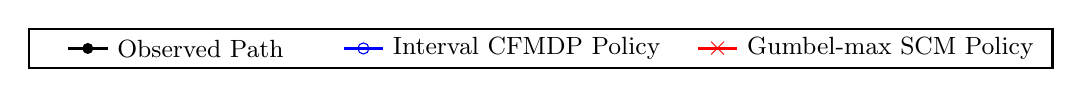
\begin{tikzpicture}[scale=1.0, every node/.style={scale=1.0}]
            \draw[thick, black] (-3, -0.25) rectangle (10, 0.25);
            %
            \draw[black, line width=1pt] (-2.5, 0.0) -- (-2,0.0);
            \fill[black] (-2.25,0.0) circle (2pt); %
            \node[right] at (-2,0.0) {\small Observed Path};
            
            %
            \draw[blue, line width=1pt] (1.0,0.0) -- (1.5,0.0);
            \node[draw=blue, circle, minimum size=4pt, inner sep=0pt] at (1.25,0.0) {}; %
            \node[right] at (1.5,0.0) {\small Interval CFMDP Policy};
            
            %
            \draw[red, line width=1pt] (5.5,0) -- (6,0);
            \node[red] at (5.75,0) {$\boldsymbol{\times}$}; %
            \node[right] at (6,0) {\small Gumbel-max SCM Policy};
        \end{tikzpicture}
    }\\
    %
    \subfigure[\footnotesize Lowest cumulative reward: Interval CFMDP ($312$), Gumbel-max SCM ($312$)]{%
        \resizebox{0.76\columnwidth}{!}{
             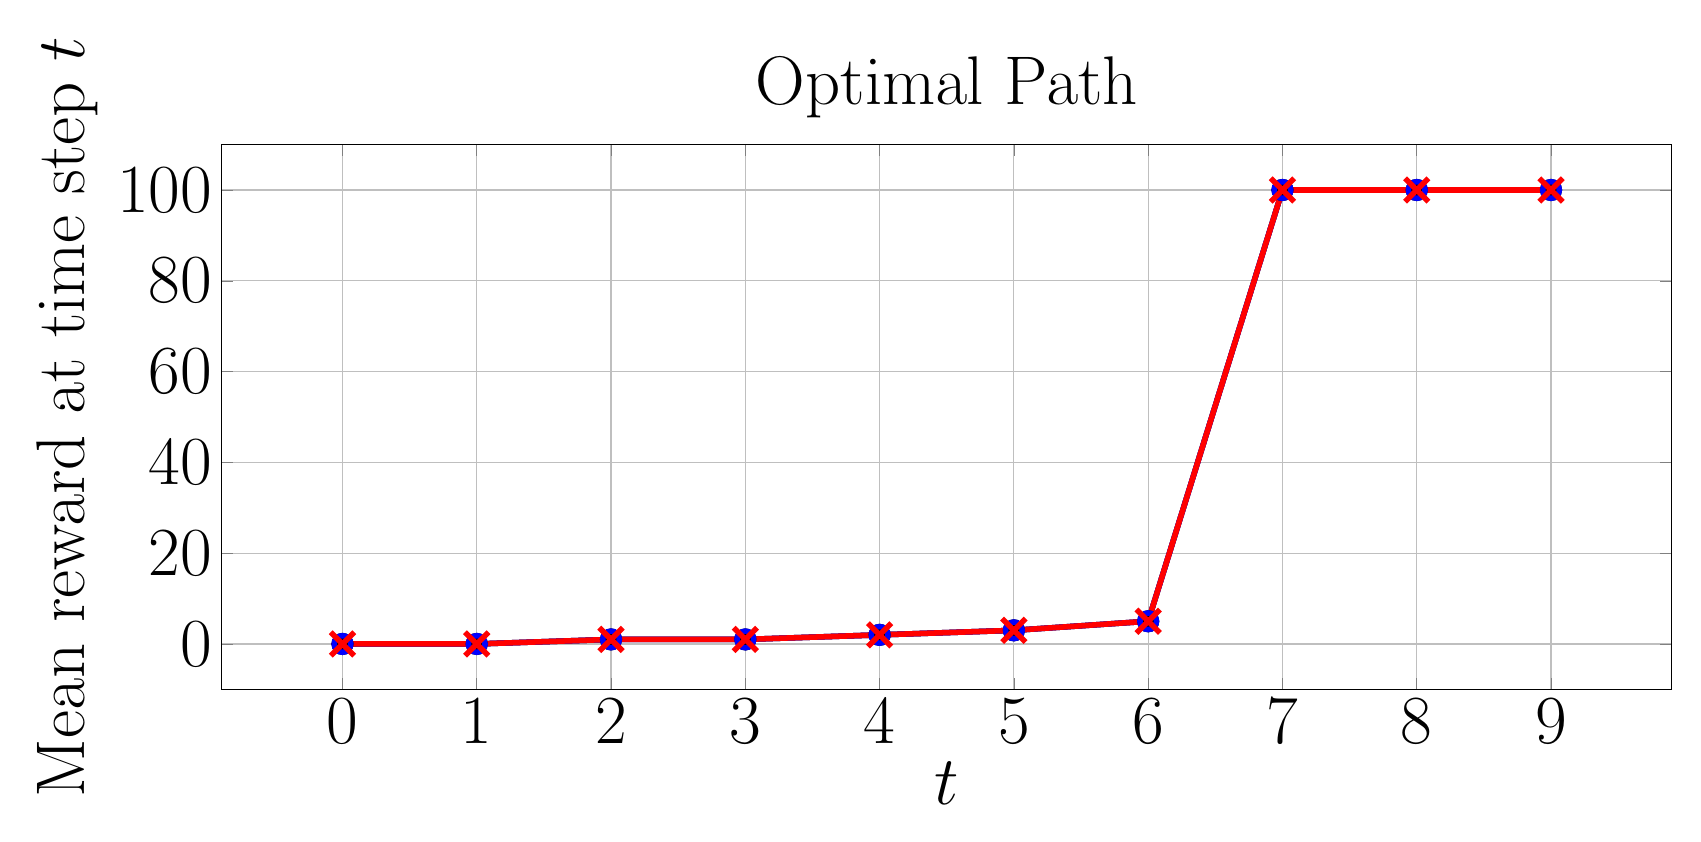
\begin{tikzpicture}
                \begin{axis}[
                    xlabel={$t$},
                    ylabel={Mean reward at time step $t$},
                    title={Optimal Path},
                    grid=both,
                    width=20cm, height=8.5cm,
                    every axis/.style={font=\Huge},
                    %
                ]
                \addplot[
                    color=black, %
                    mark=*, %
                    line width=2pt,
                    mark size=3pt,
                    error bars/.cd,
                    y dir=both, %
                    y explicit, %
                    error bar style={line width=1pt,solid},
                    error mark options={line width=1pt,mark size=4pt,rotate=90}
                ]
                coordinates {
                    (0, 0.0)  +- (0, 0.0)
                    (1, 0.0)  +- (0, 0.0) 
                    (2, 1.0)  +- (0, 0.0) 
                    (3, 1.0)  +- (0, 0.0)
                    (4, 2.0)  +- (0, 0.0)
                    (5, 3.0) +- (0, 0.0)
                    (6, 5.0) +- (0, 0.0)
                    (7, 100.0) +- (0, 0.0)
                    (8, 100.0) +- (0, 0.0)
                    (9, 100.0) +- (0, 0.0)
                };
                %
                \addplot[
                    color=blue, %
                    mark=o, %
                    line width=2pt,
                    mark size=3pt,
                    error bars/.cd,
                    y dir=both, %
                    y explicit, %
                    error bar style={line width=1pt,solid},
                    error mark options={line width=1pt,mark size=4pt,rotate=90}
                ]
                 coordinates {
                    (0, 0.0)  +- (0, 0.0)
                    (1, 0.0)  +- (0, 0.0) 
                    (2, 1.0)  +- (0, 0.0) 
                    (3, 1.0)  +- (0, 0.0)
                    (4, 2.0)  +- (0, 0.0)
                    (5, 3.0) +- (0, 0.0)
                    (6, 5.0) +- (0, 0.0)
                    (7, 100.0) +- (0, 0.0)
                    (8, 100.0) +- (0, 0.0)
                    (9, 100.0) +- (0, 0.0)
                };
                %
                \addplot[
                    color=red, %
                    mark=x, %
                    line width=2pt,
                    mark size=6pt,
                    error bars/.cd,
                    y dir=both, %
                    y explicit, %
                    error bar style={line width=1pt,solid},
                    error mark options={line width=1pt,mark size=4pt,rotate=90}
                ]
                coordinates {
                    (0, 0.0)  +- (0, 0.0)
                    (1, 0.0)  +- (0, 0.0) 
                    (2, 1.0)  +- (0, 0.0) 
                    (3, 1.0)  +- (0, 0.0)
                    (4, 2.0)  +- (0, 0.0)
                    (5, 3.0) +- (0, 0.0)
                    (6, 5.0) +- (0, 0.0)
                    (7, 100.0) +- (0, 0.0)
                    (8, 100.0) +- (0, 0.0)
                    (9, 100.0) +- (0, 0.0)
                };
                \end{axis}
            \end{tikzpicture}
         }
    }
    \hspace{1cm}
    \subfigure[\footnotesize Lowest cumulative reward: Interval CFMDP ($19$), Gumbel-max SCM ($-88$)]{%
         \resizebox{0.76\columnwidth}{!}{
            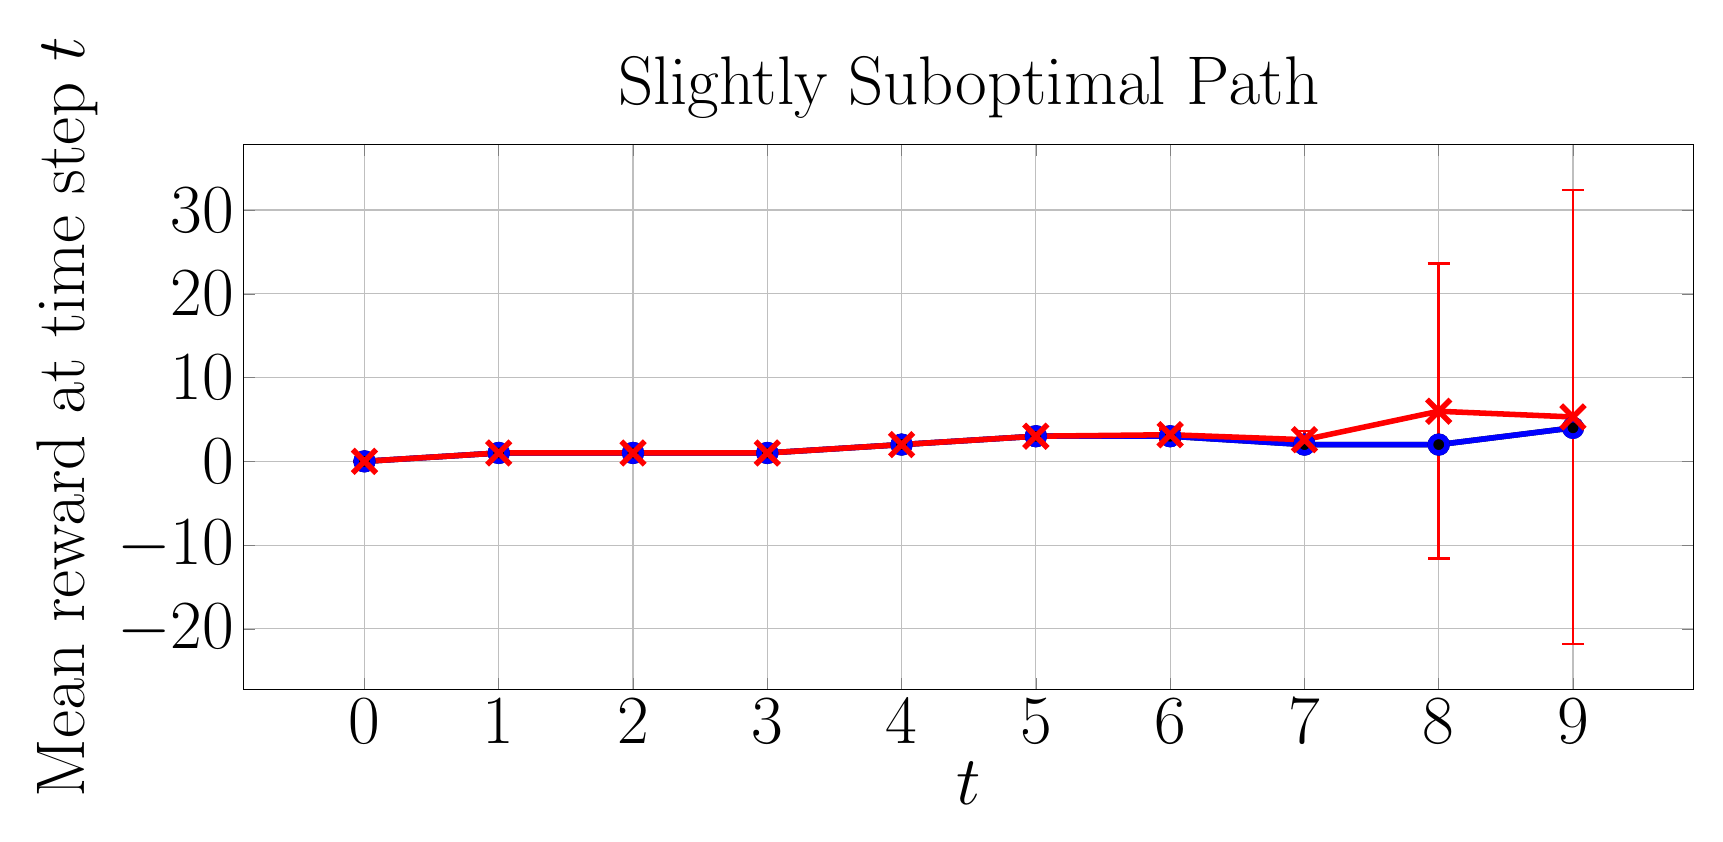
\begin{tikzpicture}
                \begin{axis}[
                    xlabel={$t$},
                    ylabel={Mean reward at time step $t$},
                    title={Slightly Suboptimal Path},
                    grid=both,
                    width=20cm, height=8.5cm,
                    every axis/.style={font=\Huge},
                    %
                ]
                \addplot[
                    color=black, %
                    mark=*, %
                    line width=2pt,
                    mark size=3pt,
                    error bars/.cd,
                    y dir=both, %
                    y explicit, %
                    error bar style={line width=1pt,solid},
                    error mark options={line width=1pt,mark size=4pt,rotate=90}
                ]
              coordinates {
                    (0, 0.0)  +- (0, 0.0)
                    (1, 1.0)  +- (0, 0.0) 
                    (2, 1.0)  +- (0, 0.0) 
                    (3, 1.0)  +- (0, 0.0)
                    (4, 2.0)  +- (0, 0.0)
                    (5, 3.0) +- (0, 0.0)
                    (6, 3.0) +- (0, 0.0)
                    (7, 2.0) +- (0, 0.0)
                    (8, 2.0) +- (0, 0.0)
                    (9, 4.0) +- (0, 0.0)
                };
                %
                \addplot[
                    color=blue, %
                    mark=o, %
                    line width=2pt,
                    mark size=3pt,
                    error bars/.cd,
                    y dir=both, %
                    y explicit, %
                    error bar style={line width=1pt,solid},
                    error mark options={line width=1pt,mark size=4pt,rotate=90}
                ]
              coordinates {
                    (0, 0.0)  +- (0, 0.0)
                    (1, 1.0)  +- (0, 0.0) 
                    (2, 1.0)  +- (0, 0.0) 
                    (3, 1.0)  +- (0, 0.0)
                    (4, 2.0)  +- (0, 0.0)
                    (5, 3.0) +- (0, 0.0)
                    (6, 3.0) +- (0, 0.0)
                    (7, 2.0) +- (0, 0.0)
                    (8, 2.0) +- (0, 0.0)
                    (9, 4.0) +- (0, 0.0)
                };
                %
                \addplot[
                    color=red, %
                    mark=x, %
                    line width=2pt,
                    mark size=6pt,
                    error bars/.cd,
                    y dir=both, %
                    y explicit, %
                    error bar style={line width=1pt,solid},
                    error mark options={line width=1pt,mark size=4pt,rotate=90}
                ]
                coordinates {
                    (0, 0.0)  +- (0, 0.0)
                    (1, 1.0)  +- (0, 0.0) 
                    (2, 1.0)  +- (0, 0.0) 
                    (3, 1.0)  +- (0, 0.0)
                    (4, 2.0)  += (0, 0.0)
                    (5, 3.0)  += (0, 0.0)
                    (6, 3.17847) += (0, 0.62606746) -= (0, 0.62606746)
                    (7, 2.5832885) += (0, 1.04598233) -= (0, 1.04598233)
                    (8, 5.978909) += (0, 17.60137623) -= (0, 17.60137623)
                    (9, 5.297059) += (0, 27.09227512) -= (0, 27.09227512)
                };
                \end{axis}
            \end{tikzpicture}
         }
    }\\[-1.5pt]
    \subfigure[\footnotesize Lowest cumulative reward: Interval CFMDP ($14$), Gumbel-max SCM ($-598$)]{%
         \resizebox{0.76\columnwidth}{!}{
             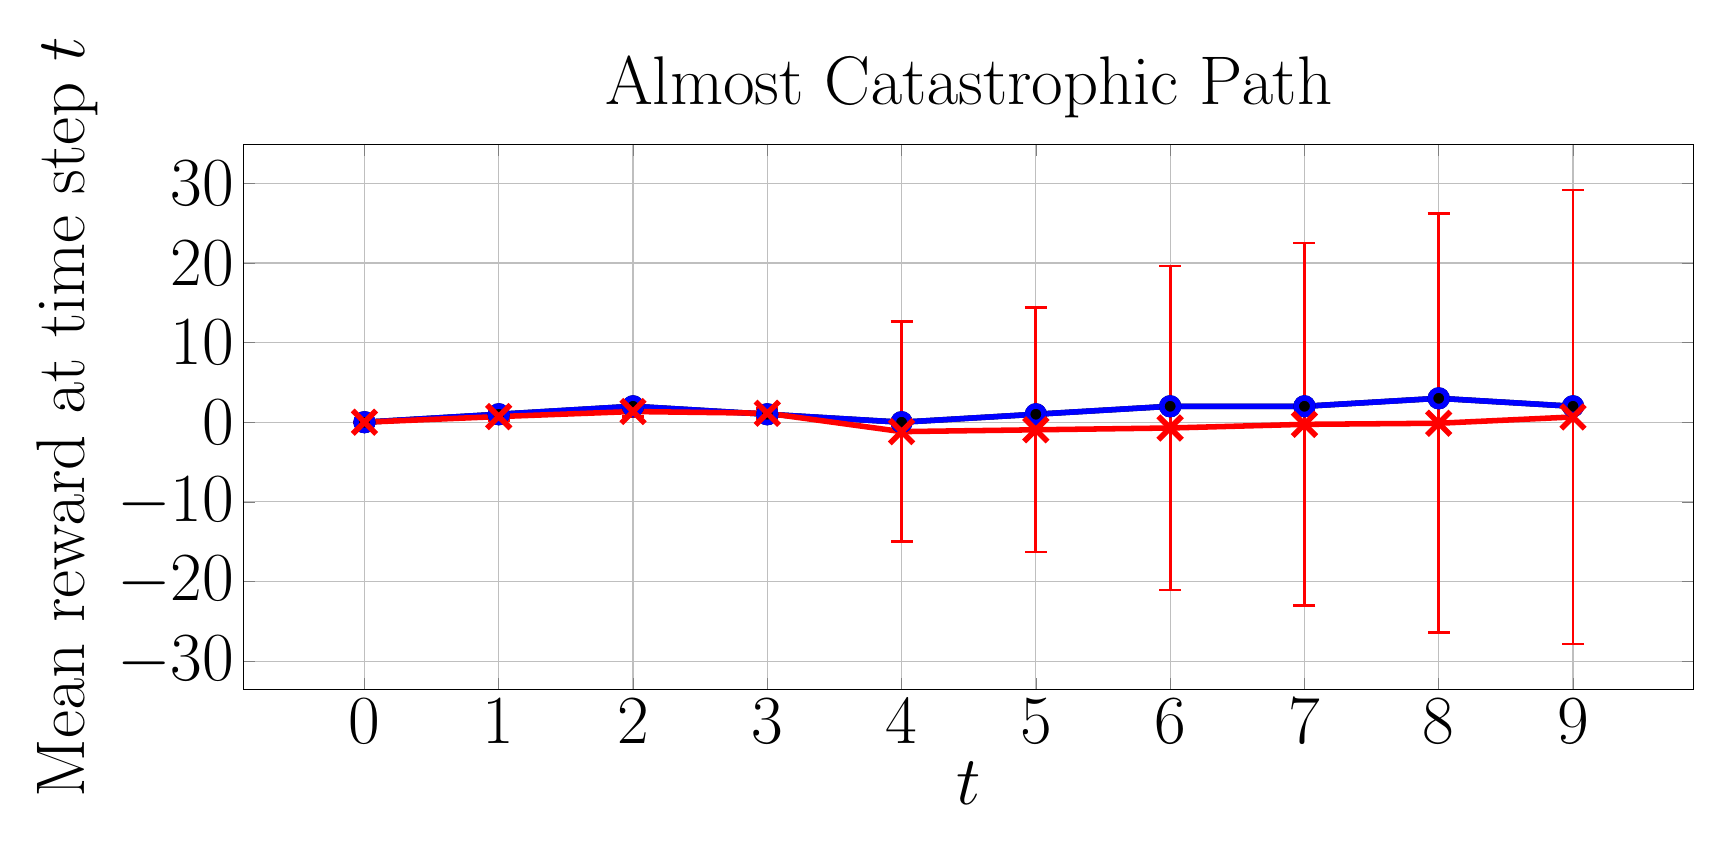
\begin{tikzpicture}
                \begin{axis}[
                    xlabel={$t$},
                    ylabel={Mean reward at time step $t$},
                    title={Almost Catastrophic Path},
                    grid=both,
                    width=20cm, height=8.5cm,
                    every axis/.style={font=\Huge},
                    %
                ]
                \addplot[
                    color=black, %
                    mark=*, %
                    line width=2pt,
                    mark size=3pt,
                    error bars/.cd,
                    y dir=both, %
                    y explicit, %
                    error bar style={line width=1pt,solid},
                    error mark options={line width=1pt,mark size=4pt,rotate=90}
                ]
                coordinates {
                    (0, 0.0)  +- (0, 0.0)
                    (1, 1.0)  +- (0, 0.0) 
                    (2, 2.0)  +- (0, 0.0) 
                    (3, 1.0)  +- (0, 0.0)
                    (4, 0.0)  +- (0, 0.0)
                    (5, 1.0) +- (0, 0.0)
                    (6, 2.0) +- (0, 0.0)
                    (7, 2.0) +- (0, 0.0)
                    (8, 3.0) +- (0, 0.0)
                    (9, 2.0) +- (0, 0.0)
                };
                %
                \addplot[
                    color=blue, %
                    mark=o, %
                    line width=2pt,
                    mark size=3pt,
                    error bars/.cd,
                    y dir=both, %
                    y explicit, %
                    error bar style={line width=1pt,solid},
                    error mark options={line width=1pt,mark size=4pt,rotate=90}
                ]
                coordinates {
                    (0, 0.0)  +- (0, 0.0)
                    (1, 1.0)  +- (0, 0.0) 
                    (2, 2.0)  +- (0, 0.0) 
                    (3, 1.0)  +- (0, 0.0)
                    (4, 0.0)  +- (0, 0.0)
                    (5, 1.0) +- (0, 0.0)
                    (6, 2.0) +- (0, 0.0)
                    (7, 2.0) +- (0, 0.0)
                    (8, 3.0) +- (0, 0.0)
                    (9, 2.0) +- (0, 0.0)
                };
                %
                \addplot[
                    color=red, %
                    mark=x, %
                    line width=2pt,
                    mark size=6pt,
                    error bars/.cd,
                    y dir=both, %
                    y explicit, %
                    error bar style={line width=1pt,solid},
                    error mark options={line width=1pt,mark size=4pt,rotate=90}
                ]
                coordinates {
                    (0, 0.0)  +- (0, 0.0)
                    (1, 0.7065655)  +- (0, 0.4553358) 
                    (2, 1.341673)  +- (0, 0.67091621) 
                    (3, 1.122926)  +- (0, 0.61281824)
                    (4, -1.1821935)  +- (0, 13.82444042)
                    (5, -0.952399)  +- (0, 15.35195457)
                    (6, -0.72672) +- (0, 20.33508414)
                    (7, -0.268983) +- (0, 22.77861454)
                    (8, -0.1310835) +- (0, 26.31013314)
                    (9, 0.65806) +- (0, 28.50670214)
                };
                %
            %
            %
            %
            %
            %
            %
            %
            %
            %
            %
            %
            %
            %
            %
            %
            %
            %
            %
                \end{axis}
            \end{tikzpicture}
         }
    }
    \hspace{1cm}
    \subfigure[\footnotesize Lowest cumulative reward: Interval CFMDP ($-698$), Gumbel-max SCM ($-698$)]{%
         \resizebox{0.76\columnwidth}{!}{
            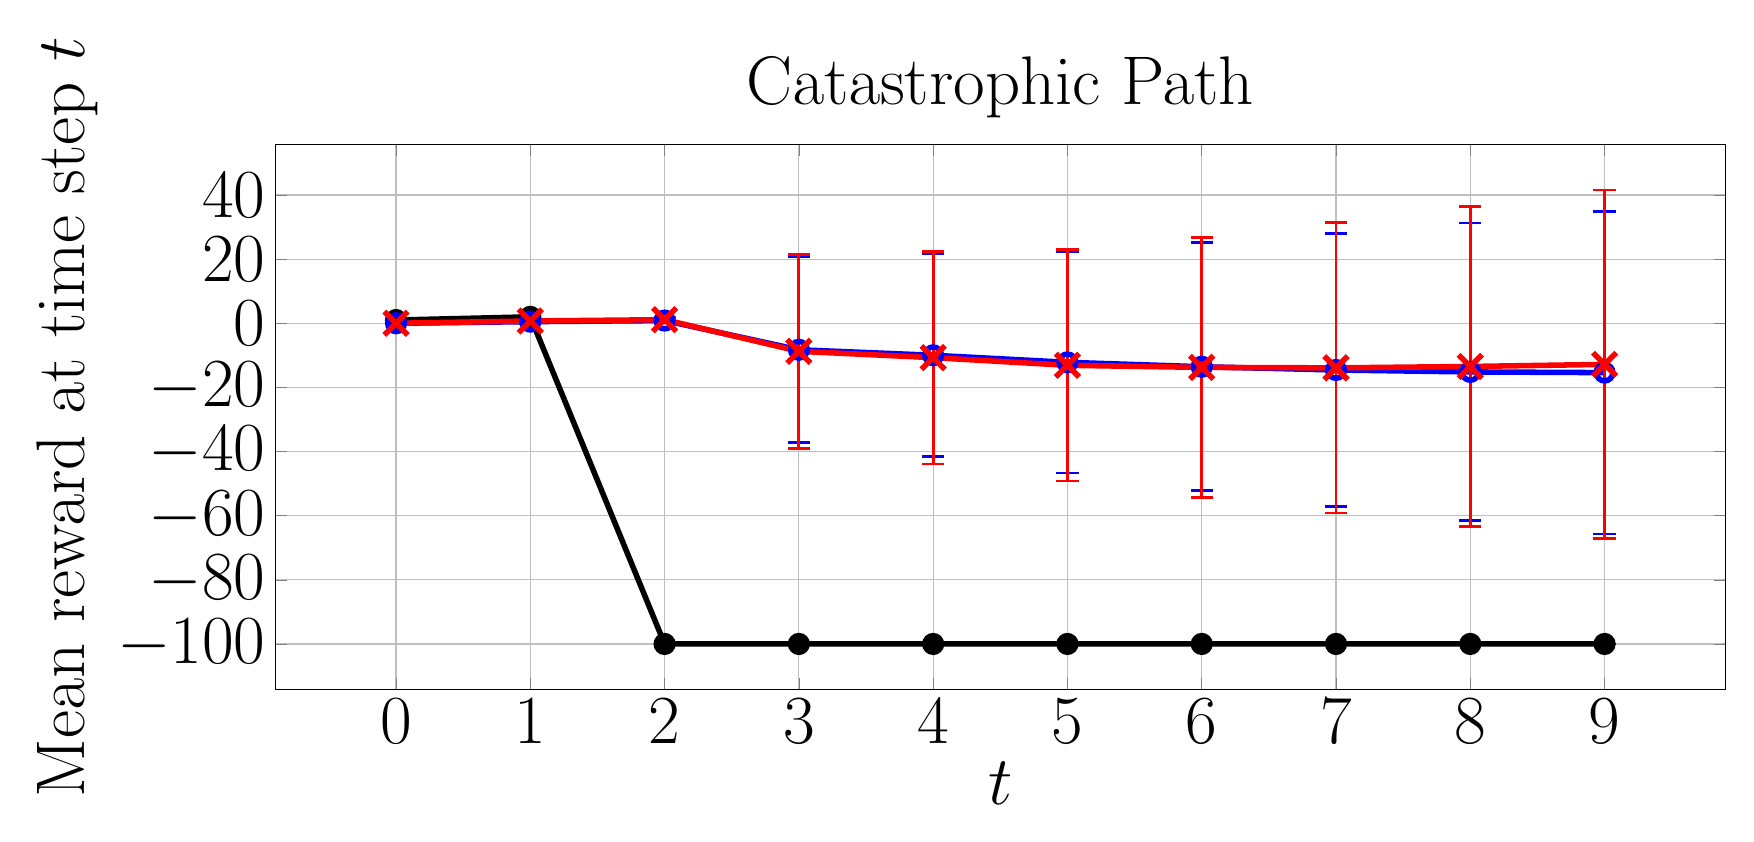
\begin{tikzpicture}
                \begin{axis}[
                    xlabel={$t$},
                    ylabel={Mean reward at time step $t$},
                    title={Catastrophic Path},
                    grid=both,
                    width=20cm, height=8.5cm,
                    every axis/.style={font=\Huge},
                    %
                ]
                \addplot[
                    color=black, %
                    mark=*, %
                    line width=2pt,
                    mark size=3pt,
                    error bars/.cd,
                    y dir=both, %
                    y explicit, %
                    error bar style={line width=1pt,solid},
                    error mark options={line width=1pt,mark size=4pt,rotate=90}
                ]
                coordinates {
                    (0, 1.0)  +- (0, 0.0)
                    (1, 2.0)  +- (0, 0.0) 
                    (2, -100.0)  +- (0, 0.0) 
                    (3, -100.0)  +- (0, 0.0)
                    (4, -100.0)  +- (0, 0.0)
                    (5, -100.0) +- (0, 0.0)
                    (6, -100.0) +- (0, 0.0)
                    (7, -100.0) +- (0, 0.0)
                    (8, -100.0) +- (0, 0.0)
                    (9, -100.0) +- (0, 0.0)
                };
                %
                \addplot[
                    color=blue, %
                    mark=o, %
                    line width=2pt,
                    mark size=3pt,
                    error bars/.cd,
                    y dir=both, %
                    y explicit, %
                    error bar style={line width=1pt,solid},
                    error mark options={line width=1pt,mark size=4pt,rotate=90}
                ]
                coordinates {
                    (0, 0.0)  +- (0, 0.0)
                    (1, 0.504814)  +- (0, 0.49997682) 
                    (2, 0.8439835)  +- (0, 0.76831917) 
                    (3, -8.2709165)  +- (0, 28.93656754)
                    (4, -9.981082)  +- (0, 31.66825363)
                    (5, -12.1776325) +- (0, 34.53463233)
                    (6, -13.556076) +- (0, 38.62845372)
                    (7, -14.574418) +- (0, 42.49603359)
                    (8, -15.1757075) +- (0, 46.41913968)
                    (9, -15.3900395) +- (0, 50.33563368)
                };
                %
                \addplot[
                    color=red, %
                    mark=x, %
                    line width=2pt,
                    mark size=6pt,
                    error bars/.cd,
                    y dir=both, %
                    y explicit, %
                    error bar style={line width=1pt,solid},
                    error mark options={line width=1pt,mark size=4pt,rotate=90}
                ]
                coordinates {
                    (0, 0.0)  +- (0, 0.0)
                    (1, 0.701873)  +- (0, 0.45743556) 
                    (2, 1.1227805)  +- (0, 0.73433129) 
                    (3, -8.7503255)  +- (0, 30.30257976)
                    (4, -10.722092)  +- (0, 33.17618589)
                    (5, -13.10721)  +- (0, 36.0648089)
                    (6, -13.7631645) +- (0, 40.56553451)
                    (7, -13.909043) +- (0, 45.23829402)
                    (8, -13.472517) +- (0, 49.96270296)
                    (9, -12.8278835) +- (0, 54.38618735)
                };
                %
            %
            %
            %
            %
            %
            %
            %
            %
            %
            %
            %
            %
            %
            %
            %
            %
            %
            %
                \end{axis}
            \end{tikzpicture}
         }
    }
    \caption{Average instant reward of CF paths induced by policies on GridWorld $p=0.4$.}
    \label{fig: reward p=0.4}
\end{figure*}

\subsection{Experimental Setup}
To compare policy performance, we measure the average rewards of counterfactual paths induced by our policy and the Gumbel-max policy by uniformly sampling $200$ counterfactual MDPs from the ICFMDP and generating $10,000$ counterfactual paths over each sampled CFMDP. \jl{Since the interval CFMDP depends on the observed path, we select $4$  paths of varying optimality to evaluate how the observed path impacts the performance of both policies: an optimal path, a slightly suboptimal path that could reach the optimal reward with a few changes, a catastrophic path that enters a catastrophic, terminal state with low reward, and an almost catastrophic path that was close to entering a catastrophic state.} When measuring the average probability bound widths and execution time needed to generate the ICFMDPs, we averaged over $20$ randomly generated observed paths
\footnote{Further training details are provided in Appendix \ref{app: training details}, and the code is provided at \href{https://github.com/ddv-lab/robust-cf-inference-in-MDPs}{https://github.com/ddv-lab/robust-cf-inference-in-MDPs}
%
%
.}.

\subsection{GridWorld}
\jl{The GridWorld MDP is a $4 \times 4$ grid where an agent must navigate from the top-left corner to the goal state in the bottom-right corner, avoiding a dangerous terminal state in the centre. At each time step, the agent can move up, down, left, or right, but there is a small probability (controlled by hyper-parameter $p$) of moving in an unintended direction. As the agent nears the goal, the reward for each state increases, culminating in a reward of $+100$ for reaching the goal. Entering the dangerous state results in a penalty of $-100$. We use two versions of GridWorld: a less stochastic version with $p=0.9$ (i.e., $90$\% chance of moving in the chosen direction) and a more stochastic version with $p=0.4$.}

\paragraph{GridWorld ($p=0.9$)}
When $p=0.9$, the counterfactual probability bounds are typically narrow (see Table \ref{tab:nonzero_probs} for average measurements). Consequently, as shown in Figure \ref{fig: reward p=0.9}, both policies are nearly identical and perform similarly well across the optimal, slightly suboptimal, and catastrophic paths.
%
However, for the almost catastrophic path, the interval CFMDP path is more conservative and follows the observed path more closely (as this is where the probability bounds are narrowest), which typically requires one additional step to reach the goal state than the Gumbel-max SCM policy.
%

\paragraph{GridWorld ($p=0.4$)}
\jl{When $p=0.4$, the GridWorld environment becomes more uncertain, increasing the risk of entering the dangerous state even if correct actions are chosen. Thus, as shown in Figure \ref{fig: reward p=0.4}, the interval CFMDP policy adopts a more conservative approach, avoiding deviation from the observed policy if it cannot guarantee higher counterfactual rewards (see the slightly suboptimal and almost catastrophic paths), whereas the Gumbel-max SCM is inconsistent: it can yield higher rewards, but also much lower rewards, reflected in the wide error bars.} For the catastrophic path, both policies must deviate from the observed path to achieve a higher reward and, in this case, perform similarly.
%
%
%
%
\subsection{Sepsis}
The Sepsis MDP \citep{oberst2019counterfactual} simulates trajectories of Sepsis patients. Each state consists of four vital signs (heart rate, blood pressure, oxygen concentration, and glucose levels), categorised as low, normal, or high.
and three treatments that can be toggled on/off at each time step (8 actions in total). Unlike \citet{oberst2019counterfactual}, we scale rewards based on the number of out-of-range vital signs, between $-1000$ (patient dies) and $1000$ (patient discharged). \jl{Like the GridWorld $p=0.4$ experiment, the Sepsis MDP is highly uncertain, as many states are equally likely to lead to optimal and poor outcomes. Thus, as shown in Figure \ref{fig: reward sepsis}, both policies follow the observed optimal and almost catastrophic paths to guarantee rewards are no worse than the observation.} However, improving the catastrophic path requires deviating from the observation. Here, the Gumbel-max SCM policy, on average, performs better than the interval CFMDP policy. But, since both policies have lower bounds clipped at $-1000$, neither policy reliably improves over the observation. In contrast, for the slightly suboptimal path, the interval CFMDP policy performs significantly better, shown by its higher lower bounds. 
Moreover, in these two cases, the worst-case counterfactual path generated by the interval CFMDP policy is better than that of the Gumbel-max SCM policy,
indicating its greater robustness.
%
\begin{figure*}
    \centering
     \resizebox{0.6\textwidth}{!}{
        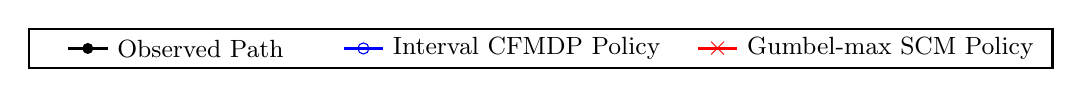
\begin{tikzpicture}[scale=1.0, every node/.style={scale=1.0}]
            \draw[thick, black] (-3, -0.25) rectangle (10, 0.25);
            %
            \draw[black, line width=1pt] (-2.5, 0.0) -- (-2,0.0);
            \fill[black] (-2.25,0.0) circle (2pt); %
            \node[right] at (-2,0.0) {\small Observed Path};
            
            %
            \draw[blue, line width=1pt] (1.0,0.0) -- (1.5,0.0);
            \node[draw=blue, circle, minimum size=4pt, inner sep=0pt] at (1.25,0.0) {}; %
            \node[right] at (1.5,0.0) {\small Interval CFMDP Policy};
            
            %
            \draw[red, line width=1pt] (5.5,0) -- (6,0);
            \node[red] at (5.75,0) {$\boldsymbol{\times}$}; %
            \node[right] at (6,0) {\small Gumbel-max SCM Policy};
        \end{tikzpicture}
    }\\
    \subfigure[\footnotesize Lowest cumulative reward: Interval CFMDP ($8000$), Gumbel-max SCM ($8000$)]{%
         \resizebox{0.76\columnwidth}{!}{
             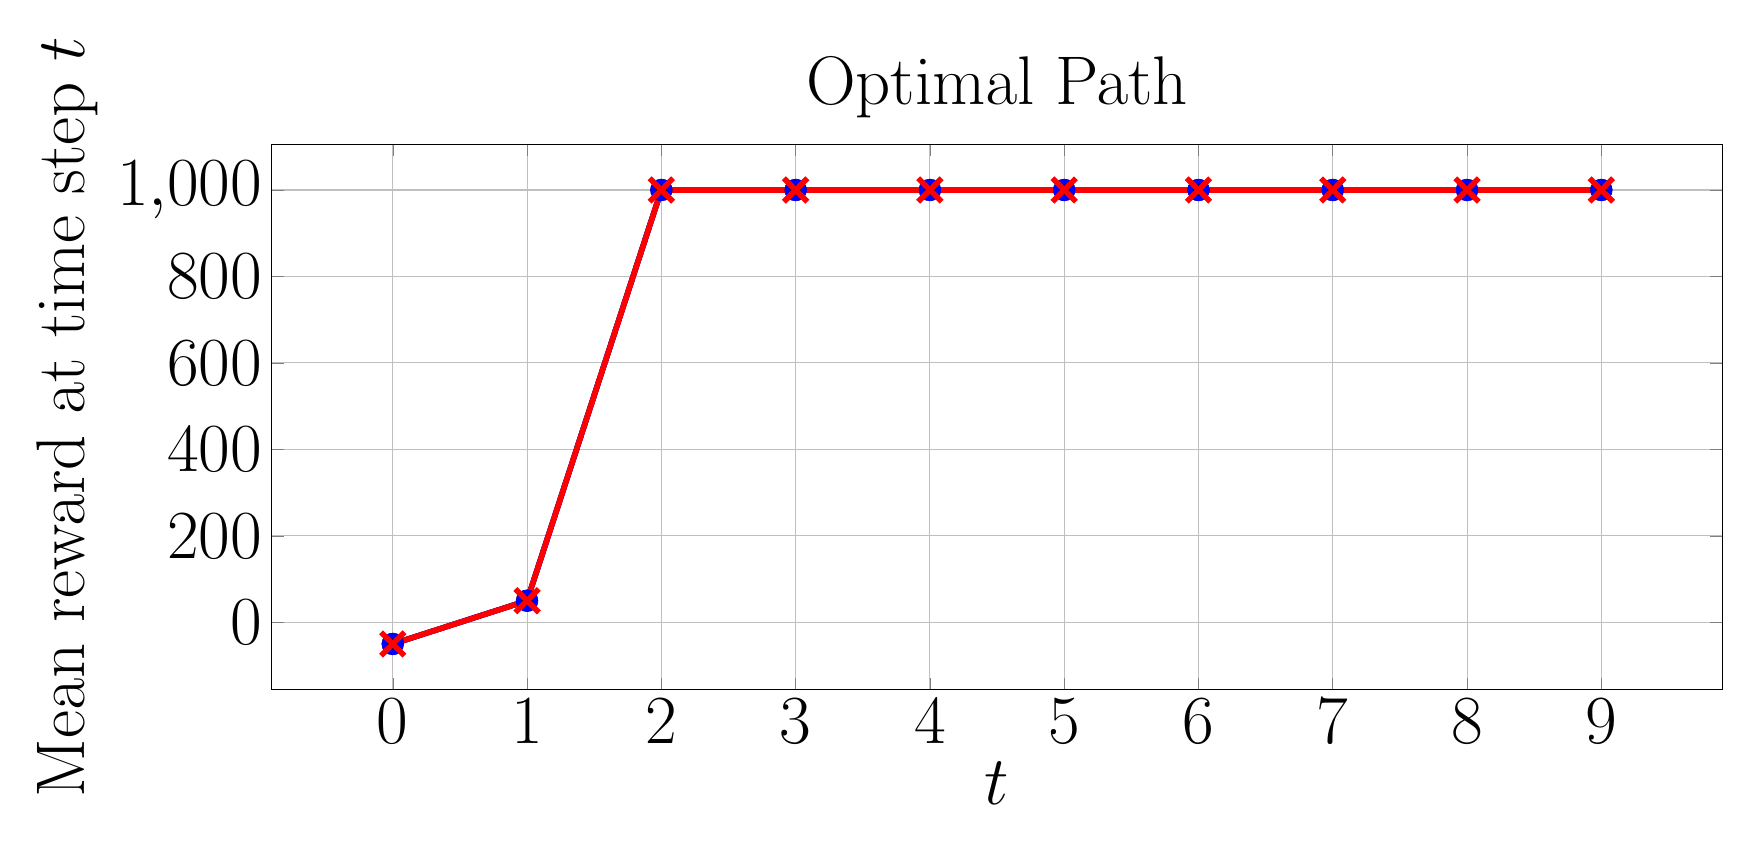
\begin{tikzpicture}
                \begin{axis}[
                    xlabel={$t$},
                    ylabel={Mean reward at time step $t$},
                    title={Optimal Path},
                    grid=both,
                    width=20cm, height=8.5cm,
                    every axis/.style={font=\Huge},
                    %
                ]
                \addplot[
                    color=black, %
                    mark=*, %
                    line width=2pt,
                    mark size=3pt,
                ]
                coordinates {
                    (0, -50.0)
                    (1, 50.0)
                    (2, 1000.0)
                    (3, 1000.0)
                    (4, 1000.0)
                    (5, 1000.0)
                    (6, 1000.0)
                    (7, 1000.0)
                    (8, 1000.0)
                    (9, 1000.0)
                };
                %
                \addplot[
                    color=blue, %
                    mark=o, %
                    line width=2pt,
                    mark size=3pt,
                    error bars/.cd,
                    y dir=both, %
                    y explicit, %
                    error bar style={line width=1pt,solid},
                    error mark options={line width=1pt,mark size=4pt,rotate=90}
                ]
                coordinates {
                    (0, -50.0)  +- (0, 0.0)
                    (1, 50.0)  +- (0, 0.0) 
                    (2, 1000.0)  +- (0, 0.0) 
                    (3, 1000.0)  +- (0, 0.0)
                    (4, 1000.0)  +- (0, 0.0)
                    (5, 1000.0) +- (0, 0.0)
                    (6, 1000.0) +- (0, 0.0)
                    (7, 1000.0) +- (0, 0.0)
                    (8, 1000.0) +- (0, 0.0)
                    (9, 1000.0) +- (0, 0.0)
                };
                %
                \addplot[
                    color=red, %
                    mark=x, %
                    line width=2pt,
                    mark size=6pt,
                    error bars/.cd,
                    y dir=both, %
                    y explicit, %
                    error bar style={line width=1pt,solid},
                    error mark options={line width=1pt,mark size=4pt,rotate=90}
                ]
                coordinates {
                    (0, -50.0)  +- (0, 0.0)
                    (1, 50.0)  +- (0, 0.0) 
                    (2, 1000.0)  +- (0, 0.0) 
                    (3, 1000.0)  +- (0, 0.0)
                    (4, 1000.0)  +- (0, 0.0)
                    (5, 1000.0) +- (0, 0.0)
                    (6, 1000.0) +- (0, 0.0)
                    (7, 1000.0) +- (0, 0.0)
                    (8, 1000.0) +- (0, 0.0)
                    (9, 1000.0) +- (0, 0.0)
                };
                %
                \end{axis}
            \end{tikzpicture}
         }
    }
    \hspace{1cm}
    \subfigure[\footnotesize Lowest cumulative reward: Interval CFMDP ($-5980$), Gumbel-max SCM ($-8000$)]{%
         \resizebox{0.76\columnwidth}{!}{
            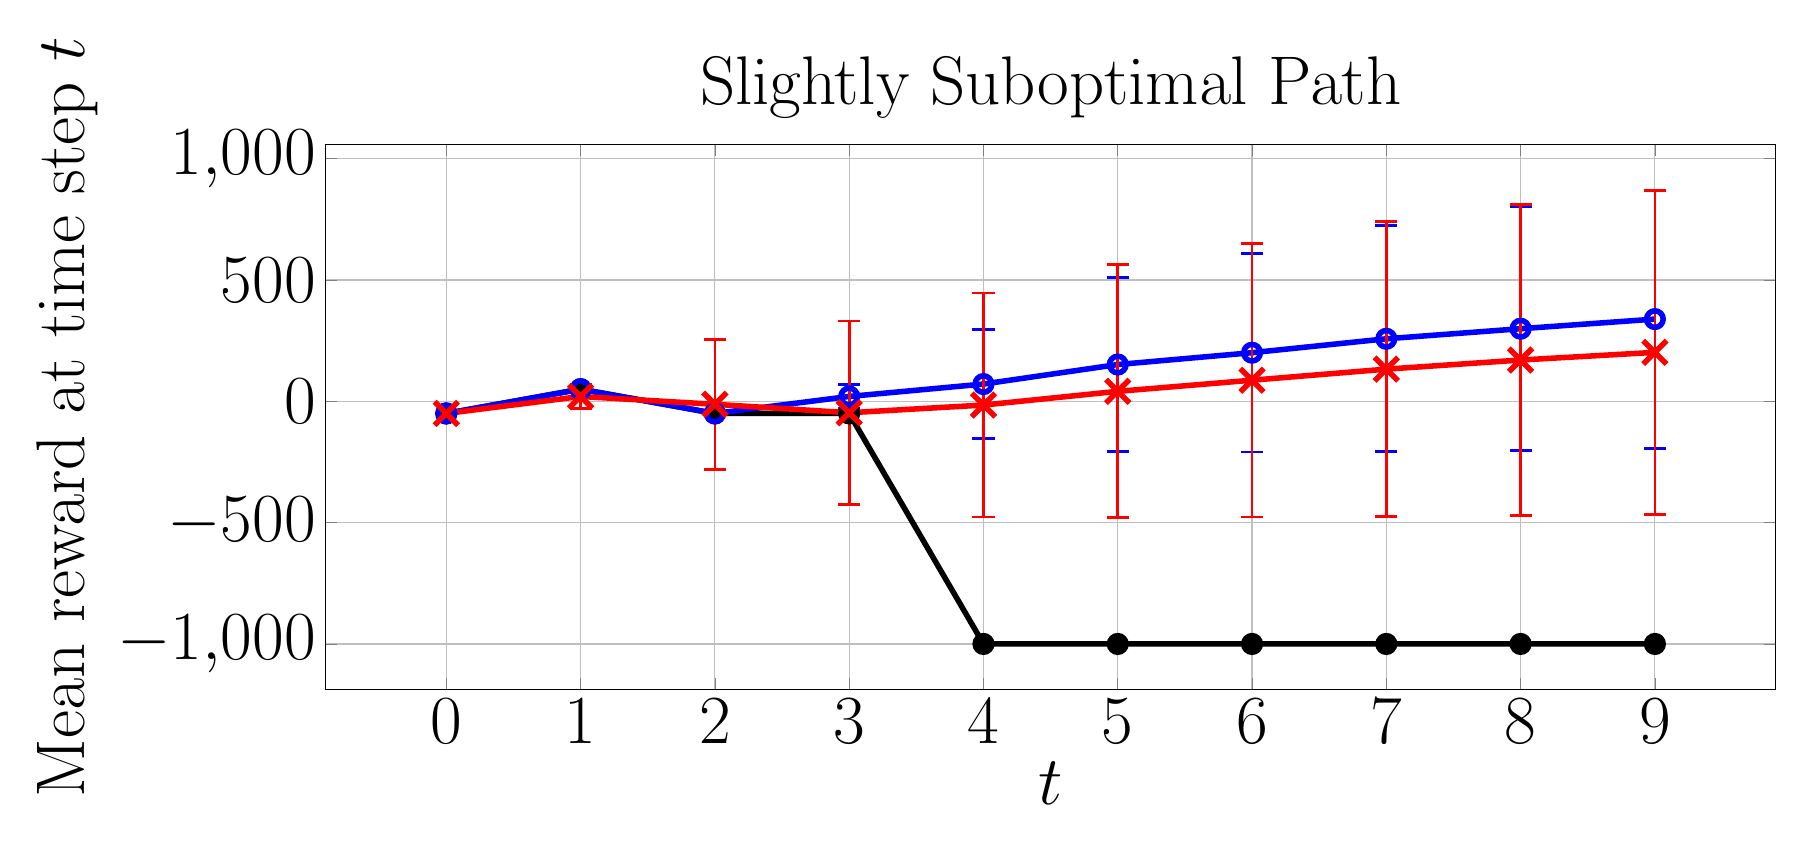
\begin{tikzpicture}
                \begin{axis}[
                    xlabel={$t$},
                    ylabel={Mean reward at time step $t$},
                    title={Slightly Suboptimal Path},
                    grid=both,
                    width=20cm, height=8.5cm,
                    every axis/.style={font=\Huge},
                    %
                ]
               \addplot[
                    color=black, %
                    mark=*, %
                    line width=2pt,
                    mark size=3pt,
                ]
                coordinates {
                    (0, -50.0)
                    (1, 50.0)
                    (2, -50.0)
                    (3, -50.0)
                    (4, -1000.0)
                    (5, -1000.0)
                    (6, -1000.0)
                    (7, -1000.0)
                    (8, -1000.0)
                    (9, -1000.0)
                };
                %
                \addplot[
                    color=blue, %
                    mark=o, %
                    line width=2pt,
                    mark size=3pt,
                    error bars/.cd,
                    y dir=both, %
                    y explicit, %
                    error bar style={line width=1pt,solid},
                    error mark options={line width=1pt,mark size=4pt,rotate=90}
                ]
                coordinates {
                    (0, -50.0)  +- (0, 0.0)
                    (1, 50.0)  +- (0, 0.0) 
                    (2, -50.0)  +- (0, 0.0) 
                    (3, 20.0631)  +- (0, 49.97539413)
                    (4, 71.206585)  +- (0, 226.02033693)
                    (5, 151.60797) +- (0, 359.23292559)
                    (6, 200.40593) +- (0, 408.86185176)
                    (7, 257.77948) +- (0, 466.10372804)
                    (8, 299.237465) +- (0, 501.82579506)
                    (9, 338.9129) +- (0, 532.06124996)
                };
                %
                \addplot[
                    color=red, %
                    mark=x, %
                    line width=2pt,
                    mark size=6pt,
                    error bars/.cd,
                    y dir=both, %
                    y explicit, %
                    error bar style={line width=1pt,solid},
                    error mark options={line width=1pt,mark size=4pt,rotate=90}
                ]
                coordinates {
                    (0, -50.0)  +- (0, 0.0)
                    (1, 20.00736)  +- (0, 49.99786741) 
                    (2, -12.282865)  +- (0, 267.598755) 
                    (3, -47.125995)  +- (0, 378.41755832)
                    (4, -15.381965)  +- (0, 461.77616558)
                    (5, 41.15459) +- (0, 521.53189262)
                    (6, 87.01595) +- (0, 564.22243126 )
                    (7, 132.62376) +- (0, 607.31338037)
                    (8, 170.168145) +- (0, 641.48013693)
                    (9, 201.813135) +- (0, 667.29441777)
                };
                %
                %
                %
                %
                %
                %
                %
                %
                %
                %
                %
                %
                %
                %
                %
                %
                %
                %
                %
                \end{axis}
            \end{tikzpicture}
         }
    }\\[-1.5pt]
    \subfigure[\footnotesize Lowest cumulative reward: Interval CFMDP ($100$), Gumbel-max SCM ($100$)]{%
         \resizebox{0.76\columnwidth}{!}{
             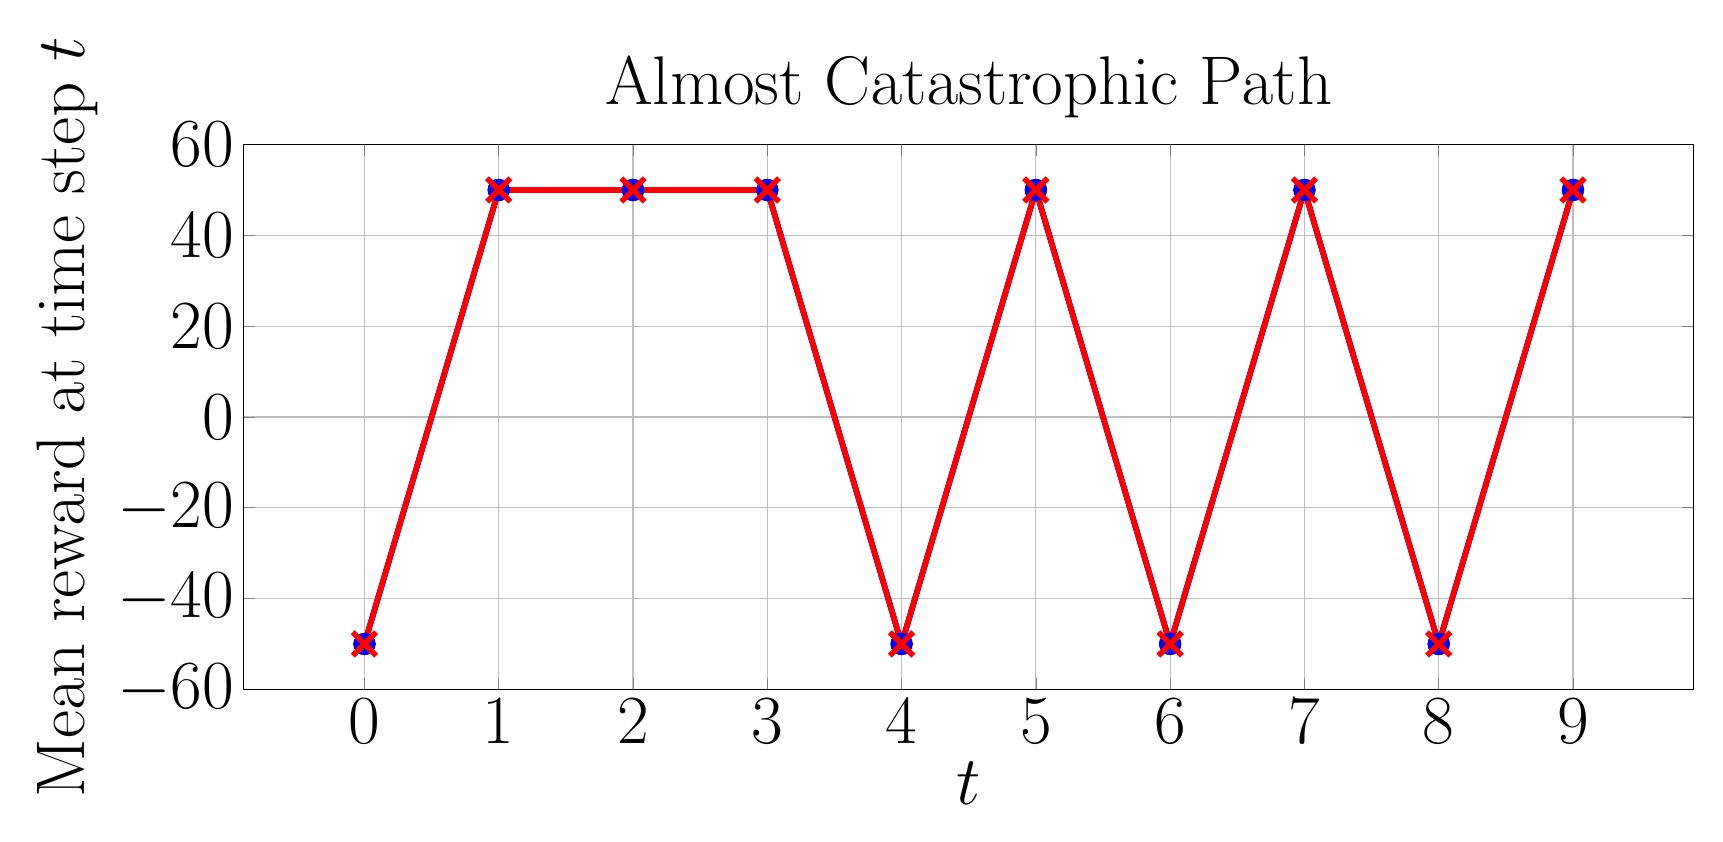
\begin{tikzpicture}
                \begin{axis}[
                    xlabel={$t$},
                    ylabel={Mean reward at time step $t$},
                    title={Almost Catastrophic Path},
                    grid=both,
                    every axis/.style={font=\Huge},
                    width=20cm, height=8.5cm,
                    %
                ]
               \addplot[
                    color=black, %
                    mark=*, %
                    line width=2pt,
                    mark size=3pt,
                ]
                coordinates {
                    (0, -50.0)
                    (1, 50.0)
                    (2, 50.0)
                    (3, 50.0)
                    (4, -50.0)
                    (5, 50.0)
                    (6, -50.0)
                    (7, 50.0)
                    (8, -50.0)
                    (9, 50.0)
                };
                %
                %
                \addplot[
                    color=blue, %
                    mark=o, %
                    line width=2pt,
                    mark size=3pt,
                    error bars/.cd,
                    y dir=both, %
                    y explicit, %
                    error bar style={line width=1pt,solid},
                    error mark options={line width=1pt,mark size=4pt,rotate=90}
                ]
                coordinates {
                    (0, -50.0)  +- (0, 0.0)
                    (1, 50.0)  +- (0, 0.0) 
                    (2, 50.0)  +- (0, 0.0) 
                    (3, 50.0)  +- (0, 0.0)
                    (4, -50.0)  +- (0, 0.0)
                    (5, 50.0) +- (0, 0.0)
                    (6, -50.0) +- (0, 0.0)
                    (7, 50.0) +- (0, 0.0)
                    (8, -50.0) +- (0, 0.0)
                    (9, 50.0) +- (0, 0.0)
                };
                %
                \addplot[
                    color=red, %
                    mark=x, %
                    line width=2pt,
                    mark size=6pt,
                    error bars/.cd,
                    y dir=both, %
                    y explicit, %
                    error bar style={line width=1pt,solid},
                    error mark options={line width=1pt,mark size=4pt,rotate=90}
                ]
                coordinates {
                    (0, -50.0)  +- (0, 0.0)
                    (1, 50.0)  +- (0, 0.0) 
                    (2, 50.0)  +- (0, 0.0) 
                    (3, 50.0)  +- (0, 0.0)
                    (4, -50.0)  +- (0, 0.0)
                    (5, 50.0) +- (0, 0.0)
                    (6, -50.0) +- (0, 0.0)
                    (7, 50.0) +- (0, 0.0)
                    (8, -50.0) +- (0, 0.0)
                    (9, 50.0) +- (0, 0.0)
                };
                %
                %
                %
                %
                %
                %
                %
                %
                %
                %
                %
                %
                %
                %
                %
                %
                %
                %
                %
                \end{axis}
            \end{tikzpicture}
         }
    }
    \hspace{1cm}
    \subfigure[\footnotesize Lowest cumulative reward: Interval CFMDP ($-7150$), Gumbel-max SCM ($-9050$)]{%
         \resizebox{0.76\columnwidth}{!}{
            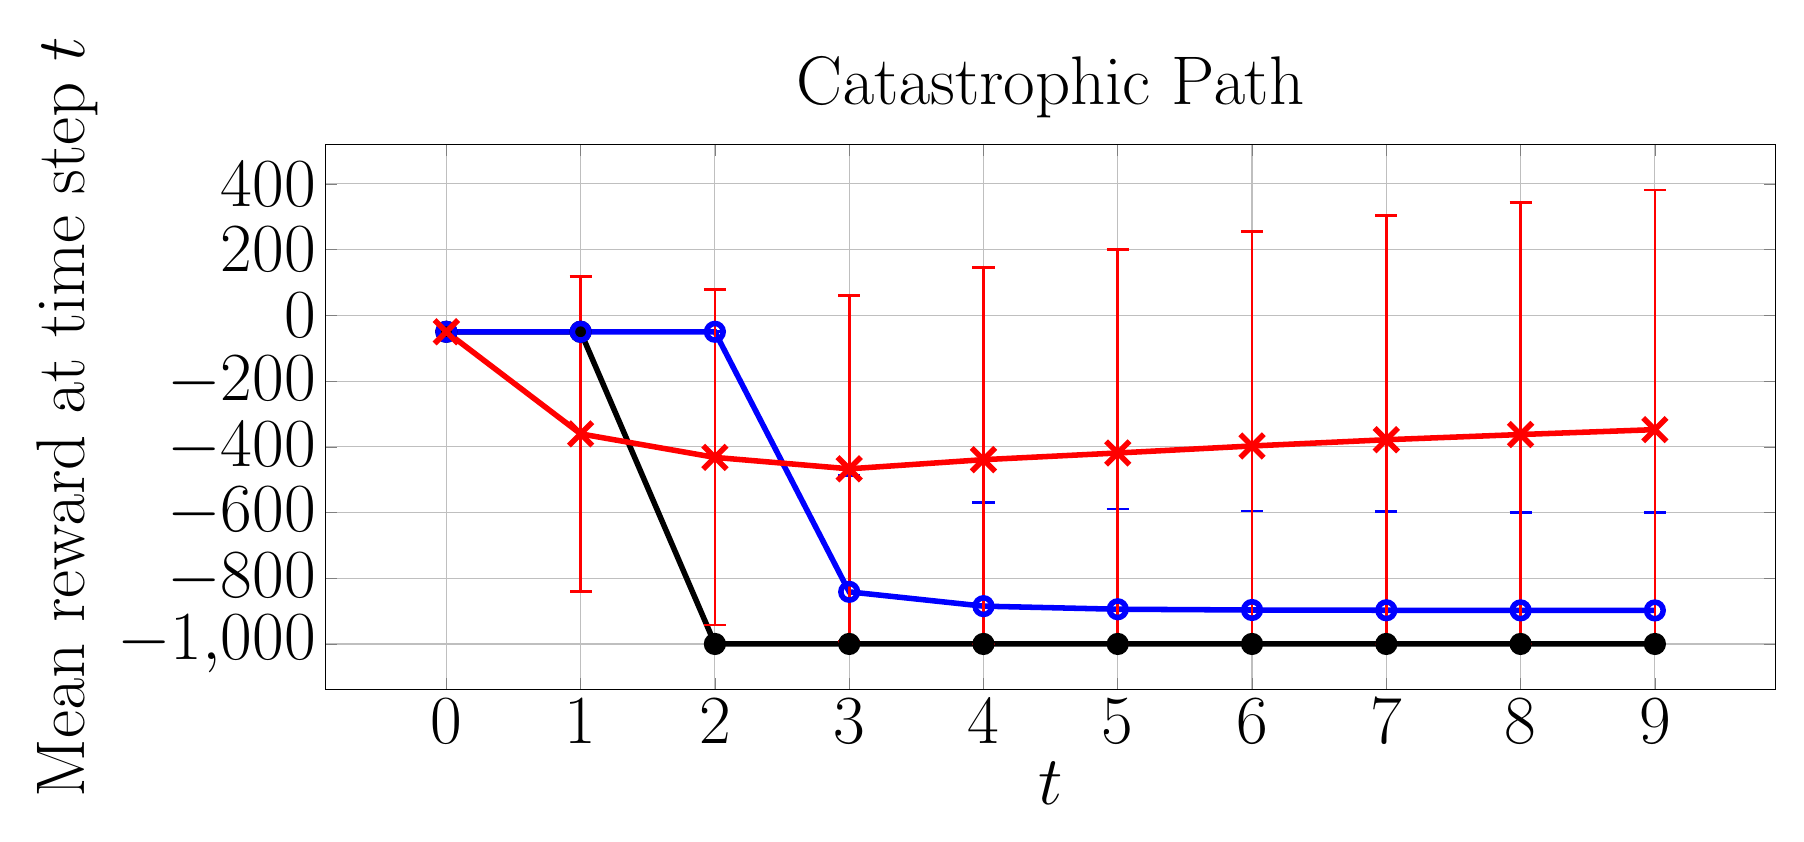
\begin{tikzpicture}
                \begin{axis}[
                    xlabel={$t$},
                    ylabel={Mean reward at time step $t$},
                    title={Catastrophic Path},
                    grid=both,
                    width=20cm, height=8.5cm,
                    every axis/.style={font=\Huge},
                    %
                ]
               \addplot[
                    color=black, %
                    mark=*, %
                    line width=2pt,
                    mark size=3pt,
                ]
                coordinates {
                    (0, -50.0)
                    (1, -50.0)
                    (2, -1000.0)
                    (3, -1000.0)
                    (4, -1000.0)
                    (5, -1000.0)
                    (6, -1000.0)
                    (7, -1000.0)
                    (8, -1000.0)
                    (9, -1000.0)
                };
                %
                %
                \addplot[
                    color=blue, %
                    mark=o, %
                    line width=2pt,
                    mark size=3pt,
                    error bars/.cd,
                    y dir=both, %
                    y explicit, %
                    error bar style={line width=1pt,solid},
                    error mark options={line width=1pt,mark size=4pt,rotate=90}
                ]
                coordinates {
                    (0, -50.0)  +- (0, 0.0)
                    (1, -50.0)  +- (0, 0.0) 
                    (2, -50.0)  +- (0, 0.0) 
                    (3, -841.440725)  += (0, 354.24605512) -= (0, 158.559275)
                    (4, -884.98225)  += (0, 315.37519669) -= (0, 115.01775)
                    (5, -894.330425) += (0, 304.88572805) -= (0, 105.669575)
                    (6, -896.696175) += (0, 301.19954514) -= (0, 103.303825)
                    (7, -897.4635) += (0, 299.61791279) -= (0, 102.5365)
                    (8, -897.77595) += (0, 298.80392585) -= (0, 102.22405)
                    (9, -897.942975) += (0, 298.32920557) -= (0, 102.057025)
                };
                %
                \addplot[
                    color=red, %
                    mark=x, %
                    line width=2pt,
                    mark size=6pt,
                    error bars/.cd,
                    y dir=both, %
                    y explicit, %
                    error bar style={line width=1pt,solid},
                    error mark options={line width=1pt,mark size=4pt,rotate=90}
                ]
            coordinates {
                    (0, -50.0)  +- (0, 0.0)
                    (1, -360.675265)  +- (0, 479.39812699) 
                    (2, -432.27629)  +- (0, 510.38620897) 
                    (3, -467.029545)  += (0, 526.36009628) -= (0, 526.36009628)
                    (4, -439.17429)  += (0, 583.96638919) -= (0, 560.82571)
                    (5, -418.82704) += (0, 618.43027478) -= (0, 581.17296)
                    (6, -397.464895) += (0, 652.67322574) -= (0, 602.535105)
                    (7, -378.49052) += (0, 682.85407033) -= (0, 621.50948)
                    (8, -362.654195) += (0, 707.01412023) -= (0, 637.345805)
                    (9, -347.737935) += (0, 729.29076479) -= (0, 652.262065)
                };
                %
                %
                %
                %
                %
                %
                %
                %
                %
                %
                %
                %
                %
                %
                %
                %
                %
                %
                %
                \end{axis}
            \end{tikzpicture}
         }
    }
    \caption{Average instant reward of CF paths induced by policies on Sepsis.}
    \label{fig: reward sepsis}
\end{figure*}

%
%
%
\subsection{Interval CFMDP Bounds}
%
%
Table \ref{tab:nonzero_probs} presents the mean counterfactual probability bound widths (excluding transitions where the upper bound is $0$) for each MDP, averaged over 20 observed paths. We compare the bounds under counterfactual stability (CS) and monotonicity (M) assumptions, CS alone, and no assumptions. This shows that the assumptions marginally reduce the bound widths, indicating the assumptions tighten the bounds without excluding too many causal models, as intended.
\renewcommand{\arraystretch}{1}

\begin{table}
\centering
\caption{Mean width of counterfactual probability bounds}
\resizebox{0.8\columnwidth}{!}{%
\begin{tabular}{|c|c|c|c|}
\hline
\multirow{2}{*}{\textbf{Environment}} & \multicolumn{3}{c|}{\textbf{Assumptions}} \\ \cline{2-4}
 & \textbf{CS + M} & \textbf{CS} & \textbf{None\tablefootnote{\jl{Equivalent to \citet{li2024probabilities}'s bounds (see Section \ref{sec: equivalence with Li}).}}} \\ \hline
\textbf{GridWorld} ($p=0.9$) & 0.0817 & 0.0977 & 0.100 \\ \hline
\textbf{GridWorld} ($p=0.4$) & 0.552  & 0.638  & 0.646 \\ \hline
\textbf{Sepsis} & 0.138 & 0.140 & 0.140 \\ \hline
\end{tabular}
}
\label{tab:nonzero_probs}
\end{table}


\subsection{Execution Times}
Table \ref{tab: times} compares the average time needed to generate the interval CFMDP vs.\ the Gumbel-max SCM CFMDP for 20 observations.
The GridWorld algorithms were run single-threaded, while the Sepsis experiments were run in parallel.
Generating the interval CFMDP is significantly faster as it uses exact analytical bounds, whereas the Gumbel-max CFMDP requires sampling from the Gumbel distribution to estimate counterfactual transition probabilities. \jl{Since constructing the counterfactual MDP models is the main bottleneck in both approaches, ours is more efficient overall and suitable for larger MDPs.}
\begin{table}
\centering
\caption{Mean execution time to generate CFMDPs}
\resizebox{0.99\columnwidth}{!}{%
\begin{tabular}{|c|c|c|}
\hline
\multirow{2}{*}{\textbf{Environment}} & \multicolumn{2}{c|}{\textbf{Mean Execution Time (s)}} \\ \cline{2-3} 
                                      & \textbf{Interval CFMDP} & \textbf{Gumbel-max CFMDP} \\ \hline
\textbf{GridWorld ($p=0.9$) }                  & 0.261                   & 56.1                      \\ \hline
\textbf{GridWorld ($p=0.4$)  }                 & 0.336                   & 54.5                      \\ \hline
\textbf{Sepsis}                                 & 688                     & 2940                      \\ \hline
\end{tabular}%
}
\label{tab: times}
\end{table}


%%%% DISCUSSION %%%%
\vspace{-0.04in}
\section{Discussion}
\label{sec:discussion}

In this section, we discuss the limitations in current LLM planning research studies, and suggest future directions for improvement and more comprehensive evaluations of LLM planning performance.

\vspace{-0.08in}
\paragraph{Datasets and Baselines} The current evaluation of LLM planning has its limitations, primarily because studies often rely on limited datasets and baselines. This makes it tough to fairly and comprehensively compare different methods. Most studies only use a few datasets from a single domain and difficulty level, and they do not evaluate all the six performance criteria. Inconsistent dataset choices make direct comparisons difficult. On top of that, many studies only compare against basic baselines such as CoT or ReAct, which does not help in comparing more advanced approaches. To fix this, a public, standardized leaderboard should be set up that covers all performance criteria, uses consistent evaluation metrics, includes a variety of baseline and advanced methods, and utilizes diverse datasets spanning multiple domains and difficulty levels. Another useful direction would be to create multilingual planning datasets and assess LLM performance across different languages.

\vspace{-0.08in}
\paragraph{Representation}\; LLMs are highly sensitive to prompts \cite{sclar2024quantifyinglanguagemodelssensitivity, razavi2025benchmarkingpromptsensitivitylarge}, but most research relies on natural language without comparing them to alternative formats, such as PDDL or Python, for describing domains and problems. Some studies \cite{singh2023progprompt, aghzal2024look} suggest that using Python to represent planning problems can improve performance, but automatically translating natural language problem descriptions into Python remains challenging, particularly for non-experts. If LLMs are to handle this translation effectively, additional datasets and evaluations are needed to assess their performance. Furthermore, little research has been conducted on how different prompt templates impact LLM planning performance, or on the best output formats for representing plans. Lastly, most fine-tuning methods rely on natural language data without exploring other formats, such as symbolic representations. Filling these gaps requires building benchmarks like Planetarium \cite{zuo2024planetarium} and carefully choosing representation formats in experiments.

\vspace{-0.08in}
%\vspace{-0.07in}
%\vspace{-0.05in}
\paragraph{Hallucination}  LLMs often experience hallucinations \cite{huang2023survey}, which present two major challenges in planning. First, they might struggle to assess if a plan is achievable given a specific problem description \cite{aghzal2023can, kambhampati2024can}. Second, they can generate inadmissible actions and non-existent objects, requiring translation or expert intervention to correct them \cite{huang2022language, raman2022planning}. This increases the cost of planning systems. Further research is needed to understand the root causes and improve LLMs' ability to accurately identify unachievable plans. Evaluating the impact of these hallucinations remains an important research direction.

\vspace{-0.08in}
%\vspace{-0.07in}
%\vspace{-0.05in}
\paragraph{Human Preference Alignment}\; There is a gap in understanding whether system generated plans align with human preferences. It is crucial for open-ended problems where humans execute the plans. Ensuring alignment with human preferences is vital for safety, feasibility, and usability, particularly in personalized planning tasks such as calendar and travel planning. Additionally, \citet{aghzal2024look} found that LLM planners often fail to achieve optimality in path planning, frequently producing unnecessarily long plans. This may stem from inherent length bias in LLMs, which tend to generate longer sequences. Alignment techniques such as RLHF \cite{ouyang2022training} and DPO \cite{rafailov2024direct} may help alleviate this issue, as humans generally prefer shorter plans for their efficiency, simplicity, and cognitive ease. Further investigation is needed to better align LLM planners with human preferences.

\vspace{-0.07in}
%\vspace{-0.05in}
\paragraph{Cost Effectiveness} Current methods, particularly task decomposition and search-based approaches, often consume a large number of tokens due to lengthy prompts and repeated LLM queries. While heuristic search is considered more efficient than task decomposition, it still requires substantial repeated prompting. To improve cost-effectiveness, we may summarize problem descriptions and enhance heuristic evaluations, e.g., by improving LLM uncertainty estimation \cite{huang2024survey} and verification \cite{li2024systematicanalysisllmcontributions}. These improvements would help reduce prompt length and enable the early stopping of unpromising partial plans.

\vspace{-0.07in}
%\vspace{-0.05in}
\paragraph{Multi-Agent Planning} Most existing research focuses on single-agent planning, where only one agent performs a task. Multi-agent planning \cite{konolige1980multiple, torreno2017cooperative} is more challenging, as it involves multiple agents (e.g., robots) working together or competing in parallel. Despite its complexity, multi-agent planning has received limited attention in AI planning research. It often requires coordinating multiple agents in collaborative or competitive environments where they operate simultaneously. The major challenge lies in developing effective communication protocols and cooperation strategies while generating viable plans for their collective actions.

\vspace{-0.07in}
%\vspace{-0.05in}
\paragraph{Reasoning, Tool Use, and Memory}\quad There is often limited discussion on how other components of LLM agents, such as reasoning, tool use, and memory, affect planning performance. In particular, when LLMs are combined with classical planners or optimizers, it is crucial that the LLM accurately translates the planning problem into the appropriate domain representation to ensure correct plan generation. Currently, these approaches rely on human-selected planners and optimizers. Treating them as tools that LLMs can autonomously choose from could be an exciting prospect. This also raises the question of whether LLMs can effectively select the best tool for a given planning task. Future research should look into enhancing these agentic capabilities in LLM-based planning.




%In this section, we discuss limitations of the current LLM planning work and point out future directions to further enhance and more comprehensively evaluate the LLM planning performance. \hwnote{Need to make the logic in the following paragraphs correct.} 

% The current evaluation of LLM planning is insufficient, due to the limited datasets and baselines used in each study, making it difficult to comprehensively and fairly compare different proposed methods. First of all, most studies use a limited number of datasets with a single domain and difficulty level, and none of them evaluates all six aforementioned performance criteria. Inconsistent datasets choices further hinder direct and fair comparisons. Second of all, many studies only compare against basic baselines, such as CoT and ReAct, making it hard to directly compare more advanced approaches from their reported results. To address these issues, a public, standardized leaderboard should be established. It should incorporate all performance criteria, consistent evaluation metrics, a range of baseline and advanced methods, as well as diverse datasets covering multiple domains, difficulty levels. Another direction is to create multilingual planning datasets and assess LLM performance across languages.%\smallskip

% There is no benchmark that comprehensively evaluates LLM-based planners across all aforementioned six performance criteria. Additionally, most of the examined studies use a limited number of datasets within a single domain and difficulty level. As a result, the reported findings fail to capture all the limitations of the proposed methods, making it challenging for practitioners to select the most suitable approach for their specific needs. Moreover, differences in datasets across studies hinder direct and fair comparisons. Furthermore, many works rely on basic baseline models, such as CoT and ReAct, making it difficult to compare more advanced approaches. Moving forward, a public leaderboard should be established, incorporating all six performance criteria, standardized evaluation metrics, both classical and advanced baseline models, and diverse datasets spanning multiple domains and difficulty levels. \smallskip

% There is no benchmark to comprehensively test LLM-based planners with all the aforementioned six performance criteria. Also, most of the work in the examined papers are using limited number of datasets within a single domain and single difficulty. Thus, the reported results cannot reveal all the limitations of the proposed methods, making it hard for the practitioners to choose which one to use based on their specific needs. Also, Their datasets are also different from other work, making them difficult to compare them directly and fairly. Furthermore, most of the work have very basic baseline models, such as CoT and ReAct, which makes it difficult to compare these more advanced work with each other. In the future, there should be a public leaderboard, with all the six performance criteria, standardized evaluation metrics, both classical and advanced baseline models, and diverse datasets with multiple difficulty and domains. 

% No unified baseline models. Baselines from most of the papers are CoT, ReAct, and ToT, with no advanced developed methods surveyed by this paper.

% Although there are some benchmarks [Embodied interface, PPNL] which target multiple criteria, the datasets and the tasks contained in the benchmark are not diverse enough. 



% The current investigation of input, output, and fine-tuning data representation is insufficient. LLMs are highly sensitive to prompts \cite{sclar2024quantifyinglanguagemodelssensitivity, razavi2025benchmarkingpromptsensitivitylarge}, yet most studies rely solely on natural language representations without comparing alternative formats such as PDDL or Python for describing domains and problems. Some research \cite{singh2023progprompt, aghzal2024look} suggests that using Python to represent problems can improve performance, but the challenge of automatically translating natural language instructions into Python, especially for non-experts, remains unresolved. If LLMs are to be used for this translation, additional datasets and evaluations are needed to assess their effectiveness. Additionally, no studies have explored how different prompt templates affect LLM-based planning performance. Similarly, there is little discussion on the choice of output formats for representing plans, and it remains unclear whether output representation affects planning performance. Finally, most fine-tuning-based methods rely on natural language data without exploring other formats, such as symbolic representations. Addressing these gaps requires both constructing benchmarks like Planetarium \cite{zuo2024planetarium} and carefully selecting representation formats in experiments.

% The current investigation of representation of inputs, outputs and fine-tuning data are not sufficient. LLMs are highly sensitive to prompts \cite{sclar2024quantifyinglanguagemodelssensitivity, razavi2025benchmarkingpromptsensitivitylarge}, yet most studies rely on natural language representations without comparing alternative formats, such as PDDL or Python, for describing domains and problems. Some research \cite{singh2023progprompt, aghzal2024look} suggests that representing problems with Python code can improve performance, but the challenge of translating natural language instructions into Python automatically remains unresolved. If LLMs are to be used for this translation, additional datasets and evaluation are needed to explore their effectiveness. Furthermore, no studies have examined how different prompt templates impact LLM-based planning performance. Similarly, there is little discussion on the choice of output formats for representing plans, and it remains unclear whether output representation affects planning performance. Finally, most of fine-tuning work are using data of natrual language, without explore other formats, such as symbolic representation. All these unknowns deserve further investigation by both constructing the benchmarks like Planetarium \cite{zuo2024planetarium} and carefully choose representation formats during experiments. \smallskip
% LLMs are known sensitive to the prompts. However, most of the work are using natural language representation instead of comparing different representations (such as PDDL, Python) to describe the domain and problems on their tasks. Also, some work found representing plans with Python code can improve the performances, but they did not clearly solve the problem how to convert the natural language instructions into these python code. If we can resort to LLMs, more datasets needs to be developed to test this translation ability. Also, no work discusses the impact of different prompt templates to the performance of the LLM planning. Similar to the inputs, there is no work talking about which output formats should be chosen to represent the plans. It is even unknown if the output representation can actually affect the planning performance. \smallskip

% Inputs (Prompt): 
% What format is the best way to represent the (different) problems? PDDL? Python code? There are only a few studies discussing this (e.g., [Aghzal 2024] for path planning).
% What prompt templates to choose? Since LLMs are very sensitive to the prompt templates, different prompt templates might have different planning performance. 
% If the LLMs can perform better by using formal representation to describe the problem [Aghzal 2024, Pallagani 2023], how should we convert the natural language into these formal representations for non-experts? Can we use another LLM to translate them? How are their performance ⇒ Need more datasets to test this, (e.g. Planetarium [Zuo et al.] for PDDL, but what about other formats, such as Python code?)% Outputs: 



% LLMs suffer from hallucination \cite{huang2023survey}, creating two major challenges in LLM-based planning. First, they struggle to determine whether a given problem is achievable \cite{aghzal2023can, kambhampati2024can}. Second, they generate inadmissible actions and non-existent objects in plans, which needs extra translation and corrections and reduce the efficiency of the planning system \cite{huang2022language, raman2022planning}. Further research is needed to understand the underlying causes of these issues and improve LLM-based planning ability to accurately identify unachievable problems. Additionally, further evaluating the impact of hallucinations on LLM planning remains an important research direction.

%How to further evaluate the hallucination impact on LLM planning is another direction. %\smallskip
% It is known that LLMs suffer from hallucination. In terms of the LLM planning, it causes two problems: fail to identify the achievability of an given problem [Aghzal 2024, ASU o1 paper], and generate nonadmissble actions and non-existing objects in the plans [Huang 2022, Raman 2023]. There is more work to do to investigate why and how these could happen. Also, improving the LLM planning for identifying the unachievable problems is an very important problem.  


% While current LLM planning research focuses on standard evaluation metrics, no work has examined whether the generated plans align with human preferences. This is a crucial question, especially for open-ended problems where humans execute the plans. Ensuring alignment with human preferences is essential for safety, feasibility, and usability. This issue is particularly relevant for personalized planning tasks, such as scheduling (e.g., calendar and travel planning). Additionally, \citet{aghzal2024look} found that LLM-based planners fail to achieve optimality in path-planning problems, often producing unnecessarily long plans. This may stem from an inherent length bias in LLMs, which tend to generate longer sequences. Alignment techniques like RLHF \cite{ouyang2022training} and DPO \cite{rafailov2024direct} could help address this issue, as humans generally prefer shorter plans for their efficiency, simplicity, and cognitive ease. Further investigate is needed for these issues and better align LLM-based planners with human preferences.

% Although the current LLM planning is focusing on the aforementioned evaluation metrics, there is no work focusing on if the output plans are preferred by humans. This is a very important question, especially when the problem is open-ended and the executors are human beings. Also, aligning with Human preference is necessary to make sure all the steps are safe and secure and executable to conduct. Also, this problem is very important to do the personalization planning, especially for task scheduling (e.g., calendar and travel planning). Furthermore, \citet{aghzal2024look} demonstrates that LLM planner cannot achieve the optimality on the path planning problems, ending with outputting unnecessarily long plans. This might be due to the internal length bias of the LLMs, which is they prefer to generate longer sequences than shorter ones. So alignment approaches, such as RLHF and DPO, might be the solution to solve this problem since humans generally prefer shorter plans due to cognitive ease, efficiency, and reduced complexity. \smallskip





% Current approaches, especially task decomposition and search-based methods, often requires significant token consumption due to lengthy prompts and repeated queries. To further improve efficiency, more compact problem descriptions and better heuristic evaluations (e.g., improved LLM uncertainty estimation \cite{huang2024survey} and LLM-verification \cite{li2024systematicanalysisllmcontributions}) should be introduced, which would reduce prompt lengths and enable early-stopping of unpromising partial plans. 

% , also, it is important to excel across many tasks but still faces efficiency bottlenecks. Approaches  How to design better heuristic score function (e.g., model better uncertain) and do the early stopping needs the future investigation. \hwnote{Althgouth heuristic search are more efficient than task decomposition, they still involves hugh amount of repeated prompting.} \smallskip



% Multi-agent planning \cite{konolige1980multiple, torreno2017cooperative}, a classical and more complex AI planning problem, has received limited attention in LLM planning research. Unlike single-agent scenarios, multi-agent planning involves coordinating multiple agents (e.g., robots) that can operate simultaneously and independently. The challenge lies in developing effective cooperation and communication protocols among these agents while generating viable plans for their collective actions.

%Multi-agent planning is a classical problems in the AI planning field, which are very rarely discussed by LLM planning studies. Multiple-agent planning involves multiple agents (e.g., robots) which can operate in parallel and independently, how to make them cooperate and communicate with each other, and plan for this scenario is more challenging than current single-agent scenarios.

% However, most of the examined work are focused on single-agent planning, which means we only plan for one agent (e.g. one robot). Since multiple agents can operate in parallel independently, how to make them cooperate and communicate with each other is more challenging. \smallskip 



% There is limited discussion on how other LLM agent components (i.e., reasoning, tool usage, and memory) impact planning performance. Additionally, while combining LLMs with classical planners or optimizers can ensure correct plan generation if the LLM's translation is accurate, these approaches rely on human-selected planners and optimizers. Treating external planners and optimizers as tools that LLMs can autonomously choose raises the question of whether LLMs can select the most suitable tool based on the given planning problem. Future research should explore improving LLM-based planning by enhancing these agentic capabilities.

% There are limited discussion about the impact of other LLM agent components (i.e., reasoning, tool-use and memory) on its planning abilities. Additionally, although LLM + classical planner / optimizer can guarantee to generate the correct plan if the LLM translation are correct, these work rely on human preselected planners and optimizers. If we consider external planners and optimizers as the external tools which can be used by LLMs, there is more evaluation to see if LLMs can automatically select the appropriate tools based on the planning problems given to them. Thus, the future research can also explore the direction to improving the LLM planning by enhancing other agentic abilities.

%Secondly, there is limited discussion about if improved reasoning abilities and extra internal and external memory can improve the LLM planning abilities. Thus, the future resaerch can also explore the direction to improving the LLM planning by enhancing other agentic abilities.


% First of all, planning requires reasoning abilities, however, there are not a lot of work verifying this and which reasoning methods are the best for LLM planning, given the fact that the most commonly-used reasoning method (i.e., CoT) have limited improvement in limited scenarios. Secondly,  Lastly, like reasoning, there is not a lot of work discussing about the impact of both internal and external memory for the LLM planning abilities. In the future, 

% Firstly, CoT is the most commonly-used reasoning method used in the LLM planning tasks. However, there is no discussion about if this is the best way for LLM planning given the fact that CoT only improves the performance when the human demonstra \citet{} 

% % planning needs reasoning, reasoning and planning are intertwined, which means enhancing reasoning abilities can also improve the planning abilities. However, there is not a lot of work illustrating this. So in the future, we can also test which reasoning methods we should use. Currently, the most common way to do this is CoT and [Stechly 2024] demonstrates the CoT might only depend on a specific prompt engineering to achieve the improvement on the planning tasks. 

% % Reasoning:
% % Since reasoning and planning are intertwined, which means enhancing reasoning abilities can also improve the planning abilities. However, there is not a lot of work illustrating this. So in the future, we can also test which reasoning methods we should use. Currently, the most common way to do this is CoT and [Stechly 2024] demonstrates the CoT might only depend on a specific prompt engineering to achieve the improvement on the planning tasks. 
% External tools:
% When discussing LLM + Classical Planners / Optimizer, no paper is talking about why the specific classical planner or optimizer is used. If we consider these planners and optimizers as a tool, then can LLM automatically choose the optimal or suitable one to use? And also which representation to use? All these are to achieve the fully automatic planning system. 
% Memory
% Although some work exploring the impact of LLM memory for the planning ability, there should be more work exploring this area. Some work talking about this (they talk about how to store the learned successful and failure trajectories and experiences in the memory and facilitate the future planning): “Large Language Models Are Semi-ParametricReinforcement Learning Agents”, “Agent Planning with World Knowledge Mode”.

%\paragraph{Multilingual}






%%%% CONCLUSION %%%%
\section{Conclusion}
% In conclusion, this study highlights the efficacy and potential of integrating Parameter-Efficient Fine-Tuning (PEFT) methods with game theory principles through the innovative approach of LoRA with Mixture of Gamers (\ourmethod). By melding Low-Rank Adaptation (LoRA) with Mixture of Experts (MoE) and utilizing game theory-based dynamics, \ourmethod{} significantly advances the field by addressing critical gaps in flexibility and dynamic expert selection inherent in previous methods. The employment of submatrix decomposition alongside Shapley values in \ourmethod{} enables a more granular understanding of the interactions and contributions of different components within PEFT setups. The promising experimental outcomes across a variety of tasks not only underscore \ourmethod's superior performance but also illuminate its versatile applicability and the potential for future adaptations in complex, domain-specific applications. Moving forward, it will be crucial to refine these approaches, ensuring robustness and scalability, to fully harness the transformative power of PEFT in enhancing machine learning models.

In this paper, we introduce \ourmethod{}, a Med-LVLM that unifies medical vision-language comprehension and generation through a novel heterogeneous knowledge adaptation approach.
% integrates H-LoRA and a three-stage fine-tuning approach, aim at unifying medical understanding and generation tasks. 
% To enhance the multi-task performance of \ourmethod{}, we introduce the \texttt{VL-Health} dataset for training. 
Experimental results demonstrate that \ourmethod{} achieves significant performance improvements across multiple medical comprehension and generation tasks, showcasing its potential for healthcare applications. 

%%%% LIMITATION %%%%
\section{Limitations} \label{sec:limitation}

This work primarily focuses on commonly studied domains involving single-agent scenarios, such as robotics, household tasks, and computer-based tasks. We acknowledge that LLM planning is also applied in other areas, including the natural sciences \cite{o2023bioplanner, liu2024multimodal}, the Internet of Things \cite{cui2024llmind}, and multi-agent scenarios. However, these studies follow similar methodologies and evaluations, suggesting our survey's comprehensiveness. We focus on six commonly used performance criteria and exclude others, such as security and personalization, due to limited research in these areas. Instead, we discuss them in our future directions section.


% Bibliography entries for the entire Anthology, followed by custom entries
%\bibliography{anthology,custom}
% Custom bibliography entries only
\bibliography{custom}

\section{Theoretical Analysis}
\subsection{Notations}
We dedicate Table~\ref{tab:Notation} to index the notations used in this paper. Note that every notation is also defined when it is introduced.
\begin{table*}[h!]
\caption{Notations.}\label{tab:Notation}%\\
\centering  
% \resizebox{\textwidth}{!}{
\begin{tabular}{l l l}
\toprule
 $\gG$ &$\triangleq$ & Input graph with a vertex set $\gV$, an edge set $\gE$, and features $\mX$\\
 $\boldsymbol{A}$ &$\triangleq$ & Adjacency matrix of $\gG$\\
 $\gE$ & $\triangleq$ & Edges of $\gG$\\
 $\gV$ & $\triangleq$ & Nodes of $\gG$\\
 $\mX$ & $\triangleq$ & Matrix containing node features of $\gG$\\
 $\vy$ & $\triangleq$ & Vector of node labels of $\gG$\\
 $C$ & $\triangleq$ & An ordered set containing all possible node labels of $\gG$\\
 $F$ & $\triangleq$ & Dimension of node features in $\gG$\\
 $L$ & $\triangleq$ & Number of GNN layers\\
 $H$ & $\triangleq$ & Node embedding dimension\\ 
 ${\mH}$ & $\triangleq$ & Node embedding matrix\\
 $\vh_u$ & $\triangleq$ & Embedding of node u\\
 $\vw$ & $\triangleq$ & Vector of edge weights in  $\gG$\\
 $q$ & $\triangleq$ & Ratio of \# edges in sparse graph and \# edges in input graph in \%\\
 $k$ & $\triangleq$ & \# edges in the sparse graph, $k\triangleq\floor{\frac{q|\gE|}{100}}$\\ 
 $\tilde{p}$ & $\triangleq$ & Learned probability distribution by \sgs \\
 $\tilde{\gE}$ & $\triangleq$ & Set of edges sampled from $\gE$ by \sgs following $\tilde{p}$\\
$\tilde{\gG}$ &$\triangleq$ & Sparse subgraph $(\gV,\tilde{\gE},\mX)$ constructed by \sgs \\  
 $\mA_{\tilde{\gG}}$ or $\tmA$ & $\triangleq$ & Adjacency matrix of $\tilde{\gG}$\\
 $\tilde{\vw}$ & $\triangleq$ & Edge weight of sparse graph learned by \sgs \\
 $p_\mathrm{prior}$ & $\triangleq$ & Probability distribution of a fixed prior on $\gG$ \\
  $\tilde{p}_a$ & $\triangleq$ & Augmented learned probability distribution  \\
 $p^*$ & $\triangleq$ & True probability distribution known by the idealized learning ORACLE\\
 ${\gE^*}$ & $\triangleq$ & Set of edges sampled from $\gE$ by the learning ORACLE following distribution $p^*$\\   
 $\gG^*$ &$\triangleq$ & True sparse subgraph $(\gV,\gE^*,\mX)$ constructed by the learning ORACLE \\
 $\mA_{\gG^*}$ or $\mA^*$ & $\triangleq$ & Adjacency matrix of $\gG^*$\\
 % $\gG^*$ &$\triangleq$ & True sparse subgraph constructed by the idealized learning ORACLE \\
 % $\mA_{\gG^*}$ or $\mA^*$ & $\triangleq$ & Adjacency matrix of $\gG^*$\\
 $\gL_\mathrm{CE}$ & $\triangleq$ & Cross entropy loss\\
 $\gL_\mathrm{assor}$ & $\triangleq$ & Assortative loss\\
 $\gL_\mathrm{cons}$ & $\triangleq$ & Consistency loss\\
$\gL$ & $\triangleq$ & Total loss\\ 
 
 
 
 
 
 
 \bottomrule
\end{tabular}
% }
\end{table*}
\subsection{Bounding \#common edges wrt. true subgraph}
\label{theo:commonedges}
Let $\mathcal{E}^*$ and $\mathcal{\tilde{E}}$ denote the ordered collection of edges sampled by the idealized learning ORACLE according to true distribution $p^*$ and by \sgs according to learned probability $\tilde{p}$ respectively. For analytical convenience, let us assume that both learning algorithms sample $k = \floor{q|\mathcal{E}|/100}$ edges with replacement independently.
 
% We will first show that $\mathbf{Pr}(\mathcal{E}_i^* = \mathcal{\tilde{E}}_i) \geq \min_j (p^*_i, \tilde{p}_i)$ and $\min(p^*_i,\tilde{p}_i) = 1- \frac{1}{2} \|\tilde{p} - p^*\|_1$. These two results will lead us to prove that $\mathbf{Pr}(\mathcal{E}_i^* = \mathcal{\tilde{E}}_i) \geq 1 - \frac{\epsilon}{2}$. 
First, we will prove lemma~\ref{lem:singleedge}, which show that the probability of an edge chosen by \sgs coincides with that chosen by the ORACLE has a lower bound. Finally, we will prove one of the main results (Theorem~\ref{theo:commonedges}), which shows that given $q \in [0,100]$, we can lower-bound the expected number of common edges between \sgs and the learning ORACLE. 

\begin{lemma} 
\label{lem:singleedge}
For any arbitrarily chosen $i \in \{1,2,\ldots, k\}$
\[
\mathbf{Pr}(\mathcal{E}_i^* = \mathcal{\tilde{E}}_i) \geq \sum_{j=1}^{|\mathcal{E}|} \frac{(p^*_j + \tilde{p}_j - \epsilon)^2}{4},
\]
where $k = \floor{q|\mathcal{E}|/100}$ and $0 \leq q \leq 100$ is a user-specified parameter and $\epsilon\in [0,1]$ is the error.
\end{lemma}

\begin{proof} We prove the above lemma in two parts.


\paragraph{Part 1: Universal approximation of probability distribution over edges.}
%\label{tho:uap}
The Universal Approximation Theorem~\cite{cybenko1989approximation,augustine2024survey} states that a feed-forward neural network with at least one hidden layer and a finite number of neurons can approximate any continuous function $f: \mathbb{R}^n \rightarrow \mathbb{R}$ on a compact subset of $\mathbb{R}^n$, given a suitable choice of weights and activation functions. 

In our case, $p^* = f$ is the true edge probability distribution for the downstream task, $\tilde{p} = f_{\text{MLP},\phi}$ is the learned approximate distribution and $\vx_e$ is a vector of edge features, for instance, $\vx_e =  ((\vh_u - \vh_v) \oplus (\vh_u \odot \vh_v))$ as used in equation~\ref{eq:w_uv}. The following universal approximation property holds for the module I component of \sgs,
\begin{equation}
\label{eq:uapp}
\sup_{e \in \mathcal{E}} \|\tilde{p}(\vx_e) - p^*(\vx_e)\|_1 \leq \epsilon.
\end{equation}
 Here, we have two underlying assumptions: (i) the optimal distribution $p^*$ is a function of node features $\mX$ and (ii) $\mX$ is a compact subset (bounded and closed) of Euclidean space $\mathbb{R}^n$. The first assumption is made to simplify the problem. The second assumption is quite practical since the node features are typically normalized. Hence, we can show that the embeddings $\vh_u,\vh_v$, which are continuous images of $\mX$, are also compact due to the extreme value theorem. As a result, the edge features $\vx_e$ which, in a sense, \emph{lifts} the end-point node features into higher-dimensional Euclidean space are also compact. The approximation error $\epsilon$ can be made arbitrarily small by increasing the capacity of the MLP, e.g., adding more neurons or layers. 

\paragraph{Part 2: Common edges wrt. optimal subgraph.}

The event $\mathcal{E}_i^* = \mathcal{\tilde{E}}_i$ means that both $\mathcal{E}_i^*$ and $\mathcal{\tilde{E}}_i$ contain the same edge. But there are $|\mathcal{E}|$ such candidates. Hence, the probability of this event is given by,

\begin{align*}
    \mathbf{Pr}(\mathcal{E}_i^* = \mathcal{\tilde{E}}_i) &= \sum_{j=1}^{|\mathcal{E}|} \mathbf{Pr}(\mathcal{E}_i^* = \mathcal{E}_j \land \mathcal{\tilde{E}}_i = \mathcal{E}_j), \\
    &= \sum_{j=1}^{|\mathcal{E}|} \mathbf{Pr}(\mathcal{E}_i^* = \mathcal{E}_j) \cdot \mathbf{Pr}(\mathcal{\tilde{E}}_i = \mathcal{E}_j), \\
    & = \sum_{j=1}^{|\mathcal{E}|} p^*_j \cdot \tilde{p}_j, \\
    &\geq \sum_{j=1}^{|\mathcal{E}|} \frac{(p^*_j + \tilde{p}_j - |p^*_j - \tilde{p}_j|)^2}{4}, \\
    & \geq \sum_{j=1}^{|\mathcal{E}|} \frac{(p^*_j + \tilde{p}_j - \epsilon)^2}{4}.
\end{align*}
The second line follows since the optimal sampler is a different algorithm independent from the sampler used in \sgs. The last line follows because $\|p^*_j - \tilde{p}_j\|_1 \leq \epsilon \implies |p^*_j - \tilde{p}_j| \leq \epsilon$ (from eq.~\ref{eq:uapp}). 
\end{proof}

% \begin{lemma}
% \[
%     \min(p^*_i,\tilde{p}_i) = 1- \frac{1}{2} \|\tilde{p} - p^*\|_1
% \]
% \end{lemma}
% \begin{proof}
%     It is known (for instance, see~\cite{xie2024distributionally}) that the total variation distance $d_{TV}(\tilde{p},p^*)$ satisfies
%     \[
%     d_{TV}(\tilde{p},p^*) = \frac{1}{2}\|\tilde{p} - p^*\|_1
%     = 1 - \min({\tilde{p},p^*})
%     \]
% \end{proof}

We have the following theorem that lower-bounds the number of common edges with respect to the optimal sampler $|\mathcal{E} ^* \cap \mathcal{\tilde{E}}|$: 
\begin{theorem}[Lower-bound]
\begin{equation}
\mathbb{E}[|\mathcal{E}^* \cap \mathcal{\tilde{E}}|] \geq k \sum_{j=1}^{|\mathcal{E}|} \frac{(p^*_j + \tilde{p}_j - \epsilon)^2}{4},
\end{equation}
where $k = \floor{q|\mathcal{E}|/100}$ and $0 \leq q \leq 100$ is a user-specified parameter.
\end{theorem}
\begin{proof}
    Since we are drawing $k$ edges independently at random, the theorem follows by applying the linearity of expectation on the following:
\begin{align*}
\mathbb{E}[|\mathcal{E}^* \cap \mathcal{\tilde{E}}|] = \mathbb{E}[\sum_{i=1}^k \mathbb{I}(\mathcal{E}_i^* = \mathcal{\tilde{E}}_i)] &= \sum_{i=1}^k \mathbf{Pr}(\mathcal{E}_i^* = \mathcal{\tilde{E}}_i) \\
& = k\cdot \mathbf{Pr}(\mathcal{E}_i^* = \mathcal{\tilde{E}}_i)\\
& \geq k \sum_{j=1}^{|\mathcal{E}|} \frac{(p^*_j + \tilde{p}_j - \epsilon)^2}{4}
\end{align*}
\end{proof}
This theorem shows that the expected number of common edges between the sample subgraph obtained by \sgs $\mathcal{\tilde{G}}$ and the true optimal sample subgraph $\mathcal{G}^*$ is non-trivial. 

% \paragraph{The implication of the lower-bound.} 
% (1) Suppose, the true distribution is uniform. In the best case scenario $\epsilon \rightarrow 0$ and $\tilde{p} = p^* = \frac{1}{|\mathcal{E}|}$. Thus there are at least $\frac{k}{|\mathcal{E}|}$ common edges between $\tilde{\gG}$ and $\gG^*$. However, since $k < \abs{\mathcal{E}}$, the lower-bound of $\mathbb{E}[|\mathcal{E}^* \cap \mathcal{\tilde{E}}|] \geq \frac{k}{|\mathcal{E}|}$ is not very useful even though the learned distribution is accurate. This suggests that \emph{learning the optimum uniform distribution is less likely to produce the optimum sparse subgraph}. 

% (2) Suppose, the true distribution is the Dirac distribution (often called the $\delta$ distribution) where all probability mass is concentrated on a single edge. In other words, suppose $\tilde{p} = p^* = \delta_{ij}$ where $\delta_{ij}$ is the Kronecker-delta. In such a skewed distribution, as $\epsilon \rightarrow 0$, the lower bound reduces to 
% \[
% \mathbb{E}[|\mathcal{E}^* \cap \mathcal{\tilde{E}}|] \geq k \sum_{j=1}^{|\mathcal{E}|} (\tilde{p}_j)^2 = k.
% \]
% This identity suggests that the sampled edges are expected to 100\% overlap with the true, optimal sparse subgraph.

\begin{theorem}[Upper-bound]
\begin{equation}
\mathbb{E}[|\mathcal{E}^* \cap \mathcal{\tilde{E}}|] \leq k (1 - \frac{\|p^* - \tilde{p}\|_1}{2}), 
\end{equation}
where $k = \floor{q|\mathcal{E}|/100}$ and $0 \leq q \leq 100$ is a user-specified parameter.
\end{theorem}
\begin{proof}
\begin{align*}
    \mathbf{Pr}(\mathcal{E}_i^* = \mathcal{\tilde{E}}_i) &= \sum_{j=1}^{|\mathcal{E}|} p^*_j \cdot \tilde{p}_j \\
    & \leq \sum_{j=1}^{|\mathcal{E}|} \min(p^*_j,\tilde{p}_j) \\
    &= 1 - d_{TV}(p^*,\tilde{p}) \\
    &= 1 - \frac{1}{2} \|p^* - \tilde{p}\|_1    
\end{align*}
\end{proof}
Here $d_{TV}$ is the total variation distance. The result used in the last line regarding $d_{TV}$ can be found in~\citet{xie2024distributionally}. 

\paragraph{The implication of the upper-bound.} 
When $\tilde{p} \rightarrow p^*$, the norm $\|p^* - \tilde{p}\|_1 \rightarrow 0$; therefore, the number of common edges could be close to $k$.

\subsection{Upper-bounding the error in the learned Adjacency matrix} 
With the bound proven earlier on the \#common edges by the sparse subgraph of \sgs with that by a learning ORACLE, in this section, we want to obtain an upper-bound on the error in terms of the norm of the Adjacency matrices. As adjacency matrices are used by GNNs for computing node embeddings, such result is important for obtaining error bound on the embeddings later on.

Let $\mA_{\tilde{\gG}}$ and $\mA_{\gG^*}$ be the corresponding adjacency matrices of the learned sparse graph $\tilde{\gG}$ and true optimal sparse graph $\gG^*$. The dimension of these matrices is the same as the input adjacency matrix $\mA_{\mathcal{G}}$ except that $\mA_{\mathcal{G}}$ is denser. Let us also denote the Frobenius norm of a matrix $\mA$ as $\|\mA\|_F$ and the spectral norm of $\mA$ as $\|\mA\|_2$. The Frobenius norm of $\mA$ is defined as $\sqrt{\sum_{ij} \mA^2_{ij}}$, whereas the spectral norm of $\mA$ is the largest singular value $\sigma_{max}(\mA)$ of $\mA$.


Since \sgs do not know the true probability distribution $p^*$, error is introduced in the learned adjacency matrix $\mA_{\tilde{\gG}}$ of the downstream sparse subgraph. We are interested in analyzing the expected error introduced in $\mA_{\tilde{\gG}}$ in terms of the spectral norm, to be precise, $\mathbb{E}[\|\mA_{\tilde{\gG}} - \mA_{\gG^*}\|_2]$. To this end, we will exploit the lower bound derived in Theorem 1 and the fact that $\|\mA\|_2 \leq \|\mA\|_F$. 

\begin{lemma}[Error in Adjacency matrix approximation] Let $\mA_{\tilde{\gG}}$ and $\mA_{\gG^*}$ be the corresponding adjacency matrices of the learned sparse graph $\tilde{\gG}$ and true optimal sparse graph $\gG^*$. If the downstream sampler sampled $k$ edges independently at random (with replacement) to construct those matrices following their respective distributions $\tilde{p}$ and $p^*$, then 
    \[
    \mathbb{E}[\|\mA_{\tilde{\gG}} - \mA_{\gG^*}\|_2] \leq \sqrt{2k(1-\sum_{j=1}^{\abs{\mathcal{E}}} \frac{(p^*_j + \tilde{p}_j - \epsilon)^2}{4})},
    \]
    where $k = \floor{q|\mathcal{E}|/100}$ and $0 \leq q \leq 100$ is a user-specified parameter.
\end{lemma}
\begin{proof}
Since the entries in adjacency matrices are either $0$ or $1$, the difference $\mA_{\tilde{\gG}}(i,j) - \mA_{\gG^*}(i,j)$ are in $\{-1,0,1\}$ for all $i,j$. The following holds by definition of Frobenus norm,

\[
\|\mA_{\tilde{G}} - \mA_{G^*}\|^2_F = \sum_{ij}(\mA_{\tilde{\gG}}(i,j) - \mA_{\gG^*}(i,j))^2.
\] 
As a result, only the non-zero entries in $\mA_{\tilde{\gG}} - \mA_{\gG^*}$ contribute to the square of Frobenius norm $\|\mA_{\tilde{G}} - \mA_{G^*}\|^2_F$.
The expected number of non-zero entries in $\|\mA_{\tilde{\gG}} - \mA_{\gG^*}\|^2_F$ corresponds to the expected cardinality $\abs{(\mathcal{\tilde{E}} \setminus \mathcal{E}^*) \cup (\mathcal{E}^* \setminus \mathcal{\tilde{E}})}$. Thus

\begin{align*}
    \mathbb{E}[\|\mA_{\tilde{\gG}} - \mA_{\gG^*}\|^2_F] &= \mathbb{E}[\abs{(\mathcal{\tilde{E}} \setminus \mathcal{E}^*) \cup (\mathcal{\tilde{E}} \setminus \mathcal{E}^*)}] \\ 
    &= \mathbb{E}[\abs{\mathcal{\tilde{E}}} + \abs{\mathcal{E}^*} - 2 \abs{\mathcal{\tilde{E}} \cap \mathcal{E}^*}] \\
    &= 2k - 2\mathbb{E}[\abs{\mathcal{\tilde{E}} \cap \mathcal{E}^*}] \\
    &\leq 2k - 2k \sum_{j=1}^{|\mathcal{E}|} \frac{(p^*_j + \tilde{p}_j - \epsilon)^2}{4} \\
    &= 2k (1 - \sum_{j=1}^{|\mathcal{E}|} \frac{(p^*_j + \tilde{p}_j - \epsilon)^2}{4}).
\end{align*}
Applying Jensen's inequality for convex functions, in particular, applying $(\mathbb{E}[\rX])^2 \leq \mathbb{E}[\rX^2])$ yields,
\begin{align*}
     (\mathbb{E}[\|\mA_{\tilde{\gG}} - \mA_{\gG^*}\|_F])^2 &\leq  \mathbb{E}[\|\mA_{\tilde{\gG}} - \mA_{\gG^*}\|^2_F] \\
     &\leq 2k (1 - \sum_{j=1}^{|\mathcal{E}|} \frac{(p^*_j + \tilde{p}_j - \epsilon)^2}{4}).
\end{align*}
Taking square-root on both sides yields,
\[
 \mathbb{E}[\|\mA_{\tilde{\gG}} - \mA_{\gG^*}\|_F] \leq \sqrt{2k (1 - \sum_{j=1}^{|\mathcal{E}|} \frac{(p^*_j + \tilde{p}_j - \epsilon)^2}{4})}.
\]
We obtain the theorem using the following relation between the Frobenius and spectral norms.
\begin{align*}
    \|\mA_{\tilde{\gG}} - \mA_{\gG^*}\|_2 &\leq \|\mA_{\tilde{\gG}} - \mA_{\gG^*}\|_F \\
    \implies \mathbb{E}[\|\mA_{\tilde{\gG}} - \mA_{\gG^*}\|_2] &\leq \mathbb{E}[\|\mA_{\tilde{\gG}} - \mA_{\gG^*}\|_F] \\
    &= \sqrt{2k (1 - \sum_{j=1}^{|\mathcal{E}|} \frac{(p^*_j + \tilde{p}_j - \epsilon)^2}{4})}
\end{align*}
\end{proof}
% \begin{corollary} Let us assume $\epsilon \rightarrow 0$ and the model learned the true pmf. Then the spectral norm approximation error is
%     \[
%     \mathbb{E}[\|\mA_{\tilde{\gG}} - \mA_{\gG^*}\|_2] \leq \sqrt{2k(1-\frac{1}{4\abs{\mathcal{E}}})}
%     \]
%     where $k = \floor{q|\mathcal{E}|/100}$ and $0 \leq q \leq 100$ is a user-specified parameter.
% \end{corollary}
% \begin{proof}
% Since we assumed $\epsilon \rightarrow 0$ and $p^*_j = \tilde{p}_j$, Theorem 3 reduces to
% \[
% \mathbb{E}[\|\mA_{\tilde{\gG}} - \mA_{\gG^*}\|_2] \leq \sqrt{2k(1- \frac{\sum_{j=1}^{\abs{\mathcal{E}}} (p^*_j)^2}{4})}
% \]
% For any probability mass function the following inequality holds
% $\sum_{i=1}^n p^2_i \geq 1/n$. This holds with equality when the distribution is uniform. Thus,
% \[
% \sum_{j=1}^{\abs{\mathcal{E}}} (p^*_j)^2 \geq \frac{1}{\abs{\mathcal{E}}}\\
% \implies \mathbb{E}[\|\mA_{\tilde{\gG}} - \mA_{\gG^*}\|_2] \leq \sqrt{2k(1-\frac{1}{4\abs{\mathcal{E}}})}
% \]
% \end{proof}
\subsection{Upper-bounding the error in the predicted node embeddings}
\label{theo:gcnembed}
We consider vanilla GCN as proof of concept to understand how the changes in the sparse subgraph affect the node embeddings produced by a trained GCN. Our goal is to analyze the respective encodings produced by an $L$-layer GCN when the input subgraphs are $\gG^*$ (corresponding to $\mA_{\gG^*}$) and $\tilde{\gG}$ (corresponding to $\mA_{\tilde{\gG}}$) respectively. For simplicity, we will shorten the matrices $\mA_{\gG^*}$ as $\mA^*$ and $\mA_{\tilde{\gG}}$ as $\tmA$. 

A single GCN layer is defined as,

\[
\mH^{(l+1)} = \sigma(\hat{\mA}\mH^{(l)}\mW^{(l)}),
\]
where $\hat{\mA} = \mD^{-1/2}\mA\mD^{-1/2}$ is the normalized adjacency matrix, $\mH^{(l)}$ is the input to the $l$-th layer with $\mH^{(0)} = \mX$, $\mW^{(l)}$ is the learnable weight matrix for $l$-th layer and $\sigma$ is non-linear activation function. Let us suppose an $L$-layer GCN produces embeddings $\tmH^{(L)}$ and $\mH^{*(L)}$ when it takes sparse matrices $\tmA$ and $\mA^*$ as input. We want to upper-bound,
\[
\mathbb{E}[\normLtwo{\tmH^{(L)} - \mH^{*(L)}}],
\]
in other words, the loss in the downstream node encodings is due to using our learned subgraph. 

\paragraph{Assumptions.} We assume that for all $l$, $\normLtwo{\mW} \leq \alpha < 1$ where $\alpha$ is a constant no more than 1. This is reasonable since each $\mW^{(l)}$ is typically controlled during training using regularization techniques, e.g., weight decay. Assuming that the input features in $\mX$ are bounded, we can also assume that there exists a constant $\beta$ such that $\forall l$, $\normLtwo{H}^{(l)} \leq \beta$. We also assume that $\sigma$ is \emph{Lipschitz continuous} with \emph{Lipschitz constant} $L_\sigma$; for instance,  activation functions such as \relu, sigmoid, or tanH are Lipschitz continuous. In particular, we assume \relu activation for our theoretical analysis because \relu has \emph{Lipschitz constant} $L_\sigma = 1$, which simplifies our analysis.

Under these assumptions, we have the following theorem,
\begin{theorem}[Error in GCN encodings]
For sufficiently deep L-layer GCN (large L), the error 
{
\[
\mathbb{E}[\lim_{L \to \infty} \normLtwo{\tmH^{(L)} - \mH^{*(L)}}] < \frac{\beta}{1-\alpha}\sqrt{2k (1 - \sum_{j=1}^{|\mathcal{E}|} \frac{(p^*_j + \tilde{p}_j - \epsilon)^2}{4})}.
\]
}
\end{theorem}
\begin{proof}
{
\[
\tmH^{(L)} - \mH^{*(L)} = \sigma(\hat{\tmA}\tmH^{(L-1)}\mW^{(L-1)}) - \sigma(\hat{\mA}^*\mH^{*(L-1)}\mW^{(L-1)})
\]
}
Since $\sigma$ is a Lipschitz continuous function, we have
{
\begin{align*}
\normLtwo{\tmH^{(L)} - \mH^{*(L)}} \leq L_\sigma\normLtwo{\hat{\tmA}\tmH^{(L-1)}\mW^{(L-1)} - \hat{\mA}^*\mH^{*(L-1)}\mW^{(L-1)}} \\
= \normLtwo{\hat{\tmA}\tmH^{(L-1)}\mW^{(L-1)} - \hat{\mA}^*\mH^{*(L-1)}\mW^{(L-1)}}\\
= \normLtwo{(\hat{\tmA} -\hat{\mA}^*) \tmH^{(L-1)}\mW^{(L-1)} + \hat{\mA}^*(\tmH^{(L-1)}- \mH^{*(L-1)})\mW^{(L-1)}}
\end{align*}
}
For notational convenience, let us suppose $D^{(L)} = \normLtwo{\tmH^{(L)} - \mH^{*(L)}}$. Applying the sub-multiplicative property of the spectral norm and triangle inequality, we obtain the following recurrence relation
{
\begin{align*}
    D^{(L)} &\leq \normLtwo{(\hat{\tmA} -\hat{\mA}^*)}\normLtwo{\tmH^{(L-1)}}\normLtwo{\mW^{(L-1)}} +   \normLtwo{\hat{\mA}^*}D^{(L-1)}\normLtwo{\mW^{(L-1)}} \\
    &\leq \normLtwo{(\hat{\tmA} -\hat{\mA}^*)} \beta\alpha + \normLtwo{\hat{\mA}^*}D^{(L-1)}\alpha \\
    &\leq \normLtwo{(\hat{\tmA} -\hat{\mA}^*)} \beta\alpha + D^{(L-1)}\alpha 
\end{align*}
}
The last inequality holds because normalized adjacency matrix satisfies $\normLtwo{\hat{\mA}^*} \leq 1$. This is because $\hat{\mA}^*$ is symmetric, row-stochastic matrix. Thus the singular values of $\hat{\mA}^*$ is the absolute values of eigenvalues of $\hat{\mA}^*$ and the largest singular value of $\hat{\mA}^*$ is the largest eigenvalue of $\hat{\mA}^*$. But $\hat{\mA}^*$ being row-stochastic, its largest eigenvalue is at most 1 hence $\normLtwo{\hat{\mA}^*} = \sigma_{max}(\hat{\mA}^*) \leq 1$.

By unrolling the recursion from earlier inequality:
\begin{align*}
     D^{(L)} &\leq \normLtwo{(\hat{\tmA} -\hat{\mA}^*)} \beta \alpha\sum_{l=0}^{L-1} \alpha^{l} + D^{(0)}\alpha^L
\end{align*}
$D^{(0)} = \normLtwo{\tmH^{(0)} - \mH^{*(0)}} = \normLtwo{\mX - \mX} = 0$. Since $\alpha < 1$, The geometric series simplifies to:
\begin{align*}
\sum_{l=0}^{L-1} \alpha^{l} = \frac{1-\alpha^L}{1-\alpha} \\
\lim_{L \to \infty} \sum_{l=0}^{L-1} \alpha^{l} = \frac{1}{1-\alpha}
\end{align*}
Thus our earlier inequality becomes:
\[
\lim_{L \to \infty} D^{(L)} \leq \frac{\beta\alpha}{1-\alpha}\normLtwo{(\hat{\tmA} -\hat{\mA}^*)} < \frac{\beta}{1-\alpha}\normLtwo{(\hat{\tmA} -\hat{\mA}^*)}
\]
Taking expectation on both sides gives us our desired result:
\small{
\begin{align*}
    \mathbb{E}[\lim_{L \to \infty} \normLtwo{\tmH^{(L)} - \mH^{*(L)}}] = \mathbb{E}[D^{(L}] < \frac{\beta}{1-\alpha}\mathbb{E}[\normLtwo{(\hat{\tmA} -\hat{\mA}^*)}] \\
    < \frac{\beta}{1-\alpha}\mathbb{E}[\normLtwo{(\hat{\mA} - \mA^*)}] \\
    = \frac{\beta}{1-\alpha}\sqrt{2k (1 - \sum_{j=1}^{|\mathcal{E}|} \frac{(p^*_j + \tilde{p}_j - \epsilon)^2}{4})}
\end{align*}
}
% Expanding the difference in the RHS:
% {
% \[
% \normLtwo{\hat{\tmA}\tmH^{(L-1)}\mW^{(L-1)} - \hat{\mA}^*\mH^{*(L-1)}\mW^{(L-1)}} = 
% \normLtwo{(\hat{\tmA} -\hat{\mA}^*) \tmH^{(L-1)}\mW^{(L-1)} - \hat{\mA}^*\mH^{*(L-1)}\mW^{(L-1)}}
% \]
% }
\end{proof}
% \begin{corollary}[Condition for convergence in embedding]
%     Assuming infinite depth of GCN layer $L$, the learned node embeddings converge to the `true embeddings' if the number of sampled edges satisfies
%     \[
%     k < \frac{1}{2}(\frac{1-\alpha}{\beta})^2
%     \]
% Here, by `true embedding', we mean the embedding generated by applying GCN on a subgraph sampled following the optimal probability distribution.
% \end{corollary}
% \begin{proof}
    
% \end{proof}
% We know that the total variation distance between two probability distributions is 1/2 of the $\text{L}_1$-distance between them. Hence, the following holds by applying universal approximation theorem (equation~\ref{eq:uapp})

% \begin{align}
% \text{TVD}(\tilde{p} , p^*) = \frac{1}{2}\|\tilde{p} - p^*\|_1 \leq \frac{\epsilon}{2}
% \end{align}

% \paragraph{2. The induced sparse subgraphs spectrum is a good approximation to the true graphs spectrum}
% $\forall \vx, \exists \epsilon$ such that
% \[
% (1-\epsilon) \leq \frac{\vx^{\top}\tilde{L}\vx}{\vx^{\top}L\vx} \leq (1+\epsilon)
%  \]
%  where $\tilde{L}$ is the Laplacian of the sparse graph sampled following the learned distribution $\tilde{p}$ and L is the original graph Laplacian.

% How to bound the ratio of the quadratic forms. Some results here: https://arxiv.org/pdf/2403.13268

\FloatBarrier



\clearpage
\section{Analyzing the Effectiveness of \sgs with a Synthetic Graph}
\label{app:toymoon}
In this section, we demonstrate and analyze the effectiveness of \sgs with a synthetically generated heterophilic graph.

\paragraph{Synthetic Graph: Moon.}
The moon dataset has the following properties: number of nodes $|\gV|=150$, number of edges $|\gE|=870$, average degree $d=5.8$, node homophily $\gH_n=0.2$, edge homophily $\gH_e = 0.32$, training/test split = $30\%/70\%$, and 2D coordinates of the points representing the nodes are the node features $\mX$.
The dataset comprises two half-moons representing two communities with $68\%$ edges connecting them as bridge edges.

%n_samples=150, degree=4, train=0.3, h = 0.2


\paragraph{Explaining the Effectiveness of \sgs on Heterophilic graph.} Fig.~\ref{fig:moongraph} juxtaposes the input moon graph (Fig.~\ref{fig:moongraph}, left) and the sparsified moon graph by \sgs (Fig.~\ref{fig:moongraph}, right). \sgs removes a significant portion of bridge edges, causing an increase in edge homophily from $0.32$ to $1.0$. As a result, the accuracy of vanilla GCN increased from $80\%$ on the full graph to $100\%$ on the sparsified graph. Since heterophilous edges significantly hinder the node representation learning, \sgs identifies them during training and learns to put less probability mass on such edges for downstream node classification. 
% \sgs identifies such edges that are detrimental to a downstream task by learning to put less probability mass on them. 
Due to this learning dynamics, \sgs is more effective on heterophilic graphs such as the Moon graph.

%%%%%%%%%%%%%%%%%%%%%%%%%%%%%%%%%%%%%%%%%%%%
\begin{figure}[!htbp]
\centering
\includegraphics[width=\linewidth]{Figures/SGS-moon.png}
\caption{Toy example with two half moon demonstrates the effectiveness of \sgs. The original graph has $68\%$ edges with different node labels; in contrast, the learned sparse subgraph from \sgs contains no such bridge edges.}
\label{fig:moongraph}
\end{figure}

%%%%%%%%%%%%%%%%%%%%%%%%%%%%%%%%%%%%%%%%%%%%

\clearpage
\section{Additional algorithmic details of \sgs }
\label{app:algorithm}

\paragraph{Conditional update of \edgemlp.}
Backward propagation is often the most computationally intensive part of training, so we employ a conditional mechanism to update \edgemlp selectively. 
We evaluate the learned sparse subgraph (line 9, Alg.~\ref{alg:sgstrainingpriorfull}) against a subgraph from the prior probability distribution $p_\mathrm{prior}$ (line 11, Alg.~\ref{alg:sgstrainingpriorfull}). If the training F1-score from the learned sparse subgraph is better than the baseline, parameters of \edgemlp are updated (line 19, Alg.~\ref{alg:sgstrainingpriorfull}). Otherwise, the update to \edgemlp is skipped (line 22, Alg.~\ref{alg:sgstrainingpriorfull}). 

The detailed algorithm for \sgs with conditional updates is in Alg.~\ref{alg:sgstrainingpriorfull}.


% If the size of $\gG$ is large, we compute a sparse subgraph from a prior probability distribution $p_\mathrm{prior}$ for \edgemlp. Later, we sample another sparse subgraph from the learned distribution to use with downstream GNN. The degree-proportionate prior is,

%  \begin{equation}
%  p_\mathrm{prior}(u,v) = \frac{1/d_u + 1/d_v}{\sum_{i,j\in \gE} (1/d_i + 1/d_j)}.
% \end{equation}

% % %%%%%%%%%%%%%%%%%%
% % \begin{wrapfigure}{c}{0.8\textwidth}
% \begin{center}
% \begin{algorithm}[!htbp]
% \caption{\sgs Training}
% \label{alg:sgstraining}
% \begin{algorithmic}[1] % The [1] here is for line numbering
% \STATE \textbf{Input:} $\gG (\gV, \gE, \mX)$, sample percent $q$, $num\_hops$
% \STATE \textbf{Output:} \texttt{EdgeMLP}, \texttt{GNN}

% %\STATE Sample size, $Q =\frac{q\gE}{100}$
% %\STATE Degree Norm, $p(u,v) = \frac{1/d_u + 1/d_v}{\sum_{i,j\in \gE} (1/d_i + 1/d_j)}$

% \FOR{$\mathrm{epochs}$ in $\mathrm{max\_epochs}$}

%     \STATE $\tilde{p},\vw =\edgemlp(\gE,p_\mathrm{prior})$
    
%     \STATE $\gE',\vw' = \mathrm{Sample}(\tilde{p}, \vw, \floor{\frac{q|\gE|}{100})}$ \COMMENT{Sparse graph for downstream GNN}
%     \STATE $\hat{\mY}, \mH' = \mathrm{GNN}_\theta(\gE',\vw',\mX)$

%     \STATE $\gL_\mathrm{CE} = \mathrm{CrossEntropy} (\mY\mathrm{[train]}, \hat{\mY}\mathrm{[train]})$
%     \STATE $\mathrm{mask[u,v]}=True:\forall_{(u,v)\in \gE} u \in \gV_L \land v \in \gV_L$
%     \STATE $\gL_\mathrm{assor} = \mathrm{CrossEntropy}(\gE \mathrm{[mask]},\vw \mathrm{[mask]})$

%     \STATE $\gL_\mathrm{cons} = \mathrm{Similarity} (\vw, \mathrm{Cosine}(\mH'[\gE[s]],\mH'[\gE[t]]))$

%     \STATE $\gL = \alpha_1\cdot \gL_\mathrm{CE}+ \alpha_2\cdot \gL_\mathrm{assor}+ \alpha_3\cdot \gL_\mathrm{cons}$
%     \STATE Backward propagate through $\gL$ and optimize $\edgemlp_\phi, \mathrm{GNN}_\theta$.
% \ENDFOR

% \STATE \textbf{Return} \texttt{EdgeMLP}, \texttt{GNN} 
% \end{algorithmic}
% \end{algorithm}
% \end{center}
% % \end{wrapfigure}
% % %%%%%%%%%%%%%%%%%%

% \sgs also supports conditional updates of \edgemlp, and the pseudocode is outlined in Algorithm~\ref{alg:sgstrainingpriorfull}. 


% %%%%%%%%%%%%%%%%%%
\begin{algorithm}[!htbp]
\caption{\sgs Training with conditional updates}
\begin{algorithmic}[1] % The [1] here is for line numbering
\STATE \textbf{Input:} $\gG (\gV, \gE, \mX)$, sample percent $q$, $\mathrm{hops}$, METIS Parts, $n$
\STATE \textbf{Output:} \texttt{EdgeMLP}, \texttt{GNN}
\STATE Compute $p_\mathrm{prior}(u,v) \gets \frac{1/d_u + 1/d_v}{\sum_{i,j\in \gE} (1/d_i + 1/d_j)}$

\STATE $\gG_\mathrm{parts}=\{\gG_1,\gG_2,\cdots,\gG_n\}\gets \mathrm{METIS} (\gG(\gV,\gE, p), n)$

\FOR{$\mathrm{epochs}$ in $\mathrm{max\_epochs}$}

    \FOR {$\gG_i(\gV_i,\gE_i,\mX_i,p^i_\mathrm{prior}) \in \gG_\mathrm{parts}$}
        \STATE $\tilde{p},\vw \gets \edgemlp(\gE_i,p^i_\mathrm{prior}, \mX_i,\mathrm{hops})$        
        \STATE $\tilde{p}_a \gets \lambda \tilde{p}+(1-\lambda)p^i_\mathrm{prior}$
        \STATE $\tilde{\gE},\tilde{\vw} \gets \mathrm{Sample}(\tilde{p}_a,\vw,\floor{\frac{q|\gE_i|}{100}})$ \COMMENT{\textbf{Learned sparse subgraph}}
        
        \STATE $\hat{\mY}, \tilde{\mH} \gets \mathrm{GNN}_\theta(\tilde{\gE},\tilde{\vw},\mX)$
        
        \STATE $\gE_\mathrm{prior} \gets \mathrm{Sample}({p_i},\floor{\frac{q|\gE_i|}{100}})$ \COMMENT{\textbf{Sparse subgraph from prior}}

        \STATE $\hat{\mY}_\mathrm{prior}  \gets \mathrm{GNN}_\theta(\gE_\mathrm{prior},\mX)$

        \IF {Evaluate$(\hat{\mY}) \ge $ Evaluate$(\hat{\mY}_\mathrm{prior})$}
            \STATE $\gL_\mathrm{CE} \gets \mathrm{CrossEntropy} (\mY_{\gV_L}, \hat{\mY}_{\gV_L})$

            \STATE $\forall_{(u,v)\in \gE_i} u \in \gV_L \land v \in \gV_L : \mathrm{mask[u,v]} \gets \text{True}$
        
            \STATE $\gL_\mathrm{assor} \gets \mathrm{CrossEntropy}(\gE \mathrm{[mask]},\vw \mathrm{[mask]})$
        
            \STATE $\gL_\mathrm{cons} \gets \mathrm{Sim} (\vw, \mathrm{Cosine}(\vh_u,\vh_v): \forall_{(u,v)\in \gE})$ 
        
            \STATE $\gL \gets \alpha_1\cdot \gL_\mathrm{CE}+ \alpha_2\cdot \gL_\mathrm{assor}+ \alpha_3\cdot \gL_\mathrm{cons}$
            \STATE Backward Propagate through $\gL$ and optimize EdgeMLP$_\phi, \mathrm{GNN}_\theta$.
        
        \ELSE
            \STATE $\gL_\mathrm{CE} \gets \mathrm{CrossEntropy} (\mY_{\gV_L}, \hat{\mY}_{\gV_L})$
            \STATE Backward Propagate through $\gL_\mathrm{CE}$ and optimize $\mathrm{GNN}_\theta$.            
        \ENDIF
    
    \ENDFOR
    
\ENDFOR
\STATE \textbf{Return} \texttt{EdgeMLP}, \texttt{GNN} 
\end{algorithmic}
\label{alg:sgstrainingpriorfull}
\end{algorithm}
% %%%%%%%%%%%%%%%%%%

\clearpage
\paragraph{Inference.} 
During inference, we use the learned probability distribution from \edgemlp. We keep track of the best temperature $T$ that gave the best validation accuracy and use that to sample an ensemble of sparse subgraphs. Then, we mean-aggregate their representations to produce the final
prediction on a test node. 

The reason we consider ensemble of subgraphs is because there are variability in the edges of the sample subgraphs even if they are all sampled from the same distribution. Thus mean-aggregation of node embeddings is an effective way to improve the robustness of the learned node embeddings. 

The inference pseudocode is provided in Algorithm~\ref{alg:sgsinference}.

% %%%%%%%%%%%%%%%%%%
\begin{algorithm}[!htbp]
\caption{\sgs Inference}
\begin{algorithmic}[1] % The [1] here is for line numbering
\STATE \textbf{Input:} Graph $\gG (\gV, \gE, \mX)$, sample \% $q$, Ensemble size, $R$.
\STATE \textbf{Output:} Prediction, $\hat{\mY}$

%\STATE Sample size, $Q =\frac{q\gE}{100}$
%\STATE Degree Norm, $p(u,v) = \frac{1/d_u + 1/d_v}{\sum_{i,j\in \gE} (1/d_i + 1/d_j)}$
    \STATE $\vw, \tilde{p} = \edgemlp(\gE, \mX, T_\mathrm{best})$ \COMMENT{\textbf{Use $T$ that gave best validation accuracy}.}   
    \STATE $S_y \gets \emptyset$ \COMMENT{Predictions}
    
    \FOR {$i$ in $R$}
        \STATE $\tilde{\gE}, \tilde{\vw} \gets \mathrm{Sample}(\tilde{p},\floor{\frac{q|\gE|}{100}})$        
        \STATE $\hat{\mY}_i \gets \mathrm{GNN}_\theta(\tilde{\gE},\tilde{\vw},\mX)$
        \STATE $S_y \gets S_y \cup \hat{\mY}_i$
    \ENDFOR

    \STATE Predict, $\hat{\mY} \gets \mathrm{Mean} (S_y)$
    
\STATE \textbf{Return} $\hat{\mY}$
\end{algorithmic}
\label{alg:sgsinference}
\end{algorithm}
% %%%%%%%%%%%%%%%%%%
\clearpage


% \FloatBarrier
\section{Dataset Description}
\label{app:dataset}
\begin{table}[!htbp]
\caption{Additional details of the dataset are provided. $\gH_\mathrm{adj}$ refers to adjusted homophily. $d$ corresponds to the average degree, $C$ number of classes, and $F$ is the feature dimension. \textit{Tr.} is the training label rate.}
\label{tab:datasetdescription}
% \begin{wrapfigure}{c}{1.0\textwidth}
\centering
\begin{sc}
\resizebox{1.0\linewidth}{!}
{
\def\arraystretch{1.0}
\begin{tabular}{@{}crrrccrcccl@{}}
\toprule
\textbf{Dataset} &
  $|\gV|$ &
  $|\gE|$ &
  \textbf{$d$} &
  \textbf{$\gH_\mathrm{adj}$} &
  \textbf{$C$} &
  \textbf{$F$} &
  \textbf{Tr.} &
  \textbf{Self-Loop} &
  \textbf{Isolated} &
  \textbf{Context} \\ \midrule
Cornell        & 183       & 557         & 3.04   & -0.42 & 5  & 1703 & 0.48 & TRUE  & FALSE & Web Pages           \\
Texas          & 183       & 574         & 3.14   & -0.26 & 5  & 1703 & 0.48 & TRUE  & FALSE & Web Pages           \\
Wisconsin      & 251       & 916         & 3.65   & -0.20 & 5  & 1703 & 0.48 & TRUE  & FALSE & Web Pages           \\
reed98         & 962       & 37,624      & 39.11  & -0.10 & 3  & 1001 & 0.6  & FALSE & FALSE & Social Network      \\
amherst41      & 2,235     & 181,908     & 81.39  & -0.07 & 3  & 1193 & 0.6  & FALSE & FALSE & Social Network      \\
penn94         & 41,554    & 2,724,458   & 65.56  & -0.06 & 2  & 4814 & 0.47 & FALSE & FALSE & Social Network      \\
Roman-empire   & 22,662    & 65,854      & 2.91   & -0.05 & 18 & 300  & 0.5  & FALSE & FALSE & Wikipedia           \\
cornell5       & 18,660    & 1,581,554   & 84.76  & -0.04 & 3  & 4735 & 0.6  & FALSE & FALSE & Web pages           \\
Squirrel       & 5,201     & 396,846     & 76.30  & -0.01 & 5  & 2345 & 0.48 & TRUE  & FALSE & Wikipedia           \\
johnshopkins55 & 5,180     & 373,172     & 72.04  & 0.00  & 3  & 2406 & 0.6  & FALSE & FALSE & Web Pages           \\
Actor          & 7,600     & 53,411      & 7.03   & 0.01  & 5  & 932  & 0.48 & TRUE  & FALSE & Actors in Movies    \\
Minesweeper    & 10,000    & 78,804      & 7.88   & 0.01  & 2  & 7    & 0.5  & FALSE & FALSE & Synthetic           \\
Questions      & 48,921    & 307,080     & 6.28   & 0.02  & 2  & 301  & 0.5  & FALSE & FALSE & Yandex Q            \\
Chameleon      & 2,277     & 62,792      & 27.58  & 0.03  & 5  & 2581 & 0.48 & TRUE  & FALSE & Wiki Pages          \\
Tolokers       & 11,758    & 1,038,000   & 88.28  & 0.09  & 2  & 10   & 0.5  & FALSE & FALSE & Toloka Platform     \\
Amazon-ratings & 24,492    & 186,100     & 7.60   & 0.14  & 5  & 556  & 0.5  & FALSE & FALSE & Co-purchase network \\
genius         & 421,961   & 1,845,736   & 4.37   & 0.17  & 2  & 12   & 0.6  & FALSE & TRUE  & Social Network      \\
pokec          & 1,632,803 & 44,603,928  & 27.32  & 0.42  & 3  & 65   & 0.6  & FALSE & FALSE & Social Network      \\
arxiv-year     & 169,343   & 2,315,598   & 13.67  & 0.26  & 5  & 128  & 0.6  & FALSE & FALSE & Citation            \\
snap-patents   & 2,923,922 & 27,945,092  & 9.56   & 0.21  & 5  & 269  & 0.6  & TRUE  & TRUE  & Citation            \\
ogbn-proteins  & 132,534   & 79,122,504  & 597.00 & 0.05  & 94 & 8    & 0.2  & FALSE & FALSE & Protein Network     \\\midrule \midrule
Cora           & 19,793    & 126,842     & 6.41   & 0.56  & 70 & 8710 & 0.2  & FALSE & FALSE & Citation Network    \\
DBLP           & 17,716    & 105,734     & 5.97   & 0.68  & 4  & 1639 & 0.2  & FALSE & FALSE & Citation Network    \\
Computers      & 13,752    & 491,722     & 35.76  & 0.68  & 10 & 767  & 0.6  & FALSE & TRUE  & Co-purchase Network \\
PubMed         & 19,717    & 88,648      & 4.50   & 0.69  & 3  & 500  & 0.2  & FALSE & FALSE & Social Network      \\
Cora\_ML        & 2,995     & 16,316      & 5.45   & 0.75  & 7  & 2879 & 0.2  & FALSE & FALSE & Citation Network    \\
SmallCora      & 2,708     & 10,556      & 3.90   & 0.77  & 7  & 1433 & 0.05 & FALSE & FALSE & Citation Network    \\
CS             & 18,333    & 163,788     & 8.93   & 0.78  & 15 & 6805 & 0.2  & FALSE & FALSE & Co-author Network   \\
Photo          & 7,650     & 238,162     & 31.13  & 0.79  & 8  & 745  & 0.2  & FALSE & TRUE  & Co-purchase Network \\
Physics        & 34,493    & 495,924     & 14.38  & 0.87  & 5  & 8415 & 0.2  & FALSE & FALSE & Co-author Network   \\
CiteSeer       & 4,230     & 10,674      & 2.52   & 0.94  & 6  & 602  & 0.2  & FALSE & FALSE & Citation Network    \\
wiki           & 11,701    & 431,726     & 36.90  & 0.58  & 10 & 300  & 0.99 & TRUE  & TRUE  & Wikipedia           \\
Reddit         & 232,965   & 114,615,892 & 491.99 & 0.74  & 41 & 602  & 0.66 & FALSE & FALSE & Social Network      \\ \bottomrule
\end{tabular}
}
\end{sc}
\end{table}
% \end{wrapfigure}
Table~\ref{tab:datasetdescription} shows the details of the characteristics of the graph datasets, including the splits used throughout the experimentation.

Along with synthetic dataset, for heterophily, we used, 
\textit{Cornell, Texas}, \textit{Wisconsin} from the \textit{WebKB}~\cite{pei2020geom}; \textit{Chameleon}, \textit{Squirrel} ~\cite{rozemberczki2021multi}; \textit{Actor} ~\cite{pei2020geom}; \textit{Wiki, ArXiv-year, Snap-Patents, Penn94, Pokec, Genius, reed98, amherst41, cornell5}, and \textit{Yelp}~\cite{lim2021large}. 
We also experiment on some recent benchmark datasets, \textit{Roman-empire, Amazon-ratings, Minesweeper, Tolokers}, and \textit{Questions} from~\cite{platonov2023critical}.

For homophily, we used
\textit{Cora}~\cite{sen2008collective}; \textit{Citeseer}~\cite{giles1998citeseer}; \textit{pubmed} \cite{namata2012query}; \textit{Coauthor-cs}, \textit{Coauthor-physics}~\cite{shchur2018pitfalls}; \textit{Amazon-computers},  \textit{Amazon-photo} ~\cite{shchur2018pitfalls}; \textit{Reddit}~\cite{hamilton2017inductive}; and, \textit{DBLP}~\cite{fu2020magnn}. 

\noindent\textbf{Heterophily Characterization.} The term \emph{homophily} in a graph describes the likelihood that nodes with the same labels are neighbors. Although there are several ways to measure homophily, three commonly used measures are {\em homophily of the nodes} ($\gH_{n}$), {\em homophily of the edges} ($\gH_{e}$), and {\em adjusted homophily} ($\gH_\mathrm{adj}$).
The {\em node homophily}~\cite{pei2020geom} is defined as,  
\begin{align}
\gH_{n} & = \frac{1}{|\gV|} \sum_{u\in \gV}\frac{| \{v\in \gN(u) : y_v = y_u\}|}{|\gN(u)|}.
\end{align}
The {\em edge homophily}~\cite{zhu2020beyond} of a graph is,

\begin{equation}
    \gH_{e} = \frac{|\{(u,v)\in \gE : y_u = y_v\}|}{|\gE|}. 
\end{equation}

The 
{\em adjusted homophily}~\cite{platonov2022characterizing} is defined as,
\begin{equation}
    \gH_\mathrm{adj} = \frac{\gH_{e}-\sum_{k=1}^{c} D_k^2/(2|\gE|^2)}{1-\sum_{k=1}^c D_k^2/2|\gE|^2}. 
\end{equation}

Here, $D_k = \sum_{v:y_v=k}d_v$ denote the sum of degrees of the nodes belonging to class $k$. 

The values of the node homophily and the edge homophily range from $0$ to $1$, and the adjusted homophily ranges from $-\frac{1}{3}$ to $+1$ (Proposition 1 in~\cite{platonov2022characterizing}). 
Among these measures, adjusted homophily considers the class imbalance. Thus, this work classifies graphs with adjusted homophily, $\gH_\mathrm {adj} \le 0.50$ as heterophilic.

% \paragraph{Dataset used in experiments.} 

\clearpage


% \FloatBarrier
\section{Runtime Comparison}
\label{app:runtime}

\subsection{Impact of Conditional Updates on Runtime}
Table.~\ref{tab:largescaleruntime} compares the runtime of \sgs with and without conditional updates for large-scale graphs (with $|\gE| \ge 1M$). The results indicate that conditional updates are similar to our standard training algorithm in terms of computational efficiency while providing improvements in F1-score under identical conditions. The additional computational costs of evaluation with prior get compensated by fewer updates of \edgemlp.

% Please add the following required packages to your document preamble:
% \usepackage{booktabs}
\begin{table}[!htbp]
\caption{Comparison of runtime of \sgs with and without conditional updates on large-scale graphs (with $|\gE| \ge 1M$). Here, \textit{Runtime (s)} refers to the mean training time per epoch. The terms \edgemlp/\gnn represent the proportion of time the \edgemlp module is updated relative to the \gnn. The results indicate that conditional updates are not significantly slower than our standard training algorithm, yet provide performance improvements to \sgs under similar conditions.}
\label{tab:largescaleruntime}
% \begin{wrapfigure}{c}{1.0\textwidth}
\centering
\begin{sc}
\resizebox{1.0\columnwidth}{!}
{
\def\arraystretch{1.0}
\begin{tabular}{@{}crrr|cc|cc|c@{}}
\toprule
\multirow{2}{*}{\textbf{Dataset}} & \multirow{2}{*}{\textbf{Node}} & \multirow{2}{*}{\textbf{Edges}} & \multirow{2}{*}{\textbf{Degree}} & \multicolumn{2}{c|}{\textbf{\sgs Runtime (s)}} & \multicolumn{2}{c|}{\textbf{\sgs F1-Score}} & \multirow{2}{*}{\textbf{\#EdgeMLP/\#GNN}} \\
 &  &  &  & \textbf{w/o. cond} & \textbf{w. cond} & \textbf{w/o. cond} & \textbf{w. cond} &  \\\midrule
cornell5 & 18,660 & 1,581,554 & 84.76 & \textbf{0.3625} & 0.3795 & 69.02 $\pm$ 0.09 & \textbf{69.12 $\pm$ 0.20} & 0.94 \\
Tolokers & 11,758 & 1,038,000 & 88.28 & 0.1743 & \textbf{0.1630} & 78.12 $\pm$ 0.13 & \textbf{78.13 $\pm$ 0.17} & 0.42 \\
genius & 421,961 & 1,845,736 & 4.37 & \textbf{0.3884} & 0.4799 & 79.92 $\pm$ 0.08 & \textbf{80.07 $\pm$ 0.11} & 0.43 \\
pokec & 1,632,803 & 44,603,928 & 27.32 & 6.7984 & \textbf{6.4885} & 62.05 $\pm$ 0.33 & \textbf{62.20 $\pm$ 0.10} & 0.75 \\
arxiv-year & 169,343 & 2,315,598 & 13.67 & \textbf{0.4571} & 0.4580 & \textbf{36.99 $\pm$ 0.11} & 36.98 $\pm$ 0.13 & 0.23 \\
snap-patents & 2,923,922 & 27,945,092 & 9.56 & \textbf{6.3470} & 7.1236 & 34.86 $\pm$ 0.15 & \textbf{34.95 $\pm$ 0.16} & 0.84 \\
Reddit & 232,965 & 114,615,892 & 491.99 & \textbf{8.0892} & 8.2960 & \textbf{91.45 $\pm$ 0.07} & 91.43 $\pm$ 0.02 & 0.44\\\bottomrule
\end{tabular}
}
\end{sc}
\end{table}
% \end{wrapfigure}

\subsection{Comparison with Baseline GNN based Sparsifiers}
\label{app:runtimerelated}
Table~\ref{tab:runtimerelated} shows related algorithms' mean training time (s). Although \sgs is slower than the unsupervised sparsification-based GNNs, it is significantly faster than supervised sparsifiers.
% Please add the following required packages to your document preamble:
% \usepackage{booktabs}
\begin{table}[!htbp]
% \begin{wrapfigure}{c}{1.0\textwidth}
\caption{Mean training time (s) per epoch of related methods. OOM refers to out-of-memory.}
\label{tab:runtimerelated}
\centering
\begin{sc}
\resizebox{1.0\columnwidth}{!}
{
\def\arraystretch{1.0}
\begin{tabular}{@{}c|ccccccc@{}}
\toprule
\textbf{Method} & \textbf{ClusterGCN} & \textbf{GraphSAINT} & \textbf{DropEdge} & \textbf{MOG} & \textbf{SparseGAT} & \textbf{Neural Sparse} & \textbf{SGS-GNN} \\ \midrule
CS & 0.0095 & 0.0089 & 0.0146 & OOM & 0.1009 & 0.1515 & 0.0221 \\
Questions & 0.0082 & 0.0072 & 0.0290 & 0.1263 & 0.0236 & 0.1221 & 0.0261 \\
Amazon-ratings & 0.0068 & 0.0062 & 0.0169 & 0.1054 & 0.0152 & 0.0499 & 0.0178 \\
johnshopkins55 & 0.0071 & 0.0061 & 0.0207 & OOM & 0.0102 & 0.1234 & 0.0244 \\
amherst41 & 0.0062 & 0.0058 & 0.0101 & OOM & 0.0053 & 0.0368 & 0.0162 \\ \bottomrule
\end{tabular}
}
\end{sc}
\end{table}
% \end{wrapfigure}
\clearpage


\section{Ablation Studies}
\label{app:ablationstudy}

This section investigates how different components of \sgs behave and contribute to overall performance. We organize this section as follows,

\begin{enumerate}
    \item Section~\ref{subsec:ab_edgemlpgnn} investigates $\gL_\mathrm{assor}, \gL_{cons}$, \edgemlp, \gnn, and Conditional Updates mechanism. We also compare its runtime against standard \sgs training vs \sgs with conditional updates. We also show \sgs can be used with other GNNs in Sec~\ref{app:othergnn}.

    \item Section~\ref{app:parameters} explores parameter settings with/without prior, different normalization and sampling methods, and inference with/without an ensemble of subgraphs.

    \item Section~\ref{app:gridsearch} shows ideal settings for regularizer coefficients $\alpha_1, \alpha_2, \alpha_3$. We also show the impact of $\lambda$ for augmenting the learned probability distribution $p$ using $p_\mathrm{prior}$.
\end{enumerate}


\subsection{$\gL_\mathrm{assor}, \gL_{cons}$, \edgemlp, \gnn, and Conditional Updates}
\label{subsec:ab_edgemlpgnn}

Table~\ref{tab:ablationgnn} illustrates the performance of \sgs with various combinations of regularizers, embedding layers in \edgemlp, and convolutional layers in \gnn. 

\begin{enumerate}
    \item $\gL_\mathrm{assor}$: Case 1, 2 shows improvement in results when $\gL_\mathrm{assor}$ is used.

    \item $\gL_\mathrm{cons}$: From cases 4, 6, 8 shows $L_\mathrm{cons}$ improves results when $\texttt{GCN}$ module is used in the GNN.

    \item \edgemlp: In general, we found that the \texttt{GCN} layers for \edgemlp encodings performs best (cases 5-6, 11-12). 
    
    \item \gnn: Both \texttt{GCN} and  \texttt{GAT} modules yielded overall the best results (case 6, 11).
    
    \item Conditional updates: Case 3 shows that conditional updates can benefit some graphs.     
    
    We also investigated the runtime and quality of \sgs with and without conditional updates for large-scale graphs. We found both have similar runtime as the condition check expense gets compensated by fewer updates of \edgemlp. Detailed comparisons of conditional updates in large graphs ($|\gE|\ge 1M$) are included in the Table~\ref{tab:largescaleruntime}.   
\end{enumerate}







\begin{table}[!htbp]
\caption{Combination of \edgemlp, \gnn, Conditional update and $L_\mathrm{cons}.$}
\label{tab:ablationgnn}
% \begin{wrapfigure}{c}{1.0\linewidth}
\centering
\begin{sc}
\resizebox{0.9\linewidth}{!}
{
\def\arraystretch{1.0}
\begin{tabular}{cccccc|ccc}
\toprule
% \rowcolor[HTML]{B7B7B7} 
\textbf{} & {$\mathbf{L_\mathrm{assor}}$} & {$\mathbf{L_\mathrm{cons}}$} & \textbf{\edgemlp} & \textbf{\gnn} & \textbf{Cond.} & {\textbf{SmallCora}} & {\textbf{CoraFull}} & {\textbf{johnshopkin}} \\ \midrule
1 & N & N & \cellcolor[HTML]{F4CCCC}MLP & \cellcolor[HTML]{FFF2CC}GCN & N & 73.80 $\pm$ 0.67 & 61.78 $\pm$ 0.20 & 66.12 $\pm$ 1.38 \\
2 & Y & N & \cellcolor[HTML]{F4CCCC}MLP & \cellcolor[HTML]{FFF2CC}GCN & N & 74.88 $\pm$ 0.15 & 63.99 $\pm$ 0.24 & 66.18 $\pm$ 1.05 \\
3 & Y & N & \cellcolor[HTML]{F4CCCC}MLP & \cellcolor[HTML]{FFF2CC}GCN & Y & 75.82 $\pm$ 0.46 & 64.07 $\pm$ 0.31 & 66.87 $\pm$ 0.93 \\
4 & Y & Y & \cellcolor[HTML]{F4CCCC}MLP & \cellcolor[HTML]{FFF2CC}GCN & Y & 76.58 $\pm$ 0.47 & 65.33 $\pm$ 0.28 & 69.25 $\pm$ 0.76 \\
5 & Y & N & \cellcolor[HTML]{D0E0E3}GCN & \cellcolor[HTML]{FFF2CC}GCN & Y & 75.80 $\pm$ 0.77 & 65.66 $\pm$ 0.14 & 71.06 $\pm$ 0.32 \\
\rowcolor[HTML]{D9D9D9} 
6 & Y & Y & \cellcolor[HTML]{D0E0E3}GCN & \cellcolor[HTML]{FFF2CC}GCN & Y & 77.50 $\pm$ 0.62 & \textbf{66.56 $\pm$ 0.22} & 70.79 $\pm$ 0.18 \\
7 & Y & N & \cellcolor[HTML]{CFE2F3}GSAGE & \cellcolor[HTML]{FFF2CC}GCN & Y & 75.82 $\pm$ 0.44 & 63.70 $\pm$ 0.09 & 67.53 $\pm$ 0.80 \\
8 & Y & Y & \cellcolor[HTML]{CFE2F3}GSAGE & \cellcolor[HTML]{FFF2CC}GCN & Y & 77.48 $\pm$ 0.61 & 65.12 $\pm$ 0.11 & 68.63 $\pm$ 0.66 \\
9 & Y & N & \cellcolor[HTML]{F4CCCC}MLP & \cellcolor[HTML]{D9EAD3}GAT & Y & 77.72 $\pm$ 1.63 & 66.40 $\pm$ 0.08 & 67.92 $\pm$ 0.73 \\
10 & Y & Y & \cellcolor[HTML]{F4CCCC}MLP & \cellcolor[HTML]{D9EAD3}GAT & Y & 75.78 $\pm$ 3.22 & 66.46 $\pm$ 0.16 & 68.17 $\pm$ 0.33 \\
\rowcolor[HTML]{D9D9D9} 
11 & Y & N & \cellcolor[HTML]{D0E0E3}GCN & \cellcolor[HTML]{D9EAD3}GAT & Y & \textbf{78.18 $\pm$ 0.74} & 66.33 $\pm$ 0.20 & \textbf{71.97 $\pm$ 0.59} \\
12 & Y & Y & \cellcolor[HTML]{D0E0E3}GCN & \cellcolor[HTML]{D9EAD3}GAT & Y & 76.94 $\pm$ 2.76 & 66.39 $\pm$ 0.18 & 71.00 $\pm$ 0.96 \\
13 & Y & N & \cellcolor[HTML]{CFE2F3}GSAGE & \cellcolor[HTML]{D9EAD3}GAT & Y & 77.98 $\pm$ 0.79 & 66.38 $\pm$ 0.23 & 69.29 $\pm$ 1.56 \\
14 & Y & Y & \cellcolor[HTML]{CFE2F3}GSAGE & \cellcolor[HTML]{D9EAD3}GAT & Y & 75.74 $\pm$ 2.02 & 66.41 $\pm$ 0.25 & 68.82 $\pm$ 0.24\\\bottomrule
\end{tabular}
}
\end{sc}
\end{table}
% \end{wrapfigure}




\subsubsection{\sgs with other GNN modules}
\label{app:othergnn}
The sampled sparse subgraphs from \edgemlp can be fed into any downstream GNNs and demonstrate a couple of variants of \sgs. Chebnet from Chebyshev~\cite{he2022convolutional}, Graph Attention Network (GAT)~\cite{velivckovic2017graph}, Graph Isomorphic Network (GIN)~\cite{xu2018powerful}, Graph Convolutional Network (GCN)~\cite{kipf2016semi} are some of the GNNs used for demonstration. 

Fig.~\ref{fig:sparsityvsgnn} shows the performance of these GNNs on homophilic and heterophilic datasets. \texttt{SGS-GCN} and \texttt{SGS-GAT} are two best performing models.


%%%%%%%%%%%%%%%%%%%%%%%%%%%%%%%%%%%%%%%%%%%%
\begin{figure}[!htbp]
\centering
% \includegraphics[width=0.5\linewidth]{Figures/SparsityvsGNN.png}
\includegraphics[width=0.6\linewidth]{Figures/SGS-differentgnn.pdf}

\caption{Performance of \sgs with different GNN modules using $20\%$ edges.}
\label{fig:sparsityvsgnn}
\end{figure}
%%%%%%%%%%%%%%%%%%%%%%%%%%%%%%%%%%%%%%%%%%%%


% \subsection{Additional Ablation studies}
% \label{app:moreablation}

\subsection{Impact of  $p_\mathrm{prior}$, Normalization \& Sampling schemes, and Ensembling on \sgs}
\label{app:parameters}

Table~\ref{tab:ablation} highlights the impact of the following components: 

% Please add the following required packages to your document preamble:
% \usepackage{booktabs}
\begin{table}[t]
\caption{Ablation Studies different components of \sgs.}
\label{tab:ablation}
% \begin{wrapfigure}{c}{1.0\textwidth}
\centering
\begin{sc}
\resizebox{1.0\linewidth}{!}
{
\def\arraystretch{1.0}
\begin{tabular}{@{}cccccc|cccccc@{}}
\toprule
\textbf{Case} & \textbf{Prior} & \textbf{Norm.} & \textbf{Sampl.}  & \multicolumn{1}{c|}{\textbf{Ensem.}} & \textbf{SmallCora} & \textbf{Cora\_ML} & \textbf{CiteSeer} & \textbf{Squirrel} & \textbf{johnshopkins55} & \textbf{Roman-empire} \\ \midrule
1 & N  & Sum & Mult  & \multicolumn{1}{c|}{N} & 69.30 $\pm$ 1.20 & 81.05 $\pm$ 0.74 & 82.84 $\pm$ 0.47 & 48.90 $\pm$ 1.06 & 63.86 $\pm$ 0.58 & 63.27 $\pm$ 0.31 \\
2 & N  & Sum & Mult  & \multicolumn{1}{c|}{Y} & 72.84 $\pm$ 0.91 & 82.92 $\pm$ 0.73 & \textbf{87.42 $\pm$ 0.42} & 46.30 $\pm$ 1.18 & 65.14 $\pm$ 1.14 & \textbf{64.31 $\pm$ 0.13} \\
% 3 & N  & Sum & Mult & $L_\mathrm{a*}$ & \multicolumn{1}{c|}{Y} & 73.48 $\pm$ 1.11 & \textbf{85.01 $\pm$ 0.33} & 86.43 $\pm$ 0.23 & 49.68 $\pm$ 0.73 & \textbf{74.73 $\pm$ 0.51} & 63.20 $\pm$ 0.21 \\
%4 & N  & Sum & Mult & $L_\mathrm{a*}$, $L_\mathrm{c*}$ & \multicolumn{1}{c|}{Y} & 75.86 $\pm$ 0.74 & 84.82 $\pm$ 0.24 & 86.55 $\pm$ 0.33 & 48.03 $\pm$ 0.79 & 72.08 $\pm$ 1.16 & 63.16 $\pm$ 0.30 \\
% 5 & Y & 0 & Sum & Mult & $L_\mathrm{a*}$, $L_\mathrm{c*}$ & \multicolumn{1}{c|}{Y} & 74.82 $\pm$ 0.64 & 84.21 $\pm$ 0.60 & 86.55 $\pm$ 0.25 & 47.53 $\pm$ 0.32 & 68.44 $\pm$ 0.46 & 63.06 $\pm$ 0.11 \\
% 6 & Y & 1 & Sum & Mult & $L_\mathrm{a*}$, $L_\mathrm{c*}$ & \multicolumn{1}{c|}{Y} & 75.54 $\pm$ 0.23 & 84.01 $\pm$ 0.74 & 86.34 $\pm$ 0.21 & 48.63 $\pm$ 0.44 & 70.77 $\pm$ 0.40 & 63.27 $\pm$ 0.12 \\
3 & Y  & Sum & Mult & \multicolumn{1}{c|}{Y} & 75.54 $\pm$ 0.41 & \textbf{83.87 $\pm$ 0.69} & 86.31 $\pm$ 0.26 & 47.97 $\pm$ 0.60 & 72.68 $\pm$ 0.51 & 62.88 $\pm$ 0.19 \\
4 & Y & Softmax & Mult & \multicolumn{1}{c|}{Y} & 75.44 $\pm$ 0.51 & 83.81 $\pm$ 0.72 & 86.31 $\pm$ 0.26 & 47.90 $\pm$ 0.42 & \textbf{72.97 $\pm$ 0.20} & 62.98 $\pm$ 0.16 \\
5 & Y & Gumbel & TopK & \multicolumn{1}{c|}{Y} & \textbf{76.24 $\pm$ 0.43} & 83.36 $\pm$ 0.34 & 86.44 $\pm$ 0.16 & \textbf{51.49 $\pm$ 0.72} & 71.83 $\pm$ 1.00 & 63.00 $\pm$ 0.11 \\ \midrule
\multicolumn{11}{l}{\textbf{Prior:} Use of prior, \textbf{Sum:} Sum-Normalization, \textbf{Softmax:} \textit{Softmax} with temperature annealing}\\
\multicolumn{11}{l}{\textbf{Mult:} \textit{Multinonmial} Sampling, \textbf{Gumbel:} \textit{Gumbel-Softmax} with \textit{TopK}}\\
\end{tabular}
}
\end{sc}
\end{table}
% \end{wrapfigure}

\begin{enumerate}
    \item Prior $p_\mathrm{prior}$: Cases 2-3 show that augmenting the learned probability distribution $\tilde{p}$ with prior $p_\mathrm{prior}$ can benefit some datasets. We have also conducted an in-depth comparison between the distributions $\tilde{p}$ and augmented distribution $\tilde{p}_a$. Figure~\ref{fig:augment_p} shows that there $\tilde{p}_a$ is left skewed whereas $\tilde{p}$ is not. Since rare edges still get some negligible mass, it is possible for $\tilde{\gG}$ constructed from $\tilde{p}_a$ to retain some bridge edges from these tails, if there are any. 
    
\begin{figure}[!htbp]
    \centering
    %\subfigure{\includegraphics[width=0.48\linewidth]{Figures/SparsityvsHomophily.png}
    \subfigure{\includegraphics[width=0.4\linewidth]{Figures/SGS-learnedp.png}
    \label{subfig:learnedp}} 
    %\hfill
    % \subfigure{\includegraphics[width=0.48\linewidth]{Figures/SparsityvsAccuracy2.png}
    %\hfill     
     \subfigure{\includegraphics[width=0.4\linewidth]{Figures/SGS-learnedp_a.png}
     \label{subfig:priorpa}} 
     \subfigure{\includegraphics[width=0.4\linewidth]{Figures/SGS-prior.png}
     \label{subfig:priorp}}    
    \caption{The learned probability distribution $\tilde{p}$ (top-left), augmented distribution $\tilde{p}_a$(top-right) and fixed prior $p_\mathrm{prior}$ (bottom). Augmentation puts negligible mass on some rare yet critical edges in the left tail of $\tilde{p}_a$.}
    \label{fig:augment_p}
\end{figure}
    \item Normalization and Sampling: We considered three normalization and sampling techniques. i) sum-normalization with multinomial sampling, ii) softmax-normalization with temperature with multinomial sampling, and iii) Gumbel softmax normalization with Topk selection. Cases 3-5 show that each of these techniques can improve results in certain datasets, and thus, it is difficult to nominate a single one as best. However, in our experiments, we opted for multinomial sampling with softmax temperature annealing for training to encourage exploration in early iterations.

    \item Ensemble subgraphs during inference: Case 2 demonstrates that using multiple subgraphs for ensemble prediction yields better results than a single subgraph (Case 1).    
\end{enumerate}

 % The addition of assortative loss $L_\mathrm{assor}$ in Case 3 enhances performance on heterophilic graphs by promoting homophily in sampled subgraphs. %Case 4 shows that incorporating consistency loss $L_\mathrm{cons}$ benefits certain graphs. 
%While our base training method updates \edgemlp at each iteration, conditional update with a prior distribution speeds up results by reducing the search space. Cases 5-7 indicate that hop size at \edgemlp influences performance. 

% % Please add the following required packages to your document preamble:
% \usepackage{booktabs}
\begin{table}[t]
\caption{Ablation Studies different components of \sgs.}
\label{tab:ablation}
% \begin{wrapfigure}{c}{1.0\textwidth}
\centering
\begin{sc}
\resizebox{1.0\linewidth}{!}
{
\def\arraystretch{1.0}
\begin{tabular}{@{}cccccc|cccccc@{}}
\toprule
\textbf{Case} & \textbf{Prior} & \textbf{Norm.} & \textbf{Sampl.}  & \multicolumn{1}{c|}{\textbf{Ensem.}} & \textbf{SmallCora} & \textbf{Cora\_ML} & \textbf{CiteSeer} & \textbf{Squirrel} & \textbf{johnshopkins55} & \textbf{Roman-empire} \\ \midrule
1 & N  & Sum & Mult  & \multicolumn{1}{c|}{N} & 69.30 $\pm$ 1.20 & 81.05 $\pm$ 0.74 & 82.84 $\pm$ 0.47 & 48.90 $\pm$ 1.06 & 63.86 $\pm$ 0.58 & 63.27 $\pm$ 0.31 \\
2 & N  & Sum & Mult  & \multicolumn{1}{c|}{Y} & 72.84 $\pm$ 0.91 & 82.92 $\pm$ 0.73 & \textbf{87.42 $\pm$ 0.42} & 46.30 $\pm$ 1.18 & 65.14 $\pm$ 1.14 & \textbf{64.31 $\pm$ 0.13} \\
% 3 & N  & Sum & Mult & $L_\mathrm{a*}$ & \multicolumn{1}{c|}{Y} & 73.48 $\pm$ 1.11 & \textbf{85.01 $\pm$ 0.33} & 86.43 $\pm$ 0.23 & 49.68 $\pm$ 0.73 & \textbf{74.73 $\pm$ 0.51} & 63.20 $\pm$ 0.21 \\
%4 & N  & Sum & Mult & $L_\mathrm{a*}$, $L_\mathrm{c*}$ & \multicolumn{1}{c|}{Y} & 75.86 $\pm$ 0.74 & 84.82 $\pm$ 0.24 & 86.55 $\pm$ 0.33 & 48.03 $\pm$ 0.79 & 72.08 $\pm$ 1.16 & 63.16 $\pm$ 0.30 \\
% 5 & Y & 0 & Sum & Mult & $L_\mathrm{a*}$, $L_\mathrm{c*}$ & \multicolumn{1}{c|}{Y} & 74.82 $\pm$ 0.64 & 84.21 $\pm$ 0.60 & 86.55 $\pm$ 0.25 & 47.53 $\pm$ 0.32 & 68.44 $\pm$ 0.46 & 63.06 $\pm$ 0.11 \\
% 6 & Y & 1 & Sum & Mult & $L_\mathrm{a*}$, $L_\mathrm{c*}$ & \multicolumn{1}{c|}{Y} & 75.54 $\pm$ 0.23 & 84.01 $\pm$ 0.74 & 86.34 $\pm$ 0.21 & 48.63 $\pm$ 0.44 & 70.77 $\pm$ 0.40 & 63.27 $\pm$ 0.12 \\
3 & Y  & Sum & Mult & \multicolumn{1}{c|}{Y} & 75.54 $\pm$ 0.41 & \textbf{83.87 $\pm$ 0.69} & 86.31 $\pm$ 0.26 & 47.97 $\pm$ 0.60 & 72.68 $\pm$ 0.51 & 62.88 $\pm$ 0.19 \\
4 & Y & Softmax & Mult & \multicolumn{1}{c|}{Y} & 75.44 $\pm$ 0.51 & 83.81 $\pm$ 0.72 & 86.31 $\pm$ 0.26 & 47.90 $\pm$ 0.42 & \textbf{72.97 $\pm$ 0.20} & 62.98 $\pm$ 0.16 \\
5 & Y & Gumbel & TopK & \multicolumn{1}{c|}{Y} & \textbf{76.24 $\pm$ 0.43} & 83.36 $\pm$ 0.34 & 86.44 $\pm$ 0.16 & \textbf{51.49 $\pm$ 0.72} & 71.83 $\pm$ 1.00 & 63.00 $\pm$ 0.11 \\ \midrule
\multicolumn{11}{l}{\textbf{Prior:} Use of prior, \textbf{Sum:} Sum-Normalization, \textbf{Softmax:} \textit{Softmax} with temperature annealing}\\
\multicolumn{11}{l}{\textbf{Mult:} \textit{Multinonmial} Sampling, \textbf{Gumbel:} \textit{Gumbel-Softmax} with \textit{TopK}}\\
\end{tabular}
}
\end{sc}
\end{table}
% \end{wrapfigure}




\clearpage
\subsection{Choosing Values for Regularizer coefficient \(\alpha_3\) and Parameter \(\lambda\)}
\label{app:gridsearch}
Recall that \sgs computes the total loss at each epoch as
\[
\gL = \alpha_1\gL_{CE}+\alpha_2\gL_\mathrm{assor}+\alpha_3\gL_\mathrm{cons},
\]
where $0 \leq \alpha_1,\alpha_2,\alpha_3 \leq 1$ are regularizer coefficients corresponding to the cross-entropy loss $\gL_{CE}$, assortativity loss $L_\mathrm{assor}$ and  consistency loss $\gL_\mathrm{cons}$ respectively. 

Also recall that, when we use a prior probability distribution, the learned distribution values of $\tilde{p}$ are weighted through $\lambda$ in
$\Tilde{p} = \lambda\Tilde{p}+(1-\lambda) p_\mathrm{prior}$

To avoid numerous combinations of values of three coefficients + the parameter $\lambda$, we have fixed $\alpha_1 = 1$, and $\alpha_2 = 1$. In the following, we investigate the performance of \sgs with different values for $\alpha_3$ and $\lambda$.

Fig.~\ref{fig:consbias} shows a grid search for different combinations of $\lambda$ and $\alpha_3$. As per our observation, the recommended values are $\lambda \in [0.3, 0.7], \alpha_3=0.5$.
%%%%%%%%%%%%%%%%%%%%%%%%%%%%%%%%%%%%%%%%%%%%
\begin{figure}[h]
\centering
\includegraphics[width=0.4\linewidth]{Figures/SGS-biasgrid.pdf}
\caption{Grid search for the parameter $\lambda$ for prior, and consistency loss, $\alpha_3$ (Cora dataset).}
\label{fig:consbias}
\end{figure}
%%%%%%%%%%%%%%%%%%%%%%%%%%%%%%%%%%%%%%%%%%%%






\end{document}
